\section{Model Description}


\subsection{Problem Statement}

The formulation assumes that there is a rigid hub, with $N_S$ dual-linked solar panels (or appended rigid bodies) and Subscript $i$ is used to indicated the $i_\text{th}$ pair of solar panels. Figure~\ref{fig:Flex_Slosh_Figure} displays the frame and variable definitions used for this formulation.

\begin{figure}
	\centering
	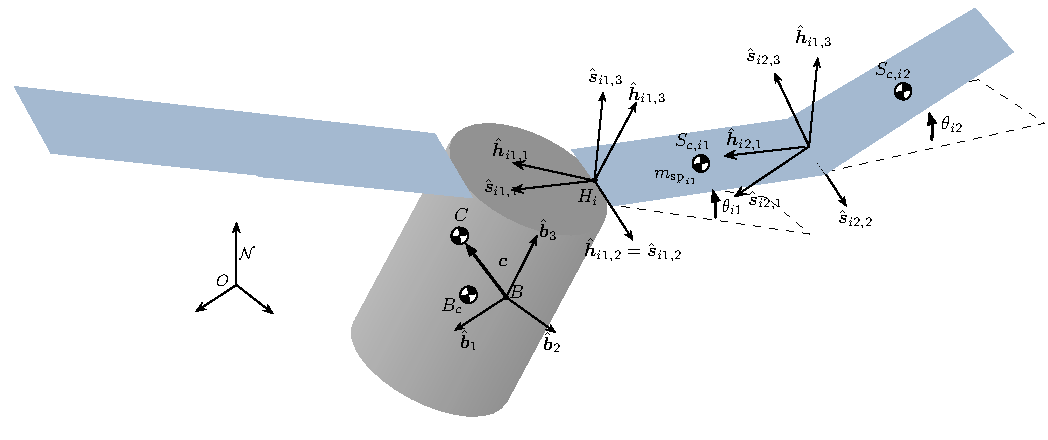
\includegraphics[]{Figures/Flex_Slosh_Figure}
	\caption{Frame and variable definitions used for formulation}
	\label{fig:Flex_Slosh_Figure}
\end{figure} 

There are six coordinate frames defined for this formulation. The inertial reference frame is indicated by \frameDefinition{N}. The body fixed coordinate frame, \frameDefinition{B}, which is anchored to the hub and can be oriented in any direction. The first solar panel frame, $\mathcal{S}_{i1}:\{\hat{\bm s}_{i1,1},\hat{\bm s}_{i1,2},\hat{\bm s}_{i1,3}\}$, is a frame with its origin located at its corresponding hinge location, $H_{i1}$. The $\mathcal{S}_{i1}$ frame is oriented such that $\hat{\bm{s}}_{i1,1}$ points antiparallel to the center of mass of the first solar panel, $S_{c,i1}$. The $\hat{\bm{s}}_{i1,2}$ axis is defined as the rotation axis that would yield a positive $\theta_{i1}$ using the right-hand rule. The distance from point $H_{i1}$ to point $S_{c,i1}$ is defined as $d_{i1}$. The total length of the first panel is $l_{i1}$ The hinge frame, $\mathcal{H}_{i1}:\{\hat{\bm h}_{i1,1}, \hat{\bm h}_{i1,2}, \hat{\bm h}_{i1,3} \}$, is a frame fixed with respect to the body frame, and is equivalent to the respective $\mathcal{S}_{i1}$ frame when the corresponding solar panel is undeflected.

The other two frames $\mathcal{S}_{i2}$ and $\mathcal{H}_{i2}$ are frames attached to the second solar panel. The $\mathcal{H}_{i2}$ frame is located at the joint between the two solar panels and $\hat{\bm h}_{i1,2} = \hat{\bm h}_{i2,2}$. The $\hat{\bm h}_{i2,1}$ completes the definition of the $\mathcal{H}_{i2}$ frame and can be oriented in any direction while orthogonal to the $\hat{\bm h}_{i2,2}$ axis. This allows for the simulation to model undeployed solar panels for example and defines the undeflected direction of the second solar panel. The $\mathcal{S}_{i2}$ by being equal to the $\mathcal{H}_{i2}$ when the second solar panel is undeflected from its equilibrium point and rotates about the $\hat{\bm h}_{i2,2}$ axis.

There are a few more key locations that need to be defined. Point $B$ is the origin of the body frame, and can have any location with respect to the hub. Point $B_c$ is the location of the center of mass of the rigid hub.

Using the variables and frames defined, the following section outlines the derivation of equations of motion for the spacecraft. 

\subsection{Derivation of Equations of Motion - Newtonian Mechanics}

\subsubsection{Rigid Spacecraft Hub Translational Motion}

Following a similar derivation as in previous work \cite{Allard2016rz}, the derivation begins with Newton's first law for the center of mass of the spacecraft.
\begin{equation}
	\ddot{\bm r}_{C/N} = \frac{\bm{F}}{m_{\text{\text{sc}}}}
	\label{eq:Newtons1Law}
\end{equation}
Ultimately the acceleration of the body frame or point $B$ is desired
\begin{equation}
	\ddot{\bm r}_{B/N} = \ddot{\bm r}_{C/N}-\ddot{\bm c}
	\label{eq:RcRbacc}
\end{equation}
The definition of $\bm{c}$ the location of the center of mass of the entire spacecraft, can be seen in Eq. (\ref{eq:c}).
\begin{equation}
	\bm{c} = \frac{1}{m_{\text{sc}}}\Big[m_{\text{\text{hub}}}\bm{r}_{B_{c}/B} +\sum_{i=1}^{N_{S}}\big(m_{\text{sp}_{i1}}\bm{r}_{S_{c,i1}/B}+m_{\text{sp}_{i2}}\bm{r}_{S_{c,i2}/B}\big)\Big]
	\label{eq:c} 
\end{equation}
To find the inertial time derivative of $\bm{c}$, it is first necessary to find the time derivative of $\bm{c}$ with respect to the body frame. A time derivative of any vector, $\bm{v}$, with respect to the body frame is denoted by $\bm{v}'$; the inertial time derivative is labeled as $\dot{\bm{v}}$. The first and second body-relative time derivatives of $\bm{c}$ can be seen in Eqs. (\ref{eq:cprime}) and (\ref{eq:cdprime}).
\begin{align}
	\bm{c}' &= \frac{1}{m_{\text{sc}}}\sum_{i=1}^{N_{S}}\big(m_{\text{sp}_{i1}}\bm{r}'_{S_{c,i1}/B}+m_{\text{sp}_{i2}}\bm{r}'_{S_{c,i2}/B}\big)
	\label{eq:cprime}
	\\
	\bm{c}'' &= \frac{1}{m_{\text{sc}}}\sum_{i=1}^{N_{S}}\big(m_{\text{sp}_{i1}}\bm{r}''_{S_{c,i1}/B}+m_{\text{sp}_{i2}}\bm{r}''_{S_{c,i2}/B}\big)
	\label{eq:cdprime}
\end{align}
The vector $\bm{r}_{S_{c,i1}/B}$ is readily defined using the $\hat{\bm{s}}_{i,1}$ axis
\begin{equation}
	\bm{r}_{S_{c,{i1}}/B} = 	\bm{r}_{H_{i1}/B} -d_{i1} \bm{\hat{s}}_{i1,1}
	\label{eq:rcgspi1}
\end{equation}
The vector $\bm{r}_{S_{c,i2}/B}$ is defined similarly
\begin{equation}
	\bm{r}_{S_{c,{i2}}/B} = 	\bm{r}_{H_{i1}/B} -l_{i1} \bm{\hat{s}}_{i1,1} - d_{i2}\bm{\hat{s}}_{i2,1}
	\label{eq:rcgspi2}
\end{equation}
Now the first and second time derivatives with respect to the body frame of $\bm{r}_{S_{c,i1}/B}$ are taken
\begin{align}
	\bm{r}'_{S_{c,i1}/B} &= d_{i1} \dot{\theta}_{i1} \bm{\hat{s}}_{i1,3}
	\label{eq:drcgspi1}
	\\
	\bm{r}''_{S_{c,i1}/B} &= d_{i1} \bm{\hat{s}}_{i1,3} \ddot{\theta}_{i1} + d_{i1} \dot{\theta}_{i1}^2 \bm{\hat{s}}_{i1,1}
	\label{eq:ddrcgspi1}
\end{align}
Similarly the body time derivatives of $\bm{r}_{S_{c,i2}/B}$ are defined in the following
\begin{align}
	\bm{r}'_{S_{c,i2}/B} &= l_{i1} \dot{\theta}_{i1} \bm{\hat{s}}_{i1,3} + d_{i2}\big(\dot{\theta}_{i1} + \dot{\theta}_{i2}\big)\bm{\hat{s}}_{i2,3}
	\label{eq:drcgspi2}
	\\
	\bm{r}''_{S_{c,i2}/B} &= (l_{i1} \bm{\hat{s}}_{i1,3} + d_{i2} \bm{\hat{s}}_{i2,3}) \ddot{\theta}_{i1} + d_{i2} \bm{\hat{s}}_{i2,3} \ddot{\theta}_{i2} + l_{i1} \dot{\theta}_{i1}^2 \bm{\hat{s}}_{i1,1} + d_{i2}\big(\dot{\theta}_{i1} + \dot{\theta}_{i2}\big)^2\bm{\hat{s}}_{i2,1}
	\label{eq:ddrcgspi2}
\end{align}
Eqs.~\eqref{eq:cprime} and ~\eqref{eq:cdprime} are next reformulated to include these new definitions:
\begin{equation}
	\bm{c}' = \frac{1}{m_{\text{sc}}}\sum_{i=1}^{N_{S}}\bigg(m_{\text{sp}_{i1}}\Big[d_{i1} \dot{\theta}_{i1} \bm{\hat{s}}_{i1,3}\Big]+m_{\text{sp}_{i2}}\Big[l_{i1} \dot{\theta}_{i1} \bm{\hat{s}}_{i1,3} + d_{i2}\big(\dot{\theta}_{i1} + \dot{\theta}_{i2}\big)\bm{\hat{s}}_{i2,3}\Big]\bigg)
	\label{eq:cprime2}
\end{equation}
\begin{multline}
	\bm{c}'' = \frac{1}{m_{\text{sc}}}\sum_{i=1}^{N_{S}}\bigg(m_{\text{sp}_{i1}}d_{i1} \big(\ddot{\theta}_{i1} \bm{\hat{s}}_{i1,3} + \dot{\theta}_{i1}^2 \bm{\hat{s}}_{i1,1}\big)\\
	+m_{\text{sp}_{i2}}\Big[l_{i1} \left(\ddot{\theta}_{i1} \bm{\hat{s}}_{i1,3} + \dot{\theta}_{i1}^2 \bm{\hat{s}}_{i1,1}\right) + d_{i2}\big(\ddot{\theta}_{i1} + \ddot{\theta}_{i2}\big)\bm{\hat{s}}_{i2,3} + d_{i2}\big(\dot{\theta}_{i1} + \dot{\theta}_{i2}\big)^2\bm{\hat{s}}_{i2,1}\Big]\bigg)
	\label{eq:cdprime2}
\end{multline}
Using the transport theorem\cite{schaub} yields the following definition for $\ddot{\bm c}$
\begin{equation}
	\ddot{\bm c} = \bm{c}'' + 2\bm\omega_{\cal B/N}\times\bm{c}'+\dot{\bm\omega}_{\cal B/N}\times\bm{c}+\bm\omega_{\cal B/N}\times\left(\bm\omega_{\cal B/N}\times\bm{c}\right)
	\label{eq:cddot}
\end{equation}
Eq.~\eqref{eq:RcRbacc} is updated to include Eq.~\eqref{eq:cddot}
\begin{equation}
	\ddot{\bm r}_{B/N} = \ddot{\bm r}_{C/N}-\bm{c}'' - 2\bm\omega_{\cal B/N}\times\bm{c}'-\dot{\bm\omega}_{\cal B/N}\times\bm{c}-\bm\omega_{\cal B/N}\times\left(\bm\omega_{\cal B/N}\times\bm{c}\right)
	\label{eq:Rbddot}
\end{equation}
Substituting Eq.\eqref{eq:cdprime2} into Eq.\eqref{eq:Rbddot} and moving the second order state variables to the left hand side results in
\begin{multline}
	\ddot{\bm r}_{B/N} + \dot{\bm\omega}_{\cal B/N}\times\bm{c} +  \frac{1}{m_{\text{sc}}}\sum_{i=1}^{N_{S}}\bigg(\Big[m_{\text{sp}_{i1}}d_{i1} \bm{\hat{s}}_{i1,3} +m_{\text{sp}_{i2}}l_{i1} \bm{\hat{s}}_{i1,3}+m_{\text{sp}_{i2}} d_{i2}\bm{\hat{s}}_{i2,3}\Big]\ddot{\theta}_{i1} +m_{\text{sp}_{i2}} d_{i2} \bm{\hat{s}}_{i2,3}\ddot{\theta}_{i2}\bigg) \\
	= \ddot{\bm r}_{C/N}-\frac{1}{m_{\text{sc}}}\sum_{i=1}^{N_{S}}\bigg(m_{\text{sp}_{i1}}d_{i1} \dot{\theta}_{i1}^2 \bm{\hat{s}}_{i1,1} +m_{\text{sp}_{i2}}\Big[l_{i1} \dot{\theta}_{i1}^2 \bm{\hat{s}}_{i1,1} + d_{i2}\big(\dot{\theta}_{i1} + \dot{\theta}_{i2}\big)^2\bm{\hat{s}}_{i2,1}\Big]\bigg) \\
	- 2\bm\omega_{\cal B/N}\times\bm{c}'-\bm\omega_{\cal B/N}\times\left(\bm\omega_{\cal B/N}\times\bm{c}\right)
	\label{eq:Rbddot2}
\end{multline}
Introducing the tilde matrix\cite{schaub} to replace the cross product operators and multiplying both sides by $m_\text{sc}$ simplifies the equation to
\begin{multline}
	m_\text{sc} \ddot{\bm r}_{B/N} -m_\text{sc} [\tilde{\bm{c}}] \dot{\bm\omega}_{\cal B/N} +  \sum_{i=1}^{N_{S}}\bigg(\Big[m_{\text{sp}_{i1}}d_{i1} \bm{\hat{s}}_{i1,3} +m_{\text{sp}_{i2}}l_{i1} \bm{\hat{s}}_{i1,3}+m_{\text{sp}_{i2}} d_{i2}\bm{\hat{s}}_{i2,3}\Big]\ddot{\theta}_{i1} +m_{\text{sp}_{i2}} d_{i2} \bm{\hat{s}}_{i2,3}\ddot{\theta}_{i2}\bigg) \\
	= \bm F - 2m_\text{sc} [\tilde{\bm\omega}_{\cal B/N}] \bm c'- m_\text{sc} [\tilde{\bm\omega}_{\cal B/N}][\tilde{\bm\omega}_{\cal B/N}]\bm{c}\\
	-\sum_{i=1}^{N_{S}}\bigg(m_{\text{sp}_{i1}}d_{i1} \dot{\theta}_{i1}^2 \bm{\hat{s}}_{i1,1} +m_{\text{sp}_{i2}}\Big[l_{i1} \dot{\theta}_{i1}^2 \bm{\hat{s}}_{i1,1} + d_{i2}\big(\dot{\theta}_{i1} + \dot{\theta}_{i2}\big)^2\bm{\hat{s}}_{i2,1}\Big]\bigg) 
	\label{eq:Rbddot3}
\end{multline}

Equation~\eqref{eq:Rbddot3} is the translational motion equation and is the first EOM needed to describe the motion of the spacecraft. The following section develops the rotational EOM.

\subsubsection{Rigid Spacecraft Hub Rotational Motion}

Starting with Euler's equation when the body fixed coordinate frame origin is not coincident with the center of mass of the body\cite{schaub}
\begin{equation}
	\bm{\dot{H}}_{\text{sc},B} = \bm{L}_B+m_{\text{\text{sc}}}\ddot{\bm r}_{B/N}\times\bm{c}
	\label{eq:Euler}
\end{equation}
where $\bm{L}_B$ is the total external torque about point $B$. The definition of the angular momentum vector of the spacecraft about point $B$ is
\begin{multline}
	\bm{H}_{\text{sc},B} = [I_{\text{hub},B_c}] \bm\omega_{\cal B/N} + m_{\text{hub}} \bm{r}_{B_c/B}\times\bm{\dot{r}}_{B_c/B} \\ +\sum\limits_{i=1}^{N_S}\Big( [I_{\text{sp}_{i1},S_{c,i1}}] \bm\omega_{\cal B/N} + \dot{\theta}_{i1} I_{s_{i1,2}}\bm{\hat{s}}_{i1,2}+m_{\text{sp}_{i1}} \bm{r}_{S_{c,i1}/B} \times \dot{\bm r}_{S_{c,i1}/B}\\
	+ [I_{\text{sp}_{i2},S_{c,i2}}] \bm\omega_{\cal B/N} + \big(\dot{\theta}_{i1} + \dot{\theta}_{i2}\big) I_{s_{i2,2}}\bm{\hat{s}}_{i2,2}+m_{\text{sp}_{i2}} \bm{r}_{S_{c,i2}/B} \times \dot{\bm r}_{S_{c,i2}/B}\Big)
	\label{eq:Hb2}
\end{multline}
Both solar panel inertia's about their center of masses' are assumed to be defined along principal inertia axes and are of the form
\begin{equation}
	[I_{\text{sp}_{i1},S_{c,i1}}] = {\vphantom{\begin{bmatrix}
				I_{s_{i1,1}} & 0 & 0 \\
				0 & I_{s_{i1,2}} & 0 \\
				0 & 0 & I_{s_{i1,3}}
	\end{bmatrix}}}^{\mathcal{S}_{i1}\!}{\begin{bmatrix}
			I_{s_{i1,1}} & 0 & 0 \\
			0 & I_{s_{i1,2}} & 0 \\
			0 & 0 & I_{s_{i1,3}}
	\end{bmatrix}} 
	\label{eq:IspMatrix}
\end{equation}

\begin{equation}
	[I_{\text{sp}_{i2},S_{c,i2}}] = {\vphantom{\begin{bmatrix}
				I_{s_{i2,1}} & 0 & 0 \\
				0 & I_{s_{i2,2}} & 0 \\
				0 & 0 & I_{s_{i2,3}}
	\end{bmatrix}}}^{\mathcal{S}_{i2}\!}{\begin{bmatrix}
			I_{s_{i2,1}} & 0 & 0 \\
			0 & I_{s_{i2,2}} & 0 \\
			0 & 0 & I_{s_{i2,3}}
	\end{bmatrix}} 
\end{equation}
Now the inertial time derivative of Eq. \eqref{eq:Hb2} is taken and yields
\begin{multline}
	\dot{\bm{H}}_{\text{sc},B} = [I_{\text{hub},B_c}] \dot{\bm\omega}_{\cal B/N} + \bm\omega_{\cal B/N} \times [I_{\text{hub},B_c}] \bm\omega_{\cal B/N} + m_{\text{hub}} \bm{r}_{B_c/B}\times\ddot{\bm r}_{B_c/B}\\ +\sum\limits_{i=1}^{N_S} \biggl( [I'_{\text{sp}_{i1},S_{c,i1}}] \bm\omega_{\cal B/N} + [I_{\text{sp}_{i1},S_{c,i1}}] \dot{\bm\omega}_{\cal B/N} + \bm\omega_{\cal B/N} \times [I_{\text{sp}_{i1},S_{c,i1}}] \bm\omega_{\cal B/N}\\ 
	+ \ddot{\theta}_{i1} I_{s_{i1,2}}\bm{\hat{s}}_{i1,2}+ \bm\omega_{\cal B/N} \times \dot{\theta}_{i1} I_{s_{i1,2}}\bm{\hat{s}}_{i1,2} +m_{\text{sp}_{i1}} \bm{r}_{S_{c,i1}/B} \times \ddot{\bm r}_{S_{c,i1}/B}\\
	+ [I'_{\text{sp}_{i2},S_{c,i2}}] \bm\omega_{\cal B/N} + [I_{\text{sp}_{i2},S_{c,i2}}] \dot{\bm\omega}_{\cal B/N} + \bm\omega_{\cal B/N} \times [I_{\text{sp}_{i2},S_{c,i2}}] \bm\omega_{\cal B/N}\\ 
	+ \big(\ddot{\theta}_{i1} + \ddot{\theta}_{i2}\big) I_{s_{i2,2}}\bm{\hat{s}}_{i2,2}+ \bm\omega_{\cal B/N} \times \big(\dot{\theta}_{i1} + \dot{\theta}_{i2}\big) I_{s_{i2,2}}\bm{\hat{s}}_{i2,2} +m_{\text{sp}_{i1}} \bm{r}_{S_{c,i2}/B} \times \ddot{\bm r}_{S_{c,i2}/B}\biggr)
	\label{eq:Hbdot}
\end{multline}
The terms $\ddot{\bm r}_{B_c/B}$, $\ddot{\bm r}_{S_{c,i1}/B}$ and $\ddot{\bm r}_{S_{c,i2}/B}$ are found using the transport theorem and knowing that $\bm{r}_{B_c/B}$ is fixed with respect to the body frame.
\begin{align}
	\ddot{\bm r}_{B_c/B} &= \bm{\dot{\omega}}_{\cal B/N} \times \bm{r}_{B_c/B} + \bm\omega_{\cal B/N} \times (\bm\omega_{\cal B/N} \times \bm{r}_{B_c/B})
	\label{eq:rbddot}
	\\
	\ddot{\bm r}_{S_{c,i1}/B} &= \bm{r}''_{S_{c,i1}/B} + 2 \bm\omega_{\cal B/N} \times \bm{r}'_{S_{c,i1}/B} +  \dot{\bm\omega}_{\cal B/N} \times \bm{r}_{S_{c,i1}/B} + \bm\omega_{\cal B/N} \times (\bm\omega_{\cal B/N} \times \bm{r}_{S_{c,i1}/B})
	\label{eq:rsddot}
	\\
	\ddot{\bm r}_{S_{c,i2}/B} &= \bm{r}''_{S_{c,i2}/B} + 2 \bm\omega_{\cal B/N} \times \bm{r}'_{S_{c,i2}/B} +  \dot{\bm\omega}_{\cal B/N} \times \bm{r}_{S_{c,i2}/B} + \bm\omega_{\cal B/N} \times (\bm\omega_{\cal B/N} \times \bm{r}_{S_{c,i2}/B})
	\label{eq:rsddot2}
\end{align}
Incorporating Eqs.~\eqref{eq:rbddot} -~\eqref{eq:rsddot2} into Eq.~\eqref{eq:Hbdot} results in

\begin{multline}
	\dot{\bm{H}}_{\text{sc},B} = [I_{\text{hub},B_c}] \dot{\bm\omega}_{\cal B/N} + \bm\omega_{\cal B/N} \times [I_{\text{hub},B_c}] \bm\omega_{\cal B/N} + m_{\text{hub}} \bm{r}_{B_c/B}\times ( \dot{\bm\omega}_{\cal B/N}\times \bm{r}_{B_c/B}) \\+ m_{\text{hub}} \bm{r}_{B_c/B}\times\Big[\bm\omega_{\cal B/N} \times (\bm\omega_{\cal B/N} \times \bm{r}_{B_c/B})\Big] +\sum\limits_{i=1}^{N_S} \biggl( [I'_{\text{sp}_{i1},S_{c,i1}}] \bm\omega_{\cal B/N} + [I_{\text{sp}_{i1},S_{c,i1}}] \dot{\bm\omega}_{\cal B/N} \\+ \bm\omega_{\cal B/N} \times [I_{\text{sp}_{i1},S_{c,i1}}] \bm\omega_{\cal B/N} 
	+ \ddot{\theta}_{i1} I_{s_{i1,2}}\bm{\hat{s}}_{i1,2}+ \bm\omega_{\cal B/N} \times \dot{\theta}_{i1} I_{s_{i1,2}}\bm{\hat{s}}_{i1,2} 
	+m_{\text{sp}_{i1}} \bm{r}_{S_{c,i1}/B} \times \bm{r}''_{S_{c,i1}/B}\\ + 2 m_{\text{sp}_{i1}} \bm{r}_{S_{c,i1}/B} \times \Big( \bm\omega_{\cal B/N} \times \bm{r}'_{S_{c,i1}/B}\Big)
	+m_{\text{sp}_{i1}} \bm{r}_{S_{c,i1}/B} \times \Big( \dot{\bm\omega}_{\cal B/N} \times \bm{r}_{S_{c,i1}/B}\Big) \\+m_{\text{sp}_{i1}} \bm{r}_{S_{c,i1}/B} \times \Big[ \bm\omega_{\cal B/N} \times (\bm\omega_{\cal B/N} \times \bm{r}_{S_{c,i1}/B})\Big]
	+ [I'_{\text{sp}_{i2},S_{c,i2}}] \bm\omega_{\cal B/N} + [I_{\text{sp}_{i2},S_{c,i2}}] \dot{\bm\omega}_{\cal B/N} \\+ \bm\omega_{\cal B/N} \times [I_{\text{sp}_{i2},S_{c,i2}}] \bm\omega_{\cal B/N} 
	+ \big(\ddot{\theta}_{i1} + \ddot{\theta}_{i2}\big) I_{s_{i2,2}}\bm{\hat{s}}_{i2,2}+ \bm\omega_{\cal B/N} \times \big(\dot{\theta}_{i1} + \dot{\theta}_{i2}\big) I_{s_{i2,2}}\bm{\hat{s}}_{i2,2} \\
	+m_{\text{sp}_{i2}} \bm{r}_{S_{c,i2}/B} \times \bm{r}''_{S_{c,i2}/B} + 2 m_{\text{sp}_{i2}} \bm{r}_{S_{c,i2}/B} \times \Big(\bm\omega_{\cal B/N} \times \bm{r}'_{S_{c,i2}/B}\Big)\\
	+m_{\text{sp}_{i2}} \bm{r}_{S_{c,i2}/B} \times \Big(\dot{\bm\omega}_{\cal B/N} \times \bm{r}_{S_{c,i2}/B}\Big) +m_{\text{sp}_{i2}} \bm{r}_{S_{c,i2}/B} \times \Big[\bm\omega_{\cal B/N} \times (\bm\omega_{\cal B/N} \times \bm{r}_{S_{c,i2}/B})\Big]\biggr)
	\label{eq:Hbdot3}
\end{multline}	

Applying the parallel axis theorem the following inertia tensor terms are defined as
\begin{align}
	[I_{\text{hub},B}] &= [I_{\text{hub},B_c}] + m_{\text{hub}}[\bm{\tilde{r}}_{B_c/B}] [\bm{\tilde{r}}_{B_c/B}]^T
	\label{eq:IHubB}
	\\
	[I_{\text{sp}_{i1},B}] &= [I_{\text{sp}_{i1},S_{c,i1}}] + m_{\text{sp}_{i1}}[\bm{\tilde{r}}_{S_{c,i1}/B}] [\bm{\tilde{r}}_{S_{c,{i1}}/B}]^T
	\\
	[I_{\text{sp}_{i2},B}] &= [I_{\text{sp}_{i2},S_{c,i2}}] + m_{\text{sp}_{i2}}[\bm{\tilde{r}}_{S_{c,i2}/B}] [\bm{\tilde{r}}_{S_{c,{i2}}/B}]^T
	\\
	[I_{\text{sc},B}] &= [I_{\text{hub},B}] + \sum\limits_{i=1}^{N_S}\Big( [I_{\text{sp}_{i1},B}] + [I_{\text{sp}_{i2},B}]\Big)
	\label{eq:IscB}
\end{align}
Because the tilde matrices are skew-symmetric, taking the body-relative time derivative of Equation~\eqref{eq:IscB} yields
\begin{multline}
	[I'_{\text{sc},B}] = \sum\limits_{i=1}^{N_S} \Big[[I'_{\text{sp}_{i1},S_{c,i1}}] - m_{\text{sp}_{i1}}\left([\bm{\tilde{r}}'_{S_{c,{i1}}/B}] [\bm{\tilde{r}}_{S_{c,{i1}}/B}] + [\bm{\tilde{r}}_{S_{c,{i1}}/B}] [\bm{\tilde{r}}'_{S_{c,{i1}}/B}]\right)\\
	+[I'_{\text{sp}_{i2},S_{c,i2}}] - m_{\text{sp}_{i2}}\left([\bm{\tilde{r}}'_{S_{c,{i2}}/B}] [\bm{\tilde{r}}_{S_{c,{i2}}/B}] + [\bm{\tilde{r}}_{S_{c,{i2}}/B}] [\bm{\tilde{r}}'_{S_{c,{i2}}/B}]\right)\Big]
	\label{eq:IprimeScB}
\end{multline}
$[I'_{\text{sp}_{i1},S_{c,i1}}]$ needs to be defined and can be conveniently expressed by leveraging the assumption that the inertia matrix is diagonal (as seen in Eq. \eqref{eq:IspMatrix}) and is written in terms of its base vectors:
\begin{equation}
	[I_{\text{sp}_{i1},S_{c,i1}}] = I_{s_{i1,1}}\hat{\bm s}_{i1,1}\hat{\bm s}_{i1,1}^{T}+I_{s_{i1,2}}\hat{\bm s}_{i1,2}\hat{\bm s}_{i1,2}^{T}+I_{s_{i1,3}}\hat{\bm s}_{i1,3}\hat{\bm s}_{i1,3}^{T}
	\label{eq:iprime}
\end{equation}
Taking the body time derivative of Eq.~\eqref{eq:iprime} results in
\begin{multline}
	[I'_{\text{sp}_{i1},S_{c,i1}}] = I_{s_{i1,1}}\hat{\bm s}'_{i1,1}\hat{\bm s}_{i1,1}^{T}+I_{s_{i1,1}}\hat{\bm s}_{i1,1}\hat{\bm s}_{i1,1}'^{T}+I_{s_{i1,2}}\hat{\bm s}'_{i1,2}\hat{\bm s}_{i1,2}^{T}\\
	+I_{s_{i1,2}}\hat{\bm s}_{i1,2}\hat{\bm s}_{i1,2}'^{T}+I_{s_{i1,3}}\hat{\bm s}'_{i1,3}\hat{\bm s}_{i1,3}^{T}+I_{s_{i1,3}}\hat{\bm s}_{i1,3}\hat{\bm s}_{i1,3}'^{T}
	\label{eq:iprime2}
\end{multline}
Using the transport theorem for each basis vector, j, in the $\bm{\hat{s}}_{i1}$ frame: $\hat{\bm s}'_{i1,j} = \bm\omega_{\cal{S}_{\textit{i1}}/\cal{B}}\times\hat{\bm s}_{i1,j}=\dot{\theta}_{i1}\hat{\bm s}_{i1,2}\times\hat{\bm s}_{i1,j}$, applying this to Eq.~\eqref{eq:iprime2}, evaluating the cross products, and simplifying results in
\begin{equation}
	[I'_{\text{sp}_{i1},S_{c,i1}}] = \dot{\theta}_{i1}(I_{s_{i1,3}}-I_{s_{i1,1}})(\hat{\bm s}_{i1,1}\hat{\bm s}_{i1,3}^{T}+\hat{\bm s}_{i1,3}\hat{\bm s}_{i1,1}^{T})
	\label{eq:iprime3}
\end{equation}

Applying the same methodology for $[I'_{\text{sp}_{i2},S_{c,i2}}]$ and using the following definition: $\hat{\bm s}'_{i2,j} = \bm\omega_{\cal{S}_{\textit{i2}}/\cal{B}}\times\hat{\bm s}_{i2,j}=\big(\dot{\theta}_{i1} + \dot{\theta}_{i2} \big)\hat{\bm s}_{i2,2}\times\hat{\bm s}_{i2,j}$ results in 
\begin{equation}
	[I'_{\text{sp}_{i2},S_{c,i2}}] = \big(\dot{\theta}_{i1}+\dot{\theta}_{i2}\big)(I_{s_{i2,3}}-I_{s_{i2,1}})(\hat{\bm s}_{i2,1}\hat{\bm s}_{i2,3}^{T}+\hat{\bm s}_{i2,3}\hat{\bm s}_{i2,1}^{T})
	\label{eq:iprime4}
\end{equation}
Substituting Eq.~\eqref{eq:iprime3} and Eq.~\eqref{eq:iprime4} into Eq.~\eqref{eq:Hbdot3} and using Eq.~\eqref{eq:IscB} to simplify results in Eq.~\eqref{eq:Hbdot4}. The Jacobi Identity, $(\bm a \times \bm b)\times \bm c = \bm a \times (\bm b\times \bm c) - \bm b \times (\bm a\times \bm c)$, is used to combine terms.\\
Factoring out $\dot{\bm\omega}_{\cal B/N}$ and, selectively, $\bm{\omega}_{\cal B/N}$ and utilizing the tilde matrix transforms Eq. \ref{eq:Hbdot3} into Eq. \ref{eq:Hbdot17} so that $[I_{\text{sc},B}]$ can be extracted.
\begin{multline}
	\dot{\bm{H}}_{\text{sc},B} = \bigg([I_{\text{hub},B_c}]  - m_{\text{hub}} [\tilde{\bm{r}}_{B_c/B}] [\tilde{\bm{r}}_{B_c/B}] + 
	\sum\limits_{i=1}^{N_S} \Big([I_{\text{sp}_{i1},S_{c,i1}}]+ [I_{\text{sp}_{i2},S_{c,i2}}] - m_{\text{sp}_{i1}} [\tilde{\bm{r}}_{S_{c,i1}/B}] [\tilde{\bm{r}}_{S_{c,i1}/B}] \\
	- m_{\text{sp}_{i2}} [\tilde{\bm{r}}_{S_{c,i2}/B}] [\tilde{\bm{r}}_{S_{c,i2}/B}]   \Big)\bigg)\dot{\bm\omega}_{\cal B/N}	+ \bm\omega_{\cal B/N} \times \bigg([I_{\text{hub},B_c}] - m_{\text{hub}} [\tilde{\bm{r}}_{B_c/B}] [\tilde{\bm{r}}_{B_c/B}] + \\
	\sum\limits_{i=1}^{N_S}\Big(  [I_{\text{sp}_{i1},S_{c,i1}}]+ [I_{\text{sp}_{i2},S_{c,i2}}] - m_{\text{sp}_{i1}} [\tilde{\bm{r}}_{S_{c,i1}/B}] [\tilde{\bm{r}}_{S_{c,i1}/B}] - m_{\text{sp}_{i2}} [\tilde{\bm{r}}_{S_{c,i2}/B}] [\tilde{\bm{r}}_{S_{c,i2}/B}]  \Big) \bigg) \bm\omega_{\cal B/N} \\ 
	+\sum\limits_{i=1}^{N_S} \biggl( [I'_{\text{sp}_{i1},S_{c,i1}}] \bm\omega_{\cal B/N} 
	+ \ddot{\theta}_{i1} I_{s_{i1,2}}\bm{\hat{s}}_{i1,2}+ \bm\omega_{\cal B/N} \times \dot{\theta}_{i1} I_{s_{i1,2}}\bm{\hat{s}}_{i1,2}	+m_{\text{sp}_{i1}} \bm{r}_{S_{c,i1}/B} \times \bm{r}''_{S_{c,i1}/B} \\
	+ 2 m_{\text{sp}_{i1}} \bm{r}_{S_{c,i1}/B} \times \Big( \bm\omega_{\cal B/N} \times \bm{r}'_{S_{c,i1}/B}\Big)	+ [I'_{\text{sp}_{i2},S_{c,i2}}] \bm\omega_{\cal B/N} 
	+ \big(\ddot{\theta}_{i1} + \ddot{\theta}_{i2}\big) I_{s_{i2,2}}\bm{\hat{s}}_{i2,2}+ \\
	\bm\omega_{\cal B/N} \times \big(\dot{\theta}_{i1} + \dot{\theta}_{i2}\big) I_{s_{i2,2}}\bm{\hat{s}}_{i2,2}
	+m_{\text{sp}_{i2}} \bm{r}_{S_{c,i2}/B} \times \bm{r}''_{S_{c,i2}/B} + 2 m_{\text{sp}_{i2}} \bm{r}_{S_{c,i2}/B} \times \Big(\bm\omega_{\cal B/N} \times \bm{r}'_{S_{c,i2}/B}\Big)\biggr)
	\label{eq:Hbdot17}
\end{multline}
$[I_{\text{sc},B}]$ is substituted in from Eq. \ref{eq:IHubB} through Eq. \ref{eq:IscB}:
\begin{multline}
	\dot{\bm{H}}_{\text{sc},B} = [I_{\text{sc},B}]\dot{\bm\omega}_{\cal B/N}	+ \bm\omega_{\cal B/N} \times [I_{\text{sc},B}] \bm\omega_{\cal B/N} \\ 
	+\sum\limits_{i=1}^{N_S} \biggl( [I'_{\text{sp}_{i1},S_{c,i1}}] \bm\omega_{\cal B/N} 
	+ \ddot{\theta}_{i1} I_{s_{i1,2}}\bm{\hat{s}}_{i1,2}+ \bm\omega_{\cal B/N} \times \dot{\theta}_{i1} I_{s_{i1,2}}\bm{\hat{s}}_{i1,2}	+m_{\text{sp}_{i1}} \bm{r}_{S_{c,i1}/B} \times \bm{r}''_{S_{c,i1}/B} \\
	+ 2 m_{\text{sp}_{i1}} \bm{r}_{S_{c,i1}/B} \times \Big( \bm\omega_{\cal B/N} \times \bm{r}'_{S_{c,i1}/B}\Big)	+ [I'_{\text{sp}_{i2},S_{c,i2}}] \bm\omega_{\cal B/N} 
	+ \big(\ddot{\theta}_{i1} + \ddot{\theta}_{i2}\big) I_{s_{i2,2}}\bm{\hat{s}}_{i2,2}+ \\
	\bm\omega_{\cal B/N} \times \big(\dot{\theta}_{i1} + \dot{\theta}_{i2}\big) I_{s_{i2,2}}\bm{\hat{s}}_{i2,2}
	+m_{\text{sp}_{i2}} \bm{r}_{S_{c,i2}/B} \times \bm{r}''_{S_{c,i2}/B} + 2 m_{\text{sp}_{i2}} \bm{r}_{S_{c,i2}/B} \times \Big(\bm\omega_{\cal B/N} \times \bm{r}'_{S_{c,i2}/B}\Big)\biggr)
	\label{eq:Hbdot18}
\end{multline}
Splitting the doubled terms:
\begin{multline}
	\dot{\bm{H}}_{\text{sc},B} = [I_{\text{sc},B}]\dot{\bm\omega}_{\cal B/N}	+ \bm\omega_{\cal B/N} \times [I_{\text{sc},B}] \bm\omega_{\cal B/N} \\ 
	+\sum\limits_{i=1}^{N_S} \biggl( [I'_{\text{sp}_{i1},S_{c,i1}}] \bm\omega_{\cal B/N} + m_{\text{sp}_{i1}} \bm{r}_{S_{c,i1}/B} \times \Big( \bm\omega_{\cal B/N} \times \bm{r}'_{S_{c,i1}/B}\Big)
	+ \ddot{\theta}_{i1} I_{s_{i1,2}}\bm{\hat{s}}_{i1,2}+ \bm\omega_{\cal B/N} \times \dot{\theta}_{i1} I_{s_{i1,2}}\bm{\hat{s}}_{i1,2}	\\
	+m_{\text{sp}_{i1}} \bm{r}_{S_{c,i1}/B} \times \bm{r}''_{S_{c,i1}/B}
	+ m_{\text{sp}_{i1}} \bm{r}_{S_{c,i1}/B} \times \Big( \bm\omega_{\cal B/N} \times \bm{r}'_{S_{c,i1}/B}\Big)	+ [I'_{\text{sp}_{i2},S_{c,i2}}] \bm\omega_{\cal B/N} \\
	+ m_{\text{sp}_{i2}} \bm{r}_{S_{c,i2}/B} \times \Big(\bm\omega_{\cal B/N} \times \bm{r}'_{S_{c,i2}/B}\Big)
	+ \big(\ddot{\theta}_{i1} + \ddot{\theta}_{i2}\big) I_{s_{i2,2}}\bm{\hat{s}}_{i2,2} + 
	\bm\omega_{\cal B/N} \times \big(\dot{\theta}_{i1} + \dot{\theta}_{i2}\big) I_{s_{i2,2}}\bm{\hat{s}}_{i2,2}\\
	+m_{\text{sp}_{i2}} \bm{r}_{S_{c,i2}/B} \times \bm{r}''_{S_{c,i2}/B} + m_{\text{sp}_{i2}} \bm{r}_{S_{c,i2}/B} \times \Big(\bm\omega_{\cal B/N} \times \bm{r}'_{S_{c,i2}/B}\Big)\biggr)
	\label{eq:Hbdot19}
\end{multline}
Using the Jacobi Identity again, followed by tilde matrix substitution:
\begin{multline}
	\dot{\bm{H}}_{\text{sc},B} = [I_{\text{sc},B}]\dot{\bm\omega}_{\cal B/N}	+ \bm\omega_{\cal B/N} \times [I_{\text{sc},B}] \bm\omega_{\cal B/N} \\ 
	+\sum\limits_{i=1}^{N_S} \biggl( [I'_{\text{sp}_{i1},S_{c,i1}}] \bm\omega_{\cal B/N}  - m_{\text{sp}_{i1}}\Big([\tilde{\bm{r}}_{S_{c,i1}/B}][\tilde{\bm{r'}}_{S_{c,i1}/B}] + [\tilde{\bm{r'}}_{S_{c,i1}/B}][\tilde{\bm{r}}_{S_{c,i1}/B}]   \Big)\bm\omega_{\cal B/N}	
	+ \ddot{\theta}_{i1} I_{s_{i1,2}}\bm{\hat{s}}_{i1,2}\\
	+ \bm\omega_{\cal B/N} \times \dot{\theta}_{i1} I_{s_{i1,2}}\bm{\hat{s}}_{i1,2}	+m_{\text{sp}_{i1}} \bm{r}_{S_{c,i1}/B} \times \bm{r}''_{S_{c,i1}/B} 
	+ m_{\text{sp}_{i1}} \bm{r}_{S_{c,i1}/B} \times \Big( \bm\omega_{\cal B/N} \times \bm{r}'_{S_{c,i1}/B}\Big)	\\
	+ [I'_{\text{sp}_{i2},S_{c,i2}}] \bm\omega_{\cal B/N}  - m_{\text{sp}_{i2}}\Big([\tilde{\bm{r}}_{S_{c,i2}/B}] [\tilde{\bm{r'}}_{S_{c,i2}/B}] + [\tilde{\bm{r'}}_{S_{c,i2}/B}] [\tilde{\bm{r}}_{S_{c,i2}/B}]                 \Big)  \bm\omega_{\cal B/N}      
	+ \big(\ddot{\theta}_{i1} + \ddot{\theta}_{i2}\big) I_{s_{i2,2}}\bm{\hat{s}}_{i2,2} \\
	+ \bm\omega_{\cal B/N} \times \big(\dot{\theta}_{i1} + \dot{\theta}_{i2}\big) I_{s_{i2,2}}\bm{\hat{s}}_{i2,2}
	+m_{\text{sp}_{i2}} \bm{r}_{S_{c,i2}/B} \times \bm{r}''_{S_{c,i2}/B} + m_{\text{sp}_{i2}} \bm{r}_{S_{c,i2}/B} \times \Big(\bm\omega_{\cal B/N} \times \bm{r}'_{S_{c,i2}/B}\Big)\biggr)
	\label{eq:Hbdot20}
\end{multline}
Factoring out $\bm\omega_{\cal B/N}$, and substituting in from Eq. \ref{eq:IprimeScB} leaves:	
\begin{multline}
	\dot{\bm{H}}_{\text{sc},B} = [I_{\text{sc},B}] \dot{\bm\omega}_{\cal B/N} + \bm\omega_{\cal B/N} \times [I_{\text{sc},B}] \bm\omega_{\cal B/N} + [I'_{\text{sc},B}] \bm\omega_{\cal B/N}
	+  \sum\limits_{i=1}^{N_S} \bigg[ \ddot{\theta}_{i1} I_{s_{i1,2}}\bm{\hat{s}}_{i1,2}\\
	+ \bm\omega_{\cal B/N} \times \dot{\theta}_{i1} I_{s_{i1,2}}\bm{\hat{s}}_{i1,2} 
	+m_{\text{sp}_{i1}} \bm{r}_{S_{c,i1}/B} \times \bm{r}''_{S_{c,i1}/B}
	+m_{\text{sp}_{i1}} \bm\omega_{\cal B/N} \times \left(\bm{r}_{S_{c,i1}/B} \times \bm{r}'_{S_{c,i1}/B}\right)\\
	+\big(\ddot{\theta}_{i1}+\ddot{\theta}_{i2}\big) I_{s_{i2,2}}\bm{\hat{s}}_{i2,2}
	+ \bm\omega_{\cal B/N} \times \big(\dot{\theta}_{i1}+\dot{\theta}_{i2}\big) I_{s_{i2,2}}\bm{\hat{s}}_{i2,2} \\
	+m_{\text{sp}_{i2}} \bm{r}_{S_{c,i2}/B} \times \bm{r}''_{S_{c,i2}/B}
	+m_{\text{sp}_{i2}} \bm\omega_{\cal B/N} \times \left(\bm{r}_{S_{c,i2}/B} \times \bm{r}'_{S_{c,i2}/B}\right)\bigg]
	\label{eq:Hbdot4}
\end{multline}
Eqs. (\ref{eq:Euler}) and (\ref{eq:Hbdot4}) are equated and yield
\begin{multline}
	\bm{L}_B+m_{\text{sc}}\ddot{\bm r}_{B/N}\times\bm{c} = [I_{\text{sc},B}] \dot{\bm\omega}_{\cal B/N} + \bm\omega_{\cal B/N} \times [I_{\text{sc},B}] \bm\omega_{\cal B/N} + [I'_{\text{sc},B}] \bm\omega_{\cal B/N} 
	+  \sum\limits_{i=1}^{N_S} \bigg[ \ddot{\theta}_{i1} I_{s_{i1,2}}\bm{\hat{s}}_{i1,2}\\
	+ \bm\omega_{\cal B/N} \times \dot{\theta}_{i1} I_{s_{i1,2}}\bm{\hat{s}}_{i1,2} 
	+m_{\text{sp}_{i1}} \bm{r}_{S_{c,i1}/B} \times \bm{r}''_{S_{c,i1}/B}
	+m_{\text{sp}_{i1}} \bm\omega_{\cal B/N} \times \left(\bm{r}_{S_{c,i1}/B} \times \bm{r}'_{S_{c,i1}/B}\right)\\
	+\big(\ddot{\theta}_{i1}+\ddot{\theta}_{i2}\big) I_{s_{i2,2}}\bm{\hat{s}}_{i2,2}
	+ \bm\omega_{\cal B/N} \times \big(\dot{\theta}_{i1}+\dot{\theta}_{i2}\big) I_{s_{i2,2}}\bm{\hat{s}}_{i2,2} \\
	+m_{\text{sp}_{i2}} \bm{r}_{S_{c,i2}/B} \times \bm{r}''_{S_{c,i2}/B}
	+m_{\text{sp}_{i2}} \bm\omega_{\cal B/N} \times \left(\bm{r}_{S_{c,i2}/B} \times \bm{r}'_{S_{c,i2}/B}\right)\bigg]
	\label{eq:Hbdot5}
\end{multline}
Finally, using tilde matrix and simplifying yields the modified Euler equation, which is the second EOM necessary to describe the motion of the spacecraft.
\begin{multline}
	[I_{\text{sc},B}] \dot{\bm\omega}_{\cal B/N} = -[\bm{\tilde{\omega}}_{\cal B/N}] [I_{\text{sc},B}] \bm\omega_{\cal B/N} - [I'_{\text{sc},B}] \bm\omega_{\cal B/N} -  \sum\limits_{i=1}^{N_S} \bigg[ \ddot{\theta}_{i1} I_{s_{i1,2}}\bm{\hat{s}}_{i1,2}\\
	+ [\bm{\tilde{\omega}}_{\cal B/N}] \dot{\theta}_{i1} I_{s_{i1,2}}\bm{\hat{s}}_{i1,2} 
	+m_{\text{sp}_{i1}} [\tilde{\bm{r}}_{S_{c,i1}/B}] \bm{r}''_{S_{c,i1}/B}
	+m_{\text{sp}_{i1}} [\bm{\tilde{\omega}}_{\cal B/N}] [\tilde{\bm{r}}_{S_{c,i1}/B}] \bm{r}'_{S_{c,i1}/B}\\
	+\big(\ddot{\theta}_{i1}+\ddot{\theta}_{i2}\big) I_{s_{i2,2}}\bm{\hat{s}}_{i2,2}
	+ [\bm{\tilde{\omega}}_{\cal B/N}] \big(\dot{\theta}_{i1}+\dot{\theta}_{i2}\big) I_{s_{i2,2}}\bm{\hat{s}}_{i2,2} \\
	+m_{\text{sp}_{i2}} [\tilde{\bm{r}}_{S_{c,i2}/B}] \bm{r}''_{S_{c,i2}/B}
	+m_{\text{sp}_{i2}} [\bm{\tilde{\omega}}_{\cal B/N}] [\tilde{\bm{r}}_{S_{c,i2}/B}] \bm{r}'_{S_{c,i2}/B}\bigg]
	+ \bm{L}_B - m_{\text{sc}} [\tilde{\bm{c}}] \ddot{\bm r}_{B/N}
	\label{eq:Final5}
\end{multline}
However, it is desirable to place the second order state variables on the left hand side of the equation. Performing some rearranging of Eq.~\eqref{eq:Final5} results in an intermediate step. 
\begin{multline}
	m_{\text{sc}} [\tilde{\bm{c}}] \ddot{\bm r}_{B/N} + [I_{\text{sc},B}] \dot{\bm\omega}_{\cal B/N} + \sum\limits_{i=1}^{N_S} \bigg[ \ddot{\theta}_{i1} I_{s_{i1,2}}\bm{\hat{s}}_{i1,2} 
	+m_{\text{sp}_{i1}} [\tilde{\bm{r}}_{S_{c,i1}/B}] \bm{r}''_{S_{c,i1}/B}\\
	+\big(\ddot{\theta}_{i1}+\ddot{\theta}_{i2}\big) I_{s_{i2,2}}\bm{\hat{s}}_{i2,2} 
	+m_{\text{sp}_{i2}} [\tilde{\bm{r}}_{S_{c,i2}/B}] \bm{r}''_{S_{c,i2}/B}\bigg] = -[\bm{\tilde{\omega}}_{\cal B/N}] [I_{\text{sc},B}] \bm\omega_{\cal B/N} - [I'_{\text{sc},B}] \bm\omega_{\cal B/N} \\
	-  \sum\limits_{i=1}^{N_S} \bigg[
	[\bm{\tilde{\omega}}_{\cal B/N}] \dot{\theta}_{i1} I_{s_{i1,2}}\bm{\hat{s}}_{i1,2} 
	+m_{\text{sp}_{i1}} [\bm{\tilde{\omega}}_{\cal B/N}] [\tilde{\bm{r}}_{S_{c,i1}/B}] \bm{r}'_{S_{c,i1}/B}\\
	+ [\bm{\tilde{\omega}}_{\cal B/N}] \big(\dot{\theta}_{i1}+\dot{\theta}_{i2}\big) I_{s_{i2,2}}\bm{\hat{s}}_{i2,2}
	+m_{\text{sp}_{i2}} [\bm{\tilde{\omega}}_{\cal B/N}] [\tilde{\bm{r}}_{S_{c,i2}/B}] \bm{r}'_{S_{c,i2}/B}\bigg]
	+ \bm{L}_B 
	\label{eq:Finalint}
\end{multline}
Then, the second order terms are factored out:
\begin{multline}
	m_{\text{sc}} [\tilde{\bm{c}}] \ddot{\bm r}_{B/N} + [I_{\text{sc},B}] \dot{\bm\omega}_{\cal B/N} + \sum\limits_{i=1}^{N_S} \bigg[\Big(
	I_{s_{i1,2}}\bm{\hat{s}}_{i1,2} 
	+m_{\text{sp}_{i1}} d_{i1} [\tilde{\bm{r}}_{S_{c,i1}/B}] \bm{\hat{s}}_{i1,3} + I_{s_{i2,2}}\bm{\hat{s}}_{i2,2} \\
	+m_{\text{sp}_{i2}} l_{i1} [\tilde{\bm{r}}_{S_{c,i2}/B}] \bm{\hat{s}}_{i1,3}
	+m_{\text{sp}_{i2}} d_{i2} [\tilde{\bm{r}}_{S_{c,i2}/B}] \bm{\hat{s}}_{i2,3}\Big) \ddot{\theta}_{i1}
	+\Big(I_{s_{i2,2}}\bm{\hat{s}}_{i2,2} 
	+m_{\text{sp}_{i2}} [\tilde{\bm{r}}_{S_{c,i2}/B}] d_{i2}\bm{\hat{s}}_{i2,3}\Big) \ddot{\theta}_{i2} \bigg]\\
	= -[\bm{\tilde{\omega}}_{\cal B/N}] [I_{\text{sc},B}] \bm\omega_{\cal B/N} - [I'_{\text{sc},B}] \bm\omega_{\cal B/N} 
	-  \sum\limits_{i=1}^{N_S} \bigg[
	[\bm{\tilde{\omega}}_{\cal B/N}] \dot{\theta}_{i1} I_{s_{i1,2}}\bm{\hat{s}}_{i1,2} 
	+m_{\text{sp}_{i1}} d_{i1} \dot{\theta}_{i1}^2 [\tilde{\bm{r}}_{S_{c,i1}/B}] \bm{\hat{s}}_{i1,1}
	\\+m_{\text{sp}_{i2}} l_{i1} \dot{\theta}_{i1}^2 [\tilde{\bm{r}}_{S_{c,i2}/B}] \bm{\hat{s}}_{i1,1}
	+m_{\text{sp}_{i1}} [\bm{\tilde{\omega}}_{\cal B/N}] [\tilde{\bm{r}}_{S_{c,i1}/B}] \bm{r}'_{S_{c,i1}/B}
	+ [\bm{\tilde{\omega}}_{\cal B/N}] \big(\dot{\theta}_{i1}+\dot{\theta}_{i2}\big) I_{s_{i2,2}}\bm{\hat{s}}_{i2,2}
	\\
	+m_{\text{sp}_{i2}} d_{i2}\big(\dot{\theta}_{i1} + \dot{\theta}_{i2}\big)^2 [\tilde{\bm{r}}_{S_{c,i2}/B}] \bm{\hat{s}}_{i2,1}
	+m_{\text{sp}_{i2}} [\bm{\tilde{\omega}}_{\cal B/N}] [\tilde{\bm{r}}_{S_{c,i2}/B}] \bm{r}'_{S_{c,i2}/B}\bigg]
	+ \bm{L}_B
	\label{eq:Finalint}
\end{multline}

The terms $\bm{r}''_{S_{c,i1}/B}$ and $\bm{r}''_{S_{c,i2}/B}$ contain second order state variables, therefore replacing their definition seen in Eqs.~\eqref{eq:ddrcgspi1} and ~\eqref{eq:ddrcgspi2} and simplifying the expression yields
\begin{multline}
	m_{\text{sc}} [\tilde{\bm{c}}] \ddot{\bm r}_{B/N} + [I_{\text{sc},B}] \dot{\bm\omega}_{\cal B/N} + \sum\limits_{i=1}^{N_S} \bigg[  \big(I_{s_{i1,2}}\bm{\hat{s}}_{i1,2}+m_{\text{sp}_{i1}}d_{i1} [\tilde{\bm{r}}_{S_{c,i1}/B}]   \bm{\hat{s}}_{i1,3} + I_{s_{i2,2}}\bm{\hat{s}}_{i2,2}
	+m_{\text{sp}_{i2}}l_{i1} [\tilde{\bm{r}}_{S_{c,i2}/B}]  \bm{\hat{s}}_{i1,3}\\
	+m_{\text{sp}_{i2}}d_{i2} [\tilde{\bm{r}}_{S_{c,i2}/B}] \bm{\hat{s}}_{i2,3}\big) \ddot{\theta}_{i1}
	+\big( I_{s_{i2,2}}\bm{\hat{s}}_{i2,2}+m_{\text{sp}_{i2}} d_{i2} [\tilde{\bm{r}}_{S_{c,i2}/B}] \bm{\hat{s}}_{i2,3}\big)\ddot{\theta}_{i2}\bigg] 
	\\
	= -[\bm{\tilde{\omega}}_{\cal B/N}] [I_{\text{sc},B}] \bm\omega_{\cal B/N} - [I'_{\text{sc},B}] \bm\omega_{\cal B/N} 
	-  \sum\limits_{i=1}^{N_S} \bigg[
	\dot{\theta}_{i1} I_{s_{i1,2}} [\bm{\tilde{\omega}}_{\cal B/N}] \bm{\hat{s}}_{i1,2} 
	+m_{\text{sp}_{i1}} [\bm{\tilde{\omega}}_{\cal B/N}] [\tilde{\bm{r}}_{S_{c,i1}/B}] \bm{r}'_{S_{c,i1}/B} \\
	+m_{\text{sp}_{i1}}d_{i1}\dot{\theta}_{i1}^2  [\tilde{\bm{r}}_{S_{c,i1}/B}] \bm{\hat{s}}_{i1,1}
	+ \big(\dot{\theta}_{i1}+\dot{\theta}_{i2}\big) I_{s_{i2,2}}[\bm{\tilde{\omega}}_{\cal B/N}]\bm{\hat{s}}_{i2,2}
	+m_{\text{sp}_{i2}} [\bm{\tilde{\omega}}_{\cal B/N}] [\tilde{\bm{r}}_{S_{c,i2}/B}] \bm{r}'_{S_{c,i2}/B} \\
	+m_{\text{sp}_{i2}} [\tilde{\bm{r}}_{S_{c,i2}/B}] \big(l_{i1} \dot{\theta}_{i1}^2 \bm{\hat{s}}_{i1,1} + d_{i2}\big(\dot{\theta}_{i1} + \dot{\theta}_{i2}\big)^2\bm{\hat{s}}_{i2,1}\big)\bigg]
	+ \bm{L}_B 
	\label{eq:Final6}
\end{multline}


\subsubsection{Dual Linked Solar Panel Motion}

The following section follows the same derivation seen in previous work\cite{Allard2016rz} and is summarized here for convenience. 
Let $\bm L_{H_{i1}} = L_{i1,1} \hat{\bm s}_{i1,1} + L_{i1,2} \hat{\bm s}_{i1,2} + L_{i1,3} \hat{\bm s}_{i1,3}$ be the total torque acting on the first solar panel at point $H_{i1}$. The corresponding hinge torque is given through
\begin{equation}
	L_{i1,2} = - k_{i1} \theta_{i1} - c_{i1}\dot{\theta}_{i1} +  k_{i2} \theta_{i2} + c_{i2} \dot\theta_{i2} + \hat{\bm s}_{i1,2} \cdot \bm \tau_{\text{ext}_{i1},H_{i1}} + \hat{\bm s}_{i1,2} \cdot \bm{r}_{H_{i2}/H_{i1}} \times \bm F_{1/2i}
	\label{eq:hingeTorque1}
\end{equation}
Where $\bm F_{1/2i}$ is the reaction of solar panel 2 acting on solar panel 1. It is important to point out that $\bm F_{1/2i} = - \bm F_{2/1i}$. 

To define the $\bm F_{1/2i}$, $\bm F_{2/1i}$ needs to be defined. This is done performing the super particle theorem on the second solar panel:
\begin{equation}
	\bm F_{2/1i} + \bm F_{\text{ext}_{i2}} = m_{sp_{i2}} \ddot{\bm{r}}_{S_{c,i2}/N}
\end{equation}
The sum of the external forces on solar panel 2, $\bm F_{\text{ext}_{i2}}$, is separate because it does not contribute to the reaction force at the joint. With this definition $\bm F_{1/2i}$ is defined as
\begin{equation}
	\bm F_{1/2i} = \bm F_{\text{ext}_{i2}}  - m_{sp_{i2}} \ddot{\bm{r}}_{S_{c,i2}/N} 
\end{equation}
Plugging this definition into Eq.~\eqref{eq:hingeTorque1} yields
\begin{equation}
	L_{i1,2} = - k_{i1} \theta_{i1} - c_{i1}\dot{\theta}_{i1} +  k_{i2} \theta_{i2} + c_{i2} \dot\theta_{i2} + \hat{\bm s}_{i1,2} \cdot \bm \tau_{\text{ext}_{i1},H_{i1}} + \hat{\bm s}_{i1,2} \cdot \Big[\bm{r}_{H_{i2}/H_{i1}} \times \big(\bm F_{\text{ext}_{i2}}  - m_{sp_{i2}} \ddot{\bm{r}}_{S_{c,i2}/N}\big)\Big]
	\label{eq:hingeTorque2}
\end{equation}
The hinge structure produces the other two torques $L_{i1,1}$ and $L_{i1,3}$. $\bm \tau_{\text{ext}_{i1},H_{i1}}$ is the external torque on the solar panel and is projected onto the $\hat{\bm s}_{i,2}$ direction to find its contribution to $L_{i1,2}$. Gravity, for example would apply the following torque on the solar panel about point $H_{i1}$
\begin{equation}
	\bm \tau_{g,H_{i1}} = \bm r_{S_{c,i1}/H_{i1}} \times \bm F_g
\end{equation}

The inertial angular velocity vector for the solar panel frame is
\begin{equation}
	\bm\omega_{\mathcal{S}_{i1}/\mathcal{N}} = \bm\omega_{\mathcal{S}_{i1}/\mathcal{H}_{i1}} + \bm\omega_{\mathcal{H}_{i1}/\mathcal{B}} + \bm\omega_{\cal B/N}
\end{equation}
where $\bm\omega_{\mathcal{S}_{i1}/\mathcal{H}_{i1}} = \dot\theta_{i1} \hat{\bm s}_{i1,2}$.  
Because the hinge frame $\mathcal{H}_{i1}$ is fixed relative to the body frame $\mathcal{B}$ the relative angular velocity vector is $\bm\omega_{\mathcal{H}_{i1}/\mathcal{B}} = \bm 0$.  The body angular velocity vector is written in $\mathcal{S}_{i1}$-frame components as
\begin{align}
	\bm\omega_{\cal B/N} &= ( \hat{\bm s}_{i1,1} \cdot \bm\omega_{\cal B/N}) \hat{\bm s}_{i1,1}
	+ (\hat{\bm s}_{i1,2} \cdot\bm\omega_{\cal B/N}) \hat{\bm s}_{i1,2}
	+ (\hat{\bm s}_{i1,3} \cdot\bm\omega_{\cal B/N}) \hat{\bm s}_{i1,3}
	\\
	&= \omega_{s_{i1,1}} \hat{\bm s}_{i1,1} + \omega_{s_{i1,2}} \hat{\bm s}_{i1,2} + \omega_{s_{i1,3}}\hat{\bm s}_{i1,3}
\end{align}
Using this definition greatly simplifies the following algebraic development.  Finally, the inertial solar panel angular velocity vector is written as
\begin{equation}
	\bm\omega_{\mathcal{S}_{i1}/\mathcal{N}}  = \omega_{s_{i1,1}} \hat{\bm s}_{{i1},1} + (\omega_{s_{i1,2}} + \dot\theta_{i1})\hat{\bm s}_{i1,2} + \omega_{s_{i1,3}} \hat{\bm s}_{i1,3}
\end{equation}
As $\hat{\bm s}_{i1,2}$ is a body-fixed vector, note that
\begin{equation}
	\dot\omega_{s_{i1,2}} = \frac{\leftexp{B}\D}{\D t} \left( \bm\omega_{\cal B/N} \cdot \hat{\bm s}_{i1,2} \right)
	= \frac{\leftexp{B}\D}{\D t} \left( \bm\omega_{\cal B/N}\right) \cdot \hat{\bm s}_{i1,2}  = 
	\dot{\bm\omega}_{\cal B/N} \cdot \hat{\bm s}_{i1,2}
\end{equation}

Substituting these angular velocity components into the rotational equations of motion of a rigid body with torques taken about its center of mass\cite{schaub}, the general solar panel equations of motion are written as
\begin{align}
	I_{s_{i1,1}} \dot\omega_{s_{i1,1}} &= - (I_{s_{i1,3}} - I_{s_{i1,2}}) (\omega_{s_{i1,2}}+\dot\theta_{i1})\omega_{s_{i1,3}} + L_{s_{i1,1}}
	\\
	I_{s_{i1,2}} ( \dot\omega_{s_{i1,2}} + \ddot\theta_{i1}) &= - (I_{s_{i1,1}} - I_{s_{i1,3}}) \omega_{s_{i1,3}} \omega_{s_{i1,1}} + L_{s_{i1,2}}
	\\
	I_{s_{i1,3}} \dot\omega_{s_{i1,3}} &= - (I_{s_{i1,2}} - I_{s_{i1,1}}) \omega_{s_{i1,1}}(\omega_{s_{i1,2}}+ \dot\theta_{i1}) + L_{s_{i1,3}}
\end{align}
where $\bm L_{S_{c,i1}} = L_{s_{i1,1}} \hat{\bm s}_{i1,1} + L_{s_{i1,2}} \hat{\bm s}_{i1,2} + L_{s_{i1,3}} \hat{\bm s}_{i1,3}$ is the net torque acting on the solar panel about its center of mass.  The second differential equation is used to get the equations of motion of $\theta_{i1}$.  The first and third equation could be used to back-solve for the structural hinge torques embedded in $L_{s_{i1,1}}$ and $L_{s_{i1,3}}$ if needed.  

Let $\bm F_{S_{c,i1}}$ be the net force acting on the first solar panel.  Using the superparticle theorem\cite{schaub} yields
\begin{equation}
	\bm F_{S_{c,i1}} = m_{\text{sp}_{i1}} \ddot{\bm r}_{S_{c,i1}/N}
\end{equation}
The torque about the solar panel center of mass can be related to the torque about the hinge point $H_{i1}$ using
\begin{equation}
	\bm L_{H_i1} = \bm L_{S_{c,i1}} + \bm r_{S_{c,i1}/H_{i1}} \times \bm F_{S_{c,i1}} 
\end{equation}
Solving for the torque about $S_{c,i}$ yields
\begin{equation}
	\bm L_{S_{c,i1}} = \bm L_{H_i1} - \bm r_{S_{c,i1}/H_{i1}} \times m_{\text{sp}_{i1}} \ddot{\bm r}_{S_{c,i1}/N}
\end{equation}
Taking the vector dot product with $\hat{\bm s}_{i1,2}$ and using $\bm r_{S_{c,i1}/H_{i1}} = -d_{i1} \hat{\bm s}_{i1,1}$ results in
\begin{equation}
	L_{s_{i1,2}} = \hat{\bm s}_{i1,2} \cdot \bm L_{S_{c,i1}} =  \underbrace{\hat{\bm s}_{i1,2} \cdot \bm L_{H_{i1}}}_{L_{i1,2}}  -  \hat{\bm s}_{i1,2} \cdot \left(
	\bm r_{S_{c,i1}/H_{i1}} \times m_{\text{sp}_{i1}} \ddot{\bm r}_{S_{c,i1}/N} \right)
\end{equation}
\begin{multline}
	L_{s_{i1,2}} = - k_{i1} \theta_{i1} - c_{i1}\dot{\theta}_{i1} +  k_{i2} \theta_{i2} + c_{i2} \dot\theta_{i2} + \hat{\bm s}_{i1,2} \cdot \bm \tau_{\text{ext}_{i1},H_{i1}} + \hat{\bm s}_{i1,2} \cdot \Big[\bm{r}_{H_{i2}/H_{i1}} \times \big(\bm F_{\text{ext}_{i2}}  - m_{sp_{i2}} \ddot{\bm{r}}_{S_{c,i2}/N}\big)\Big]\\
	+ m_{\text{sp}_{i1}} d_{i1} \hat{\bm s}_{i1,2} \cdot \left(\hat{\bm s}_{i1,1} \times  \ddot{\bm r}_{S_{c,i1}/N} \right)
\end{multline}
Expanding a couple of definitions
\begin{multline}
	L_{s_{i1,2}} = - k_{i1} \theta_{i1} - c_{i1}\dot{\theta}_{i1} +  k_{i2} \theta_{i2} + c_{i2} \dot\theta_{i2} + \hat{\bm s}_{i1,2} \cdot \bm \tau_{\text{ext}_{i1},H_{i1}} - l_{i1} \hat{\bm s}_{i1,2} \cdot \big(\hat{\bm s}_{i1,1} \times \bm F_{\text{ext}_{i2}}\big) \\
	+ m_{sp_{i2}} l_{i1} \hat{\bm s}_{i1,2} \cdot \Big[\hat{\bm s}_{i1,1} \times \big( \ddot{\bm{r}}_{S_{c,i2}/N}\big)\Big]
	+ m_{\text{sp}_{i1}} d_{i1} \hat{\bm s}_{i1,2} \cdot \left(\hat{\bm s}_{i1,1} \times  \ddot{\bm r}_{S_{c,i1}/N} \right)
\end{multline}
Using the double vector cross product identity results in:
\begin{multline}
	L_{s_{i1,2}} = - k_{i1} \theta_{i1} - c_{i1}\dot{\theta}_{i1} +  k_{i2} \theta_{i2} + c_{i2} \dot\theta_{i2} + \hat{\bm s}_{i1,2} \cdot \bm \tau_{\text{ext}_{i1},H_{i1}} + l_{i1} \hat{\bm s}_{i1,3} \cdot \bm F_{\text{ext}_{i2}} \\
	- m_{sp_{i2}} l_{i1} \hat{\bm s}_{i1,3} \cdot \ddot{\bm{r}}_{S_{c,i2}/N}
	- m_{\text{sp}_{i1}} d_{i1} \hat{\bm s}_{i1,3} \cdot  \ddot{\bm r}_{S_{c,i1}/N}
\end{multline}
The following definitions need to be defined:
\begin{multline}
	\ddot{\bm r}_{S_{c,i1}/N} = \ddot{\bm{r}}_{B/N} + \ddot{\bm r}_{S_{c,i1}/B} \\ 
	= \ddot{\bm{r}}_{B/N} + \bm{r}''_{S_{c,i1}/B} + 2 \bm\omega_{\cal B/N} \times \bm{r}'_{S_{c,i1}/B} +  \dot{\bm\omega}_{\cal B/N} \times \bm{r}_{S_{c,i1}/B} + \bm\omega_{\cal B/N} \times (\bm\omega_{\cal B/N} \times \bm{r}_{S_{c,i1}/B})
\end{multline}
\begin{multline}
	\ddot{\bm r}_{S_{c,i2}/N} = \ddot{\bm{r}}_{B/N} + \ddot{\bm r}_{S_{c,i2}/B} \\
	= \ddot{\bm{r}}_{B/N} + \bm{r}''_{S_{c,i2}/B} + 2 \bm\omega_{\cal B/N} \times \bm{r}'_{S_{c,i2}/B} +  \dot{\bm\omega}_{\cal B/N} \times \bm{r}_{S_{c,i2}/B} + \bm\omega_{\cal B/N} \times (\bm\omega_{\cal B/N} \times \bm{r}_{S_{c,i2}/B})
\end{multline}

Substituting these definitions into the torque equation results in:


\begin{multline}
	L_{s_{i1,2}} = - k_{i1} \theta_{i1} - c_{i1}\dot{\theta}_{i1} +  k_{i2} \theta_{i2} + c_{i2} \dot\theta_{i2} + \hat{\bm s}_{i1,2} \cdot \bm \tau_{\text{ext}_{i1},H_{i1}} + l_{i1} \hat{\bm s}_{i1,3} \cdot \bm F_{\text{ext}_{i2}} 
	- m_{\text{sp}_{i1}} d_{i1} \hat{\bm s}_{i1,3} \cdot \Big[\ddot{\bm{r}}_{B/N} \\
	+ \bm{r}''_{S_{c,i1}/B} + 2 \bm\omega_{\cal B/N} \times \bm{r}'_{S_{c,i1}/B} +  \dot{\bm\omega}_{\cal B/N} \times \bm{r}_{S_{c,i1}/B}
	+ \bm\omega_{\cal B/N} \times (\bm\omega_{\cal B/N} \times \bm{r}_{S_{c,i1}/B})\Big]\\
	- m_{sp_{i2}} l_{i1} \hat{\bm s}_{i1,3} \cdot \Big[\ddot{\bm{r}}_{B/N} + \bm{r}''_{S_{c,i2}/B} + 2 \bm\omega_{\cal B/N} \times \bm{r}'_{S_{c,i2}/B} +  \dot{\bm\omega}_{\cal B/N} \times \bm{r}_{S_{c,i2}/B} \\
	+ \bm\omega_{\cal B/N} \times (\bm\omega_{\cal B/N} \times \bm{r}_{S_{c,i2}/B})\Big]
\end{multline}

Substituting this torque into the earlier differential equation
\begin{equation}
	I_{s_{i1,2}} ( \dot\omega_{s_{i1,2}} + \ddot\theta_{i1}) = - (I_{s_{i1,1}} - I_{s_{i1,3}}) \omega_{s_{i1,3}} \omega_{s_{i1,1}} + L_{s_{i1,2}}
\end{equation}
leads to the desired scalar hinged solar panel equation of motion

\begin{multline}
	I_{s_{i1,2}} ( \hat{\bm s}_{i1,2}^T \dot{\bm\omega}_{\cal B/N} + \ddot\theta_{i1}) = - (I_{s_{i1,1}} - I_{s_{i1,3}}) \omega_{s_{i1,3}} \omega_{s_{i1,1}} - k_{i1} \theta_{i1} - c_{i1}\dot{\theta}_{i1} +  k_{i2} \theta_{i2} + c_{i2} \dot\theta_{i2} \\
	+ \hat{\bm s}_{i1,2} \cdot \bm \tau_{\text{ext}_{i1},H_{i1}} + l_{i1} \hat{\bm s}_{i1,3} \cdot \bm F_{\text{ext}_{i2}}
	- m_{\text{sp}_{i1}} d_{i1} \hat{\bm s}_{i1,3} \cdot \Big[\ddot{\bm{r}}_{B/N} + \bm{r}''_{S_{c,i1}/B} + 2 \bm\omega_{\cal B/N} \times \bm{r}'_{S_{c,i1}/B} \\
	+  \dot{\bm\omega}_{\cal B/N} \times \bm{r}_{S_{c,i1}/B}
	+ \bm\omega_{\cal B/N} \times (\bm\omega_{\cal B/N} \times \bm{r}_{S_{c,i1}/B})\Big]
	- m_{sp_{i2}} l_{i1} \hat{\bm s}_{i1,3} \cdot \Big[\ddot{\bm{r}}_{B/N} + \bm{r}''_{S_{c,i2}/B} + 2 \bm\omega_{\cal B/N} \times \bm{r}'_{S_{c,i2}/B} \\
	+  \dot{\bm\omega}_{\cal B/N} \times \bm{r}_{S_{c,i2}/B} + \bm\omega_{\cal B/N} \times (\bm\omega_{\cal B/N} \times \bm{r}_{S_{c,i2}/B})\Big]
\end{multline}

Moving second order variable to the left hand side of the equation yields:

\begin{multline}
	\Big[m_{\text{sp}_{i1}} d_{i1} \hat{\bm s}_{i1,3}^T + m_{sp_{i2}} l_{i1} \hat{\bm s}_{i1,3}^T \Big] \ddot{\bm{r}}_{B/N} + \Big[I_{s_{i1,2}} \hat{\bm s}_{i1,2}^T - m_{\text{sp}_{i1}} d_{i1} \hat{\bm s}_{i1,3}^T [\tilde{\bm{r}}_{S_{c,i1}/B}] - m_{sp_{i2}} l_{i1} \hat{\bm s}_{i1,3}^T [\tilde{\bm{r}}_{S_{c,i2}/B}] \Big]\dot{\bm\omega}_{\cal B/N} \\
	+ I_{s_{i1,2}} \ddot\theta_{i1} + m_{\text{sp}_{i1}} d_{i1} \hat{\bm s}_{i1,3}^T \bm{r}''_{S_{c,i1}/B}
	+ m_{sp_{i2}} l_{i1} \hat{\bm s}_{i1,3}^T \bm{r}''_{S_{c,i2}/B} 
	= - (I_{s_{i1,1}} - I_{s_{i1,3}}) \omega_{s_{i1,3}} \omega_{s_{i1,1}} - k_{i1} \theta_{i1} - c_{i1}\dot{\theta}_{i1} \\
	+  k_{i2} \theta_{i2} + c_{i2} \dot\theta_{i2} 
	+ \hat{\bm s}_{i1,2} \cdot \bm \tau_{\text{ext}_{i1},H_{i1}} + l_{i1} \hat{\bm s}_{i1,3} \cdot \bm F_{\text{ext}_{i2}}
	- m_{\text{sp}_{i1}} d_{i1} \hat{\bm s}_{i1,3} \cdot \Big[2 \bm\omega_{\cal B/N} \times \bm{r}'_{S_{c,i1}/B} \\
	+ \bm\omega_{\cal B/N} \times (\bm\omega_{\cal B/N} \times \bm{r}_{S_{c,i1}/B})\Big]
	- m_{sp_{i2}} l_{i1} \hat{\bm s}_{i1,3} \cdot \Big[ 2 \bm\omega_{\cal B/N} \times \bm{r}'_{S_{c,i2}/B} 
	+ \bm\omega_{\cal B/N} \times (\bm\omega_{\cal B/N} \times \bm{r}_{S_{c,i2}/B})\Big]
\end{multline}

Expanding the $\bm{r}''_{S_{c,i1}/B}$ and $\bm{r}''_{S_{c,i2}/B}$ terms, replacing cross products with the tilde matrix and again isolating the second order variables results in: 

\begin{multline}
	\Big[m_{\text{sp}_{i1}} d_{i1} \hat{\bm s}_{i1,3}^T + m_{sp_{i2}} l_{i1} \hat{\bm s}_{i1,3}^T \Big] \ddot{\bm{r}}_{B/N} + \Big[I_{s_{i1,2}} \hat{\bm s}_{i1,2}^T - m_{\text{sp}_{i1}} d_{i1} \hat{\bm s}_{i1,3}^T [\tilde{\bm{r}}_{S_{c,i1}/B}] - m_{sp_{i2}} l_{i1} \hat{\bm s}_{i1,3}^T [\tilde{\bm{r}}_{S_{c,i2}/B}] \Big]\dot{\bm\omega}_{\cal B/N} \\
	+ \Big[I_{s_{i1,2}}+ m_{\text{sp}_{i1}} d_{i1}^2 + m_{sp_{i2}} l_{i1}^2 + m_{sp_{i2}} l_{i1} d_{i2} \hat{\bm s}_{i1,3}^T \bm{\hat{s}}_{i2,3} \Big] \ddot\theta_{i1} + \Big[m_{sp_{i2}} l_{i1} d_{i2} \hat{\bm s}_{i1,3}^T \bm{\hat{s}}_{i2,3} \Big] \ddot{\theta}_{i2}\\
	= - (I_{s_{i1,1}} - I_{s_{i1,3}}) \omega_{s_{i1,3}} \omega_{s_{i1,1}} - k_{i1} \theta_{i1} - c_{i1}\dot{\theta}_{i1} 
	+  k_{i2} \theta_{i2} + c_{i2} \dot\theta_{i2} 
	+ \hat{\bm s}_{i1,2}^T \bm \tau_{\text{ext}_{i1},H_{i1}} + l_{i1} \hat{\bm s}_{i1,3}^T \bm F_{\text{ext}_{i2}}\\ 
	- m_{\text{sp}_{i1}} d_{i1} \hat{\bm s}_{i1,3}^T \Big[2 [\tilde{\bm\omega}_{\cal B/N}] \bm{r}'_{S_{c,i1}/B}
	+ [\tilde{\bm\omega}_{\cal B/N}] [\tilde{\bm\omega}_{\cal B/N}] \bm{r}_{S_{c,i1}/B}\Big]
	\\
	- m_{sp_{i2}} l_{i1} \hat{\bm s}_{i1,3}^T \Big[ 2 [\tilde{\bm\omega}_{\cal B/N}] \bm{r}'_{S_{c,i2}/B} 
	+ [\tilde{\bm\omega}_{\cal B/N}] [\tilde{\bm\omega}_{\cal B/N}] \bm{r}_{S_{c,i2}/B} + l_{i1} \dot{\theta}_{i1}^2 \bm{\hat{s}}_{i1,1} + d_{i2}\big(\dot{\theta}_{i1} + \dot{\theta}_{i2}\big)^2\bm{\hat{s}}_{i2,1}\Big]
	\label{eq:solar_panel_final10}
\end{multline}

Eq.~\eqref{eq:solar_panel_final10} is the EOM that describes the motion of the first solar panel with a linked secondary panel attached at the end. The final step is to find the EOM of the secondary panel. Following a very similar pattern the EOM for the second panel is found. First the torque about point $H_{i2}$ is defined as:
\begin{equation}
	L_{i2,2} = - k_{i2} \theta_{i2} - c_{i2} \dot{\theta}_{i2} + \hat{\bm s}_{i2,2} \cdot \bm \tau_{\text{ext}_{i2},H_{i2}}
	\label{eq:hingeTorque3}
\end{equation}
The relationship between the torque about the center of mass of the solar panel and about the hinge point is defined as:
\begin{equation}
	\bm L_{H_i2} = \bm L_{S_{c,i2}} + \bm r_{S_{c,i2}/H_{i2}} \times \bm F_{S_{c,i2}} 
\end{equation}
The torque about $\hat{\bm s}_{i2,2}$ is the only torque that is required:
\begin{equation}
	L_{s_{i2,2}} = \hat{\bm s}_{i2,2} \cdot \bm L_{S_{c,i2}} =  \underbrace{\hat{\bm s}_{i2,2} \cdot \bm L_{H_{i2}}}_{L_{i2,2}}  -  \hat{\bm s}_{i2,2} \cdot \left(
	\bm r_{S_{c,i2}/H_{i2}} \times m_{\text{sp}_{i2}} \ddot{\bm r}_{S_{c,i2}/N} \right)
\end{equation}
Substituting Eq.~\eqref{eq:hingeTorque3} into the previous equation yields
\begin{equation}
	L_{s_{i2,2}} = - k_{i2} \theta_{i2} - c_{i2} \dot{\theta}_{i2} + \hat{\bm s}_{i2,2} \cdot \bm \tau_{\text{ext}_{i2},H_{i2}}  -  m_{\text{sp}_{i2}} d_{i2} \hat{\bm s}_{i2,3} \cdot \ddot{\bm r}_{S_{c,i2}/N}
\end{equation}

Substituting this torque into the modified Euler's equation for the second panel
\begin{equation}
	I_{s_{i2,2}} ( \dot\omega_{s_{i2,2}} + \ddot\theta_{i1} + \ddot\theta_{i2}) = - (I_{s_{i2,1}} - I_{s_{i2,3}}) \omega_{s_{i2,3}} \omega_{s_{i2,1}} + L_{s_{i2,2}}
\end{equation}

Results in:

\begin{multline}
	I_{s_{i2,2}} ( \dot\omega_{s_{i2,2}} + \ddot\theta_{i1} + \ddot\theta_{i2}) = - (I_{s_{i2,1}} - I_{s_{i2,3}}) \omega_{s_{i2,3}} \omega_{s_{i2,1}} - k_{i2} \theta_{i2} - c_{i2} \dot{\theta}_{i2} + \hat{\bm s}_{i2,2}^T \bm \tau_{\text{ext}_{i2},H_{i2}}  \\
	-  m_{\text{sp}_{i2}} d_{i2} \hat{\bm s}_{i2,3}^T \ddot{\bm r}_{S_{c,i2}/N}
\end{multline}

Substituting the definition of $\ddot{\bm r}_{S_{c,i2}/N}$ yields:

\begin{multline}
	I_{s_{i2,2}} ( \dot\omega_{s_{i2,2}} + \ddot\theta_{i1} + \ddot\theta_{i2}) = - (I_{s_{i2,1}} - I_{s_{i2,3}}) \omega_{s_{i2,3}} \omega_{s_{i2,1}} - k_{i2} \theta_{i2} - c_{i2} \dot{\theta}_{i2} + \hat{\bm s}_{i2,2}^T \bm \tau_{\text{ext}_{i2},H_{i2}}  \\
	-  m_{\text{sp}_{i2}} d_{i2} \hat{\bm s}_{i2,3}^T \Big[ \ddot{\bm{r}}_{B/N} + \bm{r}''_{S_{c,i2}/B} + 2 \bm\omega_{\cal B/N} \times \bm{r}'_{S_{c,i2}/B} +  \dot{\bm\omega}_{\cal B/N} \times \bm{r}_{S_{c,i2}/B} + \bm\omega_{\cal B/N} \times (\bm\omega_{\cal B/N} \times \bm{r}_{S_{c,i2}/B})\Big]
\end{multline}

Moving the second order state variables to the left hand side of the equation yields:

\begin{multline}
	\Big[m_{\text{sp}_{i2}} d_{i2} \hat{\bm s}_{i2,3}^T\Big] \ddot{\bm{r}}_{B/N} + \Big[I_{s_{i2,2}} \hat{\bm s}_{i2,2}^T - m_{\text{sp}_{i2}} d_{i2} \hat{\bm s}_{i2,3}^T [\tilde{\bm{r}}_{S_{c,i2}/B}]\Big] \dot{\bm\omega}_{\cal B/N} + \Big[I_{s_{i2,2}}\Big] \ddot\theta_{i1} + \Big[I_{s_{i2,2}}\Big] \ddot\theta_{i2} \\
	+ m_{\text{sp}_{i2}} d_{i2} \hat{\bm s}_{i2,3}^T  \bm{r}''_{S_{c,i2}/B} = - (I_{s_{i2,1}} - I_{s_{i2,3}}) \omega_{s_{i2,3}} \omega_{s_{i2,1}} - k_{i2} \theta_{i2} - c_{i2} \dot{\theta}_{i2} + \hat{\bm s}_{i2,2}^T \bm \tau_{\text{ext}_{i2},H_{i2}}  \\
	-  m_{\text{sp}_{i2}} d_{i2} \hat{\bm s}_{i2,3}^T \Big[ 2 \bm\omega_{\cal B/N} \times \bm{r}'_{S_{c,i2}/B} + \bm\omega_{\cal B/N} \times (\bm\omega_{\cal B/N} \times \bm{r}_{S_{c,i2}/B})\Big]
\end{multline}

Expanding $\bm{r}''_{S_{c,i2}/B}$, isolating second order state variables to the left hand side and introducing the skew symmetric matrix:

\begin{multline}
	\Big[m_{\text{sp}_{i2}} d_{i2} \hat{\bm s}_{i2,3}^T\Big] \ddot{\bm{r}}_{B/N} + \Big[I_{s_{i2,2}} \hat{\bm s}_{i2,2}^T - m_{\text{sp}_{i2}} d_{i2} \hat{\bm s}_{i2,3}^T [\tilde{\bm{r}}_{S_{c,i2}/B}]\Big] \dot{\bm\omega}_{\cal B/N} + \Big[I_{s_{i2,2}} + m_{\text{sp}_{i2}} d_{i2}^2 + m_{\text{sp}_{i2}} l_{i1} d_{i2} \hat{\bm s}_{i2,3}^T \bm{\hat{s}}_{i1,3} \Big] \ddot\theta_{i1} \\
	+ \Big[I_{s_{i2,2}} + m_{\text{sp}_{i2}} d_{i2}^2 \Big] \ddot\theta_{i2} 
	= - (I_{s_{i2,1}} - I_{s_{i2,3}}) \omega_{s_{i2,3}} \omega_{s_{i2,1}} - k_{i2} \theta_{i2} - c_{i2} \dot{\theta}_{i2} + \hat{\bm s}_{i2,2}^T \bm \tau_{\text{ext}_{i2},H_{i2}}  \\
	-  m_{\text{sp}_{i2}} d_{i2} \hat{\bm s}_{i2,3}^T \Big[ 2 [\tilde{\bm\omega}_{\cal B/N}] \bm{r}'_{S_{c,i2}/B} + [\tilde{\bm\omega}_{\cal B/N}] [\tilde{\bm\omega}_{\cal B/N}] \bm{r}_{S_{c,i2}/B} + l_{i1} \dot{\theta}_{i1}^2 \bm{\hat{s}}_{i1,1} \Big]
	\label{eq:sp2final}
\end{multline}

Eq.~\eqref{eq:sp2final} is the last EOM needed to describe the motion of the spacecraft. The next section develops the back substitution method for interconnected panels and gives meaningful insight on how effectors connected to other effectors dynamically couple to the spacecraft. 

\subsection{Derivation of Equations of Motion - Kane's Method}

The choice of state variables and their respective chosen generalized speeds are:

\begin{equation}
	\bm X = 
	\begin{bmatrix}
		\bm r_{B/N}\\
		\bm \sigma_{\cal{B/N}}\\
		\theta_{1,1}\\
		\theta_{1,2}\\
		\cdot\\
		\theta_{N_S,1}\\
		\theta_{N_S,2}
	\end{bmatrix}
	\quad
	\bm u = \begin{bmatrix}
		\dot{\bm r}_{B/N}\\
		\bm \omega_{\cal{B/N}}\\
		\dot{\theta}_{1,1}\\
		\dot{\theta}_{1,2}\\
		\cdot\\
		\dot{\theta}_{N_S,1}\\
		\dot{\theta}_{N_S,2}
	\end{bmatrix}
\end{equation} 	
The necessary velocities needed to be defined are as follows

\begin{equation}
	\dot{\bm r}_{B_c/N} = \dot{\bm r}_{B/N} + \bm \omega_{\cal{B/N}} \times {\bm r}_{B_c/B} = \dot{\bm r}_{B/N}  - [\tilde{{\bm r}}_{B_c/B}] \bm \omega_{\cal{B/N}} \\
\end{equation}

\begin{equation}
	\bm \omega_{\cal{B/N}} = \bm \omega_{\cal{B/N}}
\end{equation}

\begin{equation}
	\dot{\bm{r}}_{S_{c,{i1}}/B} = \dot{\bm r}_{B/N} + \bm{r}'_{S_{c,{i1}}/B} + \bm \omega_{\cal{B/N}} \times \bm{r}_{S_{c,{i1}}/B} = \dot{\bm r}_{B/N} + d_{i1} \dot{\theta}_{i1} \bm{\hat{s}}_{i1,3}  - [\tilde{\bm{r}}_{S_{c,{i1}}/B}] \bm \omega_{\cal{B/N}}
\end{equation}

\begin{equation}
	\dot{\bm{r}}_{S_{c,{i2}}/B} = \dot{\bm r}_{B/N} + \bm{r}'_{S_{c,{i2}}/B} + \bm \omega_{\cal{B/N}} \times \bm{r}_{S_{c,{i2}}/B} = \dot{\bm r}_{B/N} +l_{i1} \dot{\theta}_{i1} \bm{\hat{s}}_{i1,3} + d_{i2}\big(\dot{\theta}_{i1} + \dot{\theta}_{i2}\big)\bm{\hat{s}}_{i2,3}  - [\tilde{\bm{r}}_{S_{c,{i2}}/B}] \bm \omega_{\cal{B/N}}
\end{equation}

\begin{equation}
	\bm \omega_{\mathcal{S}_{i1}/\mathcal{N}} = \bm \omega_{\cal{B/N}} + \dot{\theta}_{i1} \hat{\bm s}_{i1,2}
\end{equation}

\begin{equation}
	\bm \omega_{\mathcal{S}_{i2}/\mathcal{N}} = \bm \omega_{\cal{B/N}} + (\dot{\theta}_{i1}  + \dot{\theta}_{i2})\hat{\bm s}_{i2,2}
\end{equation}

\begin{equation}
	\dot{\bm r}_{C/N} = \dot{\bm r}_{B/N} + \dot{\bm c}\\
	\label{eq:rDot_CN}
\end{equation}

Now the following partial velocity table can be created:

\begin{table}[htbp]
	\caption{Partial Velocity Table}
	\label{tab:hub}
	\centering \fontsize{10}{10}\selectfont
	\begin{tabular}{ c | c | c | c | c | c | c } % Column formatting, 
		\hline
		$r$  & $\bm v^{B_c}_{r}$  & $\bm \omega_{\textit{r}}^{\cal{B}}$ & $\bm v^{S_{c,i1}}_{r}$ & $\bm \omega_{r}^{\mathcal{S}_{i1}}$ & $\bm v^{S_{c,i2}}_{r}$ & $\bm \omega_{r}^{\mathcal{S}_{i2}}$ \\
		\hline
		$1-3$  & $[I_{3\times 3}]$ & $[0_{3\times 3}]$ & $[I_{3\times 3}]$ & $[0_{3\times 3}]$ & $[I_{3\times 3}]$ & $[0_{3\times 3}]$ \\
		$4-6$ & $- [\tilde{{\bm r}}_{B_c/B}]$ & $[I_{3\times 3}]$ & $- [\tilde{\bm{r}}_{S_{c,{i1}}/B}]$ & $[I_{3\times 3}]$ & $- [\tilde{\bm{r}}_{S_{c,{i2}}/B}]$ & $[I_{3\times 3}]$\\
		$7$ &$[0_{3\times 1}]$ & $[0_{3\times 1}]$ & $d_{i1} \bm{\hat{s}}_{i1,3}$ & $\bm{\hat{s}}_{i1,2}$ & $l_{i1} \bm{\hat{s}}_{i1,3} + d_{i2} \bm{\hat{s}}_{i2,3}$ & $\hat{\bm s}_{i2,2}$ \\
		$8$ &$[0_{3\times 1}]$ & $[0_{3\times 1}]$ & $[0_{3\times 1}]$ & $[0_{3\times 1}]$ & $ d_{i2}\bm{\hat{s}}_{i2,3}$ & $\hat{\bm s}_{i2,2}$ \\
		\hline
	\end{tabular}
\end{table}

An additional partial velocity that is needed is $[\bm v^C_{1-3}]$ for the external force applied on the spacecraft, $\bm F_{\text{ext}}$. Using Eq.\eqref{eq:rDot_CN} the following is defined:

\begin{equation}
	[\bm v^C_{1-3}] = [I_{3\times 3}]
\end{equation}

Using these partial velocity definitions, the follow sections will step through the formulation for the translational, rotational and slosh EOMs developed using Kane's method.

\subsubsection{Rigid Spacecraft Hub Translational Motion}

Starting with the definition of a generalized force:

\begin{equation}
	F_r = \sum\limits_{r}^{N}  \bm v_r^T \cdot \bm F
	\label{eq:genActive}
\end{equation}
Using this definition the external force applied on the spacecraft for the translational equations is defined as:

\begin{equation}
	\bm F_{1-3} = [\bm v^C_{1-3}]^T \bm F_{\text{ext}} = \bm F_{\text{ext}}
\end{equation}
Using the definition of generalized inertia forces,
\begin{equation}
	F^*_r = \sum\limits_{r}^{N}\Big[\bm \omega_r^T \bm T^* +  \bm v_r^T (- m_r \bm a_r)\Big]
	\label{eq:genInert}
\end{equation}
the inertia forces for the hub translational motion are defined as

\begin{multline}
	\bm F^*_{1-3} = [\bm v^{B_c}_{1-3}]^T (-m_{\text{hub}} \ddot{\bm r}_{B_c/N}) + \sum\limits_{i}^{N_S}\Big([\bm v^{S_{c,i1}}_{1-3}]^T (-m_{\text{sp}_{i1}} \ddot{\bm{r}}_{S_{c,{i1}}/N}) + [\bm v^{S_{c,i2}}_{1-3}]^T (-m_{\text{sp}_{i2}} \ddot{\bm{r}}_{S_{c,{i2}}/N})\Big) \\
	= -m_{\text{hub}} \ddot{\bm r}_{B_c/N} + \sum\limits_{i}^{N_S} \Big( -m_{\text{sp}_{i1}} \ddot{\bm{r}}_{S_{c,{i1}}/N} -m_{\text{sp}_{i2}} \ddot{\bm{r}}_{S_{c,{i2}}/N}\Big)
\end{multline}

Finally, Kane's equation is:

\begin{equation}
	F_r + F^*_r = 0;\quad r = 1, 2, ... N
	\label{eq:KanesEq}
\end{equation}
therefore the equation for the translational motion is:
\begin{equation}
	\bm F_{\text{ext}} -m_{\text{hub}} \ddot{\bm r}_{B_c/N} + \sum\limits_{i}^{N_S} \Big( -m_{\text{sp}_{i1}} \ddot{\bm{r}}_{S_{c,{i1}}/N} -m_{\text{sp}_{i2}} \ddot{\bm{r}}_{S_{c,{i2}}/N}\Big) = 0
\end{equation}
Expanding and rearranging results in
\begin{equation}
	m_{\text{hub}} (\ddot{\bm r}_{B/N} + \ddot{\bm r}_{B_c/B})  + \sum\limits_{i}^{N_S} \Big[ m_{\text{sp}_{i1}} (\ddot{\bm r}_{B/N} + \ddot{\bm{r}}_{S_{c,{i1}}/B}) + m_{\text{sp}_{i2}} (\ddot{\bm r}_{B/N} + \ddot{\bm{r}}_{S_{c,{i2}}/B})\Big] = \bm F_{\text{ext}}
	\label{eq:KanesTrans}
\end{equation}
Plugging Eq.~\eqref{eq:rsddot} into Eq.~\eqref{eq:KanesTrans} results in
\begin{multline}
	m_{\text{hub}} \ddot{\bm r}_{B/N} + m_{\text{hub}}\Big[\bm{\dot{\omega}}_{\cal B/N} \times \bm{r}_{B_c/B} + \bm\omega_{\cal B/N} \times (\bm\omega_{\cal B/N} \times \bm{r}_{B_c/B})\Big]
	+ \sum\limits_{i}^{N_S} \bigg( m_{\text{sp}_{i1}} \Big[\ddot{\bm r}_{B/N} + \bm{r}''_{S_{c,i1}/B} \\
	+ 2 \bm\omega_{\cal B/N} \times \bm{r}'_{S_{c,i1}/B} +  \dot{\bm\omega}_{\cal B/N} \times \bm{r}_{S_{c,i1}/B} + \bm\omega_{\cal B/N} \times (\bm\omega_{\cal B/N} \times \bm{r}_{S_{c,i1}/B})\Big]
	+ m_{\text{sp}_{i2}} \Big[\ddot{\bm r}_{B/N} \\
	+ \bm{r}''_{S_{c,i2}/B} + 2 \bm\omega_{\cal B/N} \times \bm{r}'_{S_{c,i2}/B} +  \dot{\bm\omega}_{\cal B/N} \times \bm{r}_{S_{c,i2}/B} + \bm\omega_{\cal B/N} \times (\bm\omega_{\cal B/N} \times \bm{r}_{S_{c,i2}/B})\Big]\bigg) = \bm F_{\text{ext}}
\end{multline}
Combining like terms results in:
\begin{multline}
	m_{\text{sc}} \ddot{\bm r}_{B/N} -m_{\textnormal{sc}} [\tilde{\bm{c}}]\dot{\bm\omega}_{\cal B/N} 
	+ \sum\limits_{i}^{N_S} \bigg( m_{\text{sp}_{i1}} \Big[d_{i1} \bm{\hat{s}}_{i1,3} \ddot{\theta}_{i1} + d_{i1} \dot{\theta}_{i1}^2 \bm{\hat{s}}_{i1,1}\Big] \\
	+ m_{\text{sp}_{i2}} \Big[(l_{i1} \bm{\hat{s}}_{i1,3} + d_{i2} \bm{\hat{s}}_{i2,3}) \ddot{\theta}_{i1} + d_{i2} \bm{\hat{s}}_{i2,3} \ddot{\theta}_{i2} + l_{i1} \dot{\theta}_{i1}^2 \bm{\hat{s}}_{i1,1} + d_{i2}\big(\dot{\theta}_{i1} + \dot{\theta}_{i2}\big)^2\bm{\hat{s}}_{i2,1} \Big]\bigg) \\
	= \bm F_{\text{ext}} - 2 m_{\textnormal{sc}}[\tilde{\bm\omega}_{\cal B/N}]\bm{c}' - m_{\textnormal{sc}} [\tilde{\bm\omega}_{\cal B/N}][\tilde{\bm\omega}_{\cal B/N}]\bm{c} 
\end{multline}
Rearranging and putting in final form:
\begin{multline}
	m_{\text{sc}} \ddot{\bm r}_{B/N} -m_{\textnormal{sc}} [\tilde{\bm{c}}]\dot{\bm\omega}_{\cal B/N} 
	+ \sum\limits_{i}^{N_S} \bigg( \Big[m_{\text{sp}_{i1}} d_{i1} \bm{\hat{s}}_{i1,3} + m_{\text{sp}_{i2}} l_{i1} \bm{\hat{s}}_{i1,3} +m_{\text{sp}_{i2}} d_{i2} \bm{\hat{s}}_{i2,3}\Big] \ddot{\theta}_{i1} 
	+ m_{\text{sp}_{i2}}d_{i2} \bm{\hat{s}}_{i2,3} \ddot{\theta}_{i2} \bigg) \\
	= \bm F_{\text{ext}} - 2 m_{\textnormal{sc}}[\tilde{\bm\omega}_{\cal B/N}]\bm{c}' - m_{\textnormal{sc}} [\tilde{\bm\omega}_{\cal B/N}][\tilde{\bm\omega}_{\cal B/N}]\bm{c} \\- \sum\limits_{i}^{N_S} \bigg( m_{\text{sp}_{i1}} d_{i1} \dot{\theta}_{i1}^2 \bm{\hat{s}}_{i1,1} + m_{\text{sp}_{i2}} \Big[(l_{i1} \dot{\theta}_{i1}^2 \bm{\hat{s}}_{i1,1} + d_{i2}\big(\dot{\theta}_{i1} + \dot{\theta}_{i2}\big)^2\bm{\hat{s}}_{i2,1} \Big]\bigg)
\end{multline}
Which is identical to Eq.~\eqref{eq:Rbddot3} found using Newtonian mechanics.
\subsubsection{Rigid Spacecraft Hub Rotational Motion}

The torque acting on the spacecraft, $\bm L_B$ needs to be defined as a general active force. Using Eq.~\eqref{eq:genActive} active forces acting on the spacecraft for the rotational equations can be defined as:

\begin{equation}
	\bm F_{4-6} = [\bm \omega_{4-6}^{\cal{B}}]^T \bm L_B = \bm L_B
\end{equation}

To define the generalized inertia forces, using Eq.~\eqref{eq:genInert} the definition of $\bm T^*$ needs to be defined for a rigid body:

\begin{equation}
	\bm T^* = -[I_c] \dot{\bm\omega}  -[\bm{\tilde{\omega}}] [I_c] \bm\omega
\end{equation}
\begin{multline}
	\bm F^*_{4-6} = [\bm \omega_{4-6}^{\cal{B}}]^T \bm T^*_{\text{hub}} + [\bm v^{B_c}_{4-6}]^T (-m_{\text{hub}} \ddot{\bm r}_{B_c/N}) + \sum\limits_{i}^{N_S}\bigg([\bm v^{S_{c,i1}}_{4-6}]^T (-m_{\text{sp}_{i1}} \ddot{\bm{r}}_{S_{c,{i1}}/N}) + [\bm \omega_{4-6}^{\mathcal{S}_{i1}}]^T \bm T^*_{\text{sp}_{i1}} \\
	+ [\bm v^{S_{c,i1}}_{4-6}]^T (-m_{\text{sp}_{i1}} \ddot{\bm{r}}_{S_{c,{i1}}/N}) + [\bm \omega_{4-6}^{\mathcal{S}_{i1}}]^T \bm T^*_{\text{sp}_{i1}}\bigg) 
	= -[I_{\text{hub},B}] \dot{\bm\omega}_{\cal B/N}  -[\bm{\tilde{\omega}}_{\cal B/N}] [I_{\text{hub},B}] \bm\omega_{\cal B/N} - m_{\text{hub}} [\tilde{{\bm r}}_{B_c/B}] \ddot{\bm r}_{B_c/N} \\
	+ \sum\limits_{i}^{N_S}\bigg(- m_{\text{sp}_{i1}} [\tilde{{\bm r}}_{S_{c,i1}/B}] \ddot{\bm r}_{S_{c,i1}/N} -[I_{\text{sp}_{i1},S_{c,i1}}] \dot{\bm\omega}_{\mathcal{S}_{i1}/\mathcal{N}}  -[\tilde{\bm \omega}_{\mathcal{S}_{i1}/\mathcal{N}}] [I_{\text{sp}_{i1},S_{c,i1}}] \bm \omega_{\mathcal{S}_{i1}/\mathcal{N}}\\
	- m_{\text{sp}_{i2}} [\tilde{{\bm r}}_{S_{c,i2}/B}] \ddot{\bm r}_{S_{c,i2}/N} -[I_{\text{sp}_{i2},S_{c,i2}}] \dot{\bm\omega}_{\mathcal{S}_{i2}/\mathcal{N}}  -[\tilde{\bm \omega}_{\mathcal{S}_{i2}/\mathcal{N}}] [I_{\text{sp}_{i2},S_{c,i2}}] \bm \omega_{\mathcal{S}_{i2}/\mathcal{N}}\bigg)
\end{multline}

Using Kane's equation, Eq.~\eqref{eq:KanesEq}, the following equations of motion for the rotational dynamics are defined:

\begin{multline}
	\bm L_B -[I_{\text{hub},B}] \dot{\bm\omega}_{\cal B/N}  -[\bm{\tilde{\omega}}_{\cal B/N}] [I_{\text{hub},B}] \bm\omega_{\cal B/N} - m_{\text{hub}} [\tilde{{\bm r}}_{B_c/B}] \ddot{\bm r}_{B_c/N} \\
	+ \sum\limits_{i}^{N_S}\bigg(- m_{\text{sp}_{i1}} [\tilde{{\bm r}}_{S_{c,i1}/B}] \ddot{\bm r}_{S_{c,i1}/N} -[I_{\text{sp}_{i1},S_{c,i1}}] \dot{\bm\omega}_{\mathcal{S}_{i1}/\mathcal{N}}  -[\tilde{\bm \omega}_{\mathcal{S}_{i1}/\mathcal{N}}] [I_{\text{sp}_{i1},S_{c,i1}}] \bm \omega_{\mathcal{S}_{i1}/\mathcal{N}}\\
	- m_{\text{sp}_{i2}} [\tilde{{\bm r}}_{S_{c,i2}/B}] \ddot{\bm r}_{S_{c,i2}/N} -[I_{\text{sp}_{i2},S_{c,i2}}] \dot{\bm\omega}_{\mathcal{S}_{i2}/\mathcal{N}}  -[\tilde{\bm \omega}_{\mathcal{S}_{i2}/\mathcal{N}}] [I_{\text{sp}_{i2},S_{c,i2}}] \bm \omega_{\mathcal{S}_{i2}/\mathcal{N}}\bigg) = 0
\end{multline}

Repeated here for convenience:

\begin{equation}
	\bm \omega_{\mathcal{S}_{i1}/\mathcal{N}} = \bm \omega_{\cal{B/N}} + \dot{\theta}_{i1} \hat{\bm s}_{i1,2}
\end{equation}

Define the inertial derivative:

\begin{equation}
	\dot{\bm \omega}_{\mathcal{S}_{i1}/\mathcal{N}} = \dot{\bm \omega}_{\cal{B/N}} + \ddot{\theta}_{i1} \hat{\bm s}_{i1,2} + \dot{\theta}_{i1} \bm \omega_{\cal{B/N}} \times \hat{\bm s}_{i1,2}
\end{equation}

Same for the second panel:

\begin{equation}
	\bm \omega_{\mathcal{S}_{i2}/\mathcal{N}} = \bm \omega_{\cal{B/N}} + (\dot{\theta}_{i1}  + \dot{\theta}_{i2})\hat{\bm s}_{i2,2}
\end{equation}

\begin{equation}
	\dot{\bm \omega}_{\mathcal{S}_{i2}/\mathcal{N}} = \dot{\bm \omega}_{\cal{B/N}} + (\ddot{\theta}_{i1}  + \ddot{\theta}_{i2})\hat{\bm s}_{i2,2} + (\dot{\theta}_{i1}  + \dot{\theta}_{i2}) \bm \omega_{\cal{B/N}} \times \hat{\bm s}_{i2,2}
\end{equation}

Expand using those terms:

\begin{multline}
	\bm L_B -[I_{\text{hub},B}] \dot{\bm\omega}_{\cal B/N}  -[\bm{\tilde{\omega}}_{\cal B/N}] [I_{\text{hub},B}] \bm\omega_{\cal B/N} - m_{\text{hub}} [\tilde{{\bm r}}_{B_c/B}] \ddot{\bm r}_{B_c/N} 
	+ \sum\limits_{i}^{N_S}\bigg(- m_{\text{sp}_{i1}} [\tilde{{\bm r}}_{S_{c,i1}/B}] \ddot{\bm r}_{S_{c,i1}/N} \\
	-[I_{\text{sp}_{i1},S_{c,i1}}] \Big[\dot{\bm \omega}_{\cal{B/N}} + \ddot{\theta}_{i1} \hat{\bm s}_{i1,2} + \dot{\theta}_{i1} \bm \omega_{\cal{B/N}} \times \hat{\bm s}_{i1,2}\Big]  -[\tilde{\bm \omega}_{\mathcal{S}_{i1}/\mathcal{N}}] [I_{\text{sp}_{i1},S_{c,i1}}] \bm \omega_{\mathcal{S}_{i1}/\mathcal{N}}\\
	- m_{\text{sp}_{i2}} [\tilde{{\bm r}}_{S_{c,i2}/B}] \ddot{\bm r}_{S_{c,i2}/N} -[I_{\text{sp}_{i2},S_{c,i2}}] \Big[\dot{\bm \omega}_{\cal{B/N}} + (\ddot{\theta}_{i1}  + \ddot{\theta}_{i2})\hat{\bm s}_{i2,2} + (\dot{\theta}_{i1}  + \dot{\theta}_{i2}) \bm \omega_{\cal{B/N}} \times \hat{\bm s}_{i2,2}\Big]  \\
	-[\tilde{\bm \omega}_{\mathcal{S}_{i2}/\mathcal{N}}] [I_{\text{sp}_{i2},S_{c,i2}}] \bm \omega_{\mathcal{S}_{i2}/\mathcal{N}}\bigg) = 0
\end{multline}

Expanding some more terms

\begin{multline}
	\bm L_B -[I_{\text{hub},B}] \dot{\bm\omega}_{\cal B/N}  -[\bm{\tilde{\omega}}_{\cal B/N}] [I_{\text{hub},B}] \bm\omega_{\cal B/N} - m_{\text{hub}} [\tilde{{\bm r}}_{B_c/B}] \ddot{\bm r}_{B_c/N} \\
	+ \sum\limits_{i}^{N_S}\bigg(- m_{\text{sp}_{i1}} [\tilde{{\bm r}}_{S_{c,i1}/B}] \ddot{\bm r}_{S_{c,i1}/N} -[I_{\text{sp}_{i1},S_{c,i1}}] \Big[\dot{\bm \omega}_{\cal{B/N}} + \ddot{\theta}_{i1} \hat{\bm s}_{i1,2} + \dot{\theta}_{i1} \bm \omega_{\cal{B/N}} \times \hat{\bm s}_{i1,2}\Big]  \\
	-\Big[\bm \omega_{\cal{B/N}} + \dot{\theta}_{i1} \hat{\bm s}_{i1,2}\Big] \times [I_{\text{sp}_{i1},S_{c,i1}}] \Big[\bm \omega_{\cal{B/N}} + \dot{\theta}_{i1} \hat{\bm s}_{i1,2}\Big]\\
	- m_{\text{sp}_{i2}} [\tilde{{\bm r}}_{S_{c,i2}/B}] \ddot{\bm r}_{S_{c,i2}/N} -[I_{\text{sp}_{i2},S_{c,i2}}] \Big[\dot{\bm \omega}_{\cal{B/N}} + (\ddot{\theta}_{i1}  + \ddot{\theta}_{i2})\hat{\bm s}_{i2,2} + (\dot{\theta}_{i1}  + \dot{\theta}_{i2}) \bm \omega_{\cal{B/N}} \times \hat{\bm s}_{i2,2}\Big]  \\
	-\Big[\bm \omega_{\cal{B/N}} + (\dot{\theta}_{i1}  + \dot{\theta}_{i2})\hat{\bm s}_{i2,2}\Big] \times [I_{\text{sp}_{i2},S_{c,i2}}] \Big[\bm \omega_{\cal{B/N}} + (\dot{\theta}_{i1}  + \dot{\theta}_{i2})\hat{\bm s}_{i2,2}\Big]\bigg) = 0
\end{multline}

Further expansion:

\begin{multline}
	\bm L_B -[I_{\text{hub},B}] \dot{\bm\omega}_{\cal B/N}  -[\bm{\tilde{\omega}}_{\cal B/N}] [I_{\text{hub},B}] \bm\omega_{\cal B/N} - m_{\text{hub}} [\tilde{{\bm r}}_{B_c/B}] \ddot{\bm r}_{B_c/N}
	+ \sum\limits_{i}^{N_S}\bigg(- m_{\text{sp}_{i1}} [\tilde{{\bm r}}_{S_{c,i1}/B}] \ddot{\bm r}_{S_{c,i1}/N} \\
	-[I_{\text{sp}_{i1},S_{c,i1}}] \Big[\dot{\bm \omega}_{\cal{B/N}} + \ddot{\theta}_{i1} \hat{\bm s}_{i1,2} + \dot{\theta}_{i1} \bm \omega_{\cal{B/N}} \times \hat{\bm s}_{i1,2}\Big]  
	-[\tilde{\bm \omega}_{\cal{B/N}}] [I_{\text{sp}_{i1},S_{c,i1}}] \bm \omega_{\cal{B/N}} \\
	-\bm \omega_{\cal{B/N}} \times [I_{\text{sp}_{i1},S_{c,i1}}] \dot{\theta}_{i1} \hat{\bm s}_{i1,2} -\dot{\theta}_{i1} \hat{\bm s}_{i1,2} \times [I_{\text{sp}_{i1},S_{c,i1}}] \Big[\bm \omega_{\cal{B/N}} + \dot{\theta}_{i1} \hat{\bm s}_{i1,2}\Big]
	- m_{\text{sp}_{i2}} [\tilde{{\bm r}}_{S_{c,i2}/B}] \ddot{\bm r}_{S_{c,i2}/N} \\
	-[I_{\text{sp}_{i2},S_{c,i2}}] \Big[\dot{\bm \omega}_{\cal{B/N}} + (\ddot{\theta}_{i1}  + \ddot{\theta}_{i2})\hat{\bm s}_{i2,2} + (\dot{\theta}_{i1}  + \dot{\theta}_{i2}) \bm \omega_{\cal{B/N}} \times \hat{\bm s}_{i2,2}\Big]  
	-[\tilde{\bm \omega}_{\cal{B/N}}] [I_{\text{sp}_{i2},S_{c,i2}}] \bm \omega_{\cal{B/N}} \\
	-\bm \omega_{\cal{B/N}} \times [I_{\text{sp}_{i2},S_{c,i2}}] (\dot{\theta}_{i1}  + \dot{\theta}_{i2})\hat{\bm s}_{i2,2} -(\dot{\theta}_{i1}  + \dot{\theta}_{i2})\hat{\bm s}_{i2,2} \times [I_{\text{sp}_{i2},S_{c,i2}}] \Big[\bm \omega_{\cal{B/N}} + (\dot{\theta}_{i1}  + \dot{\theta}_{i2})\hat{\bm s}_{i2,2}\Big]\bigg) = 0
\end{multline}

Rearranging some terms:

\begin{multline}
	\bm L_B -[I_{\text{hub},B}] \dot{\bm\omega}_{\cal B/N}  -[\bm{\tilde{\omega}}_{\cal B/N}] [I_{\text{hub},B}] \bm\omega_{\cal B/N} - m_{\text{hub}} [\tilde{{\bm r}}_{B_c/B}] \ddot{\bm r}_{B_c/N} \\
	+ \sum\limits_{i}^{N_S}\bigg(-[I_{\text{sp}_{i1},S_{c,i1}}] \dot{\bm \omega}_{\cal{B/N}} -[I_{\text{sp}_{i2},S_{c,i2}}] \dot{\bm \omega}_{\cal{B/N}} -[\tilde{\bm \omega}_{\cal{B/N}}] [I_{\text{sp}_{i1},S_{c,i1}}] \bm \omega_{\cal{B/N}}-[\tilde{\bm \omega}_{\cal{B/N}}] [I_{\text{sp}_{i2},S_{c,i2}}] \bm \omega_{\cal{B/N}}\\
	- m_{\text{sp}_{i1}} [\tilde{{\bm r}}_{S_{c,i1}/B}] \ddot{\bm r}_{S_{c,i1}/N} -[I_{\text{sp}_{i1},S_{c,i1}}] \Big[ \ddot{\theta}_{i1} \hat{\bm s}_{i1,2} - \dot{\theta}_{i1} \hat{\bm s}_{i1,2} \times \bm \omega_{\cal{B/N}} \Big]  \\
	-I_{s_{i1,2}} \dot{\theta}_{i1} \bm \omega_{\cal{B/N}} \times \hat{\bm s}_{i1,2} -\dot{\theta}_{i1} \hat{\bm s}_{i1,2} \times [I_{\text{sp}_{i1},S_{c,i1}}]\bm \omega_{\cal{B/N}}\\
	- m_{\text{sp}_{i2}} [\tilde{{\bm r}}_{S_{c,i2}/B}] \ddot{\bm r}_{S_{c,i2}/N} -[I_{\text{sp}_{i2},S_{c,i2}}] \Big[ (\ddot{\theta}_{i1}  + \ddot{\theta}_{i2})\hat{\bm s}_{i2,2} - (\dot{\theta}_{i1}  + \dot{\theta}_{i2})  \hat{\bm s}_{i2,2} \times \bm \omega_{\cal{B/N}}\Big]  \\
	-I_{s_{i2,2}}  (\dot{\theta}_{i1}  + \dot{\theta}_{i2}) \bm \omega_{\cal{B/N}} \times \hat{\bm s}_{i2,2} -(\dot{\theta}_{i1}  + \dot{\theta}_{i2})\hat{\bm s}_{i2,2} \times [I_{\text{sp}_{i2},S_{c,i2}}] \bm \omega_{\cal{B/N}}\bigg) = 0
\end{multline}

This needs to be defined:

\begin{equation}
	[I_{\text{sp}_{i1},S_{c,i1}}] \dot{\theta}_{i1} \hat{\bm s}_{i1,2} \times \bm \omega_{\cal{B/N}} = \dot{\theta}_{i1} {\vphantom{\begin{bmatrix}
				I_{s_{i1,1}} & 0 & 0 \\
				0 & I_{s_{i1,2}} & 0 \\
				0 & 0 & I_{s_{i1,3}}
	\end{bmatrix}}}^{\mathcal{S}_{i1}\!}{\begin{bmatrix}
			I_{s_{i1,1}} & 0 & 0 \\
			0 & I_{s_{i1,2}} & 0 \\
			0 & 0 & I_{s_{i1,3}}
	\end{bmatrix}} {\vphantom{\begin{bmatrix}
				0 & 0 & 1 \\
				0 & 0 & 0 \\
				-1 & 0 & 0
	\end{bmatrix}}}^{\mathcal{S}_{i1}\!}{\begin{bmatrix}
			0 & 0 & 1 \\
			0 & 0 & 0 \\
			-1 & 0 & 0
	\end{bmatrix}} {\vphantom{\bm \omega_{\cal{B/N}}}}^{\mathcal{S}_{i1}\!}{\bm \omega_{\cal{B/N}}} 
\end{equation}

Which simplifies to:

\begin{equation}
	[I_{\text{sp}_{i1},S_{c,i1}}] \dot{\theta}_{i1} \hat{\bm s}_{i1,2} \times \bm \omega_{\cal{B/N}} = \dot{\theta}_{i1} {\vphantom{\begin{bmatrix}
				I_{s_{i1,1}} & 0 & 0 \\
				0 & I_{s_{i1,2}} & 0 \\
				0 & 0 & I_{s_{i1,3}}
	\end{bmatrix}}}^{\mathcal{S}_{i1}\!}{\begin{bmatrix}
			0 & 0 & I_{s_{i1,1}} \\
			0 & 0 & 0 \\
			-I_{s_{i1,3}} & 0 & 0
	\end{bmatrix}} {\vphantom{\bm \omega_{\cal{B/N}}}}^{\mathcal{S}_{i1}\!}{\bm \omega_{\cal{B/N}}} 
\end{equation}

Final simplification:

\begin{equation}
	[I_{\text{sp}_{i1},S_{c,i1}}] \dot{\theta}_{i1} \hat{\bm s}_{i1,2} \times \bm \omega_{\cal{B/N}} = \dot{\theta}_{i1} (I_{s_{i1,1}} \hat{\bm s}_{i1,1} \hat{\bm s}_{i1,3}^T - I_{s_{i1,3}} \hat{\bm s}_{i1,3} \hat{\bm s}_{i1,1}^T) \bm \omega_{\cal{B/N}}
\end{equation}

Same for second panel:

\begin{equation}
	[I_{\text{sp}_{i2},S_{c,i2}}] (\dot{\theta}_{i1}  + \dot{\theta}_{i2})  \hat{\bm s}_{i2,2} \times \bm \omega_{\cal{B/N}} = (\dot{\theta}_{i1}  + \dot{\theta}_{i2}) (I_{s_{i2,1}} \hat{\bm s}_{i2,1} \hat{\bm s}_{i2,3}^T - I_{s_{i2,3}} \hat{\bm s}_{i2,3} \hat{\bm s}_{i2,1}^T) \bm \omega_{\cal{B/N}}
\end{equation}

Another term that needs to be simplified is:

\begin{equation}
	\dot{\theta}_{i1} \hat{\bm s}_{i1,2} \times [I_{\text{sp}_{i1},S_{c,i1}}]\bm \omega_{\cal{B/N}} = \dot{\theta}_{i1} {\vphantom{\begin{bmatrix}
				0 & 0 & 1 \\
				0 & 0 & 0 \\
				-1 & 0 & 0
	\end{bmatrix}}}^{\mathcal{S}_{i1}\!}{\begin{bmatrix}
			0 & 0 & 1 \\
			0 & 0 & 0 \\
			-1 & 0 & 0
	\end{bmatrix}} {\vphantom{\begin{bmatrix}
				I_{s_{i1,1}} & 0 & 0 \\
				0 & I_{s_{i1,2}} & 0 \\
				0 & 0 & I_{s_{i1,3}}
	\end{bmatrix}}}^{\mathcal{S}_{i1}\!}{\begin{bmatrix}
			I_{s_{i1,1}} & 0 & 0 \\
			0 & I_{s_{i1,2}} & 0 \\
			0 & 0 & I_{s_{i1,3}}
	\end{bmatrix}} {\vphantom{\bm \omega_{\cal{B/N}}}}^{\mathcal{S}_{i1}\!}{\bm \omega_{\cal{B/N}}}  
\end{equation}

Which simplifies to:

\begin{equation}
	\dot{\theta}_{i1} \hat{\bm s}_{i1,2} \times [I_{\text{sp}_{i1},S_{c,i1}}]\bm \omega_{\cal{B/N}} = \dot{\theta}_{i1} {\vphantom{\begin{bmatrix}
				0 & 0 & I_{s_{i1,3}} \\
				0 & 0 & 0 \\
				-I_{s_{i1,1}} & 0 & 0
	\end{bmatrix}}}^{\mathcal{S}_{i1}\!}{\begin{bmatrix}
			0 & 0 & I_{s_{i1,3}} \\
			0 & 0 & 0 \\
			-I_{s_{i1,1}} & 0 & 0
	\end{bmatrix}} {\vphantom{\bm \omega_{\cal{B/N}}}}^{\mathcal{S}_{i1}\!}{\bm \omega_{\cal{B/N}}}  
\end{equation}

Final simplification:

\begin{equation}
	\dot{\theta}_{i1} \hat{\bm s}_{i1,2} \times [I_{\text{sp}_{i1},S_{c,i1}}]\bm \omega_{\cal{B/N}} = \dot{\theta}_{i1} (I_{s_{i1,3}} \hat{\bm s}_{i1,1} \hat{\bm s}_{i1,3}^T - I_{s_{i1,1}} \hat{\bm s}_{i1,3} \hat{\bm s}_{i1,1}^T) \bm \omega_{\cal{B/N}}
\end{equation}

Performing the same methodology for panel 2:

\begin{equation}
	(\dot{\theta}_{i1}  + \dot{\theta}_{i2})\hat{\bm s}_{i2,2} \times [I_{\text{sp}_{i2},S_{c,i2}}] \bm \omega_{\cal{B/N}} = (\dot{\theta}_{i1}  + \dot{\theta}_{i2}) (I_{s_{i2,3}} \hat{\bm s}_{i2,1} \hat{\bm s}_{i2,3}^T - I_{s_{i2,1}} \hat{\bm s}_{i2,3} \hat{\bm s}_{i2,1}^T) \bm \omega_{\cal{B/N}}
\end{equation}

Plugging these in:

\begin{multline}
	\bm L_B -[I_{\text{hub},B}] \dot{\bm\omega}_{\cal B/N}  -[\bm{\tilde{\omega}}_{\cal B/N}] [I_{\text{hub},B}] \bm\omega_{\cal B/N} - m_{\text{hub}} [\tilde{{\bm r}}_{B_c/B}] \ddot{\bm r}_{B_c/N} \\
	+ \sum\limits_{i}^{N_S}\bigg(-[I_{\text{sp}_{i1},S_{c,i1}}] \dot{\bm \omega}_{\cal{B/N}} -[I_{\text{sp}_{i2},S_{c,i2}}] \dot{\bm \omega}_{\cal{B/N}} -[\tilde{\bm \omega}_{\cal{B/N}}] [I_{\text{sp}_{i1},S_{c,i1}}] \bm \omega_{\cal{B/N}}-[\tilde{\bm \omega}_{\cal{B/N}}] [I_{\text{sp}_{i2},S_{c,i2}}] \bm \omega_{\cal{B/N}}\\
	- m_{\text{sp}_{i1}} [\tilde{{\bm r}}_{S_{c,i1}/B}] \ddot{\bm r}_{S_{c,i1}/N} -[I_{\text{sp}_{i1},S_{c,i1}}] \ddot{\theta}_{i1} \hat{\bm s}_{i1,2} +\dot{\theta}_{i1} (I_{s_{i1,1}} \hat{\bm s}_{i1,1} \hat{\bm s}_{i1,3}^T - I_{s_{i1,3}} \hat{\bm s}_{i1,3} \hat{\bm s}_{i1,1}^T) \bm \omega_{\cal{B/N}}\\
	-I_{s_{i1,2}} \dot{\theta}_{i1} \bm \omega_{\cal{B/N}} \times \hat{\bm s}_{i1,2} -\dot{\theta}_{i1} (I_{s_{i1,3}} \hat{\bm s}_{i1,1} \hat{\bm s}_{i1,3}^T - I_{s_{i1,1}} \hat{\bm s}_{i1,3} \hat{\bm s}_{i1,1}^T) \bm \omega_{\cal{B/N}}\\
	- m_{\text{sp}_{i2}} [\tilde{{\bm r}}_{S_{c,i2}/B}] \ddot{\bm r}_{S_{c,i2}/N} -[I_{\text{sp}_{i2},S_{c,i2}}] (\ddot{\theta}_{i1}  + \ddot{\theta}_{i2})\hat{\bm s}_{i2,2} +(\dot{\theta}_{i1}  + \dot{\theta}_{i2}) (I_{s_{i2,1}} \hat{\bm s}_{i2,1} \hat{\bm s}_{i2,3}^T - I_{s_{i2,3}} \hat{\bm s}_{i2,3} \hat{\bm s}_{i2,1}^T) \bm \omega_{\cal{B/N}} \\
	-I_{s_{i2,2}}  (\dot{\theta}_{i1}  + \dot{\theta}_{i2}) \bm \omega_{\cal{B/N}} \times \hat{\bm s}_{i2,2} -(\dot{\theta}_{i1}  + \dot{\theta}_{i2}) (I_{s_{i2,3}} \hat{\bm s}_{i2,1} \hat{\bm s}_{i2,3}^T - I_{s_{i2,1}} \hat{\bm s}_{i2,3} \hat{\bm s}_{i2,1}^T) \bm \omega_{\cal{B/N}}\bigg) = 0
\end{multline}

Moving some terms around:

\begin{multline}
	\bm L_B -[I_{\text{hub},B}] \dot{\bm\omega}_{\cal B/N}  -[\bm{\tilde{\omega}}_{\cal B/N}] [I_{\text{hub},B}] \bm\omega_{\cal B/N} - m_{\text{hub}} [\tilde{{\bm r}}_{B_c/B}] \ddot{\bm r}_{B_c/N} \\
	+ \sum\limits_{i}^{N_S}\bigg(-[I_{\text{sp}_{i1},S_{c,i1}}] \dot{\bm \omega}_{\cal{B/N}} -[I_{\text{sp}_{i2},S_{c,i2}}] \dot{\bm \omega}_{\cal{B/N}} -[\tilde{\bm \omega}_{\cal{B/N}}] [I_{\text{sp}_{i1},S_{c,i1}}] \bm \omega_{\cal{B/N}}-[\tilde{\bm \omega}_{\cal{B/N}}] [I_{\text{sp}_{i2},S_{c,i2}}] \bm \omega_{\cal{B/N}}\\
	-\dot{\theta}_{i1} (I_{s_{i1,3}} - I_{s_{i1,1}})( \hat{\bm s}_{i1,1} \hat{\bm s}_{i1,3}^T + \hat{\bm s}_{i1,3} \hat{\bm s}_{i1,1}^T) \bm \omega_{\cal{B/N}} -(\dot{\theta}_{i1}  + \dot{\theta}_{i2})(I_{s_{i2,3}} - I_{s_{i2,1}}) (\hat{\bm s}_{i2,1} \hat{\bm s}_{i2,3}^T + \hat{\bm s}_{i2,3} \hat{\bm s}_{i2,1}^T) \bm \omega_{\cal{B/N}} \\
	- m_{\text{sp}_{i1}} [\tilde{{\bm r}}_{S_{c,i1}/B}] \ddot{\bm r}_{S_{c,i1}/N} -[I_{\text{sp}_{i1},S_{c,i1}}] \ddot{\theta}_{i1} \hat{\bm s}_{i1,2} 
	-I_{s_{i1,2}} \dot{\theta}_{i1} \bm \omega_{\cal{B/N}} \times \hat{\bm s}_{i1,2}\\
	- m_{\text{sp}_{i2}} [\tilde{{\bm r}}_{S_{c,i2}/B}] \ddot{\bm r}_{S_{c,i2}/N} -[I_{\text{sp}_{i2},S_{c,i2}}] (\ddot{\theta}_{i1}  + \ddot{\theta}_{i2})\hat{\bm s}_{i2,2} 
	-I_{s_{i2,2}}  (\dot{\theta}_{i1}  + \dot{\theta}_{i2}) \bm \omega_{\cal{B/N}} \times \hat{\bm s}_{i2,2} \bigg) = 0
\end{multline}

Plugging in the acceleration terms:

\begin{multline}
	\bm L_B -[I_{\text{hub},B}] \dot{\bm\omega}_{\cal B/N}  -[\bm{\tilde{\omega}}_{\cal B/N}] [I_{\text{hub},B}] \bm\omega_{\cal B/N} - m_{\text{hub}} [\tilde{{\bm r}}_{B_c/B}] \Big[\ddot{\bm r}_{B/N} + \ddot{\bm r}_{B_c/B}\Big] \\
	+ \sum\limits_{i}^{N_S}\bigg(-[I_{\text{sp}_{i1},S_{c,i1}}] \dot{\bm \omega}_{\cal{B/N}} -[I_{\text{sp}_{i2},S_{c,i2}}] \dot{\bm \omega}_{\cal{B/N}} -[\tilde{\bm \omega}_{\cal{B/N}}] [I_{\text{sp}_{i1},S_{c,i1}}] \bm \omega_{\cal{B/N}}-[\tilde{\bm \omega}_{\cal{B/N}}] [I_{\text{sp}_{i2},S_{c,i2}}] \bm \omega_{\cal{B/N}}\\
	-\dot{\theta}_{i1} (I_{s_{i1,3}} - I_{s_{i1,1}})( \hat{\bm s}_{i1,1} \hat{\bm s}_{i1,3}^T + \hat{\bm s}_{i1,3} \hat{\bm s}_{i1,1}^T) \bm \omega_{\cal{B/N}} -(\dot{\theta}_{i1}  + \dot{\theta}_{i2})(I_{s_{i2,3}} - I_{s_{i2,1}}) (\hat{\bm s}_{i2,1} \hat{\bm s}_{i2,3}^T + \hat{\bm s}_{i2,3} \hat{\bm s}_{i2,1}^T) \bm \omega_{\cal{B/N}} \\
	- m_{\text{sp}_{i1}} [\tilde{{\bm r}}_{S_{c,i1}/B}] \Big[\ddot{\bm r}_{B/N} + \ddot{\bm r}_{S_{c,i1}/B}\Big]
	-[I_{\text{sp}_{i1},S_{c,i1}}] \ddot{\theta}_{i1} \hat{\bm s}_{i1,2} 
	-I_{s_{i1,2}} \dot{\theta}_{i1} \bm \omega_{\cal{B/N}} \times \hat{\bm s}_{i1,2}\\
	- m_{\text{sp}_{i2}} [\tilde{{\bm r}}_{S_{c,i2}/B}] \Big[\ddot{\bm r}_{B/N} + \ddot{\bm r}_{S_{c,i2}/B}\Big]
	-[I_{\text{sp}_{i2},S_{c,i2}}] (\ddot{\theta}_{i1}  + \ddot{\theta}_{i2})\hat{\bm s}_{i2,2} 
	-I_{s_{i2,2}}  (\dot{\theta}_{i1}  + \dot{\theta}_{i2}) \bm \omega_{\cal{B/N}} \times \hat{\bm s}_{i2,2} \bigg) = 0
\end{multline}

Expanding acceleration terms:

\begin{multline}
	\bm L_B -[I_{\text{hub},B}] \dot{\bm\omega}_{\cal B/N}  -[\bm{\tilde{\omega}}_{\cal B/N}] [I_{\text{hub},B}] \bm\omega_{\cal B/N} - m_{\text{hub}} [\tilde{{\bm r}}_{B_c/B}] \ddot{\bm r}_{B/N} \\
	- m_{\text{hub}} [\tilde{{\bm r}}_{B_c/B}] \Big[\bm{\dot{\omega}}_{\cal B/N} \times \bm{r}_{B_c/B} + \bm\omega_{\cal B/N} \times (\bm\omega_{\cal B/N} \times \bm{r}_{B_c/B})\Big]\\
	+ \sum\limits_{i}^{N_S}\bigg(-[I_{\text{sp}_{i1},S_{c,i1}}] \dot{\bm \omega}_{\cal{B/N}} -[I_{\text{sp}_{i2},S_{c,i2}}] \dot{\bm \omega}_{\cal{B/N}} -[\tilde{\bm \omega}_{\cal{B/N}}] [I_{\text{sp}_{i1},S_{c,i1}}] \bm \omega_{\cal{B/N}}-[\tilde{\bm \omega}_{\cal{B/N}}] [I_{\text{sp}_{i2},S_{c,i2}}] \bm \omega_{\cal{B/N}}\\
	- m_{\text{sp}_{i1}} [\tilde{{\bm r}}_{S_{c,i1}/B}] \ddot{\bm r}_{B/N}- m_{\text{sp}_{i2}} [\tilde{{\bm r}}_{S_{c,i2}/B}] \ddot{\bm r}_{B/N}\\
	-\dot{\theta}_{i1} (I_{s_{i1,3}} - I_{s_{i1,1}})( \hat{\bm s}_{i1,1} \hat{\bm s}_{i1,3}^T + \hat{\bm s}_{i1,3} \hat{\bm s}_{i1,1}^T) \bm \omega_{\cal{B/N}} -(\dot{\theta}_{i1}  + \dot{\theta}_{i2})(I_{s_{i2,3}} - I_{s_{i2,1}}) (\hat{\bm s}_{i2,1} \hat{\bm s}_{i2,3}^T + \hat{\bm s}_{i2,3} \hat{\bm s}_{i2,1}^T) \bm \omega_{\cal{B/N}} \\
	- m_{\text{sp}_{i1}} [\tilde{{\bm r}}_{S_{c,i1}/B}] \Big[\bm{r}''_{S_{c,i1}/B} + 2 \bm\omega_{\cal B/N} \times \bm{r}'_{S_{c,i1}/B} +  \dot{\bm\omega}_{\cal B/N} \times \bm{r}_{S_{c,i1}/B} + \bm\omega_{\cal B/N} \times (\bm\omega_{\cal B/N} \times \bm{r}_{S_{c,i1}/B})\Big]\\
	-[I_{\text{sp}_{i1},S_{c,i1}}] \ddot{\theta}_{i1} \hat{\bm s}_{i1,2} 
	-I_{s_{i1,2}} \dot{\theta}_{i1} \bm \omega_{\cal{B/N}} \times \hat{\bm s}_{i1,2}\\
	- m_{\text{sp}_{i2}} [\tilde{{\bm r}}_{S_{c,i2}/B}] \Big[ \bm{r}''_{S_{c,i2}/B} + 2 \bm\omega_{\cal B/N} \times \bm{r}'_{S_{c,i2}/B} +  \dot{\bm\omega}_{\cal B/N} \times \bm{r}_{S_{c,i2}/B} + \bm\omega_{\cal B/N} \times (\bm\omega_{\cal B/N} \times \bm{r}_{S_{c,i2}/B})\Big]\\
	-[I_{\text{sp}_{i2},S_{c,i2}}] (\ddot{\theta}_{i1}  + \ddot{\theta}_{i2})\hat{\bm s}_{i2,2} 
	-I_{s_{i2,2}}  (\dot{\theta}_{i1}  + \dot{\theta}_{i2}) \bm \omega_{\cal{B/N}} \times \hat{\bm s}_{i2,2} \bigg) = 0
\end{multline}

Moving like terms:

\begin{multline}
	\bm L_B -[I_{\text{hub},B}] \dot{\bm\omega}_{\cal B/N} + m_{\text{hub}} [\tilde{{\bm r}}_{B_c/B}] [\tilde{{\bm r}}_{B_c/B}] \bm{\dot{\omega}}_{\cal B/N} -[\bm{\tilde{\omega}}_{\cal B/N}] [I_{\text{hub},B}] \bm\omega_{\cal B/N} + m_{\text{hub}} [\bm{\tilde{\omega}}_{\cal B/N}] [\tilde{{\bm r}}_{B_c/B}] [\tilde{{\bm r}}_{B_c/B}]\bm\omega_{\cal B/N} \\
	- m_{\text{hub}} [\tilde{{\bm r}}_{B_c/B}] \ddot{\bm r}_{B/N} 
	+ \sum\limits_{i}^{N_S}\bigg(-[I_{\text{sp}_{i1},S_{c,i1}}] \dot{\bm \omega}_{\cal{B/N}} + m_{\text{sp}_{i1}} [\tilde{{\bm r}}_{S_{c,i1}/B}] [\tilde{\bm{r}}_{S_{c,i1}/B}] \dot{\bm\omega}_{\cal B/N} -[I_{\text{sp}_{i2},S_{c,i2}}] \dot{\bm \omega}_{\cal{B/N}} \\
	+ m_{\text{sp}_{i2}} [\tilde{{\bm r}}_{S_{c,i2}/B}] [\tilde{\bm{r}}_{S_{c,i2}/B}] \dot{\bm\omega}_{\cal B/N}
	-[\tilde{\bm \omega}_{\cal{B/N}}] [I_{\text{sp}_{i1},S_{c,i1}}] \bm \omega_{\cal{B/N}}
	+ m_{\text{sp}_{i1}} [\tilde{\bm \omega}_{\cal{B/N}}] [\tilde{{\bm r}}_{S_{c,i1}/B}] [\tilde{{\bm r}}_{S_{c,i1}/B}] \bm\omega_{\cal B/N}
	\\
	-[\tilde{\bm \omega}_{\cal{B/N}}] [I_{\text{sp}_{i2},S_{c,i2}}] \bm \omega_{\cal{B/N}} + m_{\text{sp}_{i2}} [\tilde{\bm \omega}_{\cal{B/N}}] [\tilde{{\bm r}}_{S_{c,i2}/B}] [\tilde{{\bm r}}_{S_{c,i2}/B}] \bm\omega_{\cal B/N}
	- m_{\text{sp}_{i1}} [\tilde{{\bm r}}_{S_{c,i1}/B}] \ddot{\bm r}_{B/N}\\
	- m_{\text{sp}_{i2}} [\tilde{{\bm r}}_{S_{c,i2}/B}] \ddot{\bm r}_{B/N}
	-\dot{\theta}_{i1} (I_{s_{i1,3}} - I_{s_{i1,1}})( \hat{\bm s}_{i1,1} \hat{\bm s}_{i1,3}^T + \hat{\bm s}_{i1,3} \hat{\bm s}_{i1,1}^T) \bm \omega_{\cal{B/N}} \\
	-(\dot{\theta}_{i1}  + \dot{\theta}_{i2})(I_{s_{i2,3}} - I_{s_{i2,1}}) (\hat{\bm s}_{i2,1} \hat{\bm s}_{i2,3}^T + \hat{\bm s}_{i2,3} \hat{\bm s}_{i2,1}^T) \bm \omega_{\cal{B/N}} 
	- m_{\text{sp}_{i1}} [\tilde{{\bm r}}_{S_{c,i1}/B}] \Big[\bm{r}''_{S_{c,i1}/B} + 2 \bm\omega_{\cal B/N} \times \bm{r}'_{S_{c,i1}/B}\Big]
	\\
	-[I_{\text{sp}_{i1},S_{c,i1}}] \ddot{\theta}_{i1} \hat{\bm s}_{i1,2} 
	-I_{s_{i1,2}} \dot{\theta}_{i1} \bm \omega_{\cal{B/N}} \times \hat{\bm s}_{i1,2}
	- m_{\text{sp}_{i2}} [\tilde{{\bm r}}_{S_{c,i2}/B}] \Big[ \bm{r}''_{S_{c,i2}/B} + 2 \bm\omega_{\cal B/N} \times \bm{r}'_{S_{c,i2}/B}\Big]
	\\
	-[I_{\text{sp}_{i2},S_{c,i2}}] (\ddot{\theta}_{i1}  + \ddot{\theta}_{i2})\hat{\bm s}_{i2,2} 
	-I_{s_{i2,2}}  (\dot{\theta}_{i1}  + \dot{\theta}_{i2}) \bm \omega_{\cal{B/N}} \times \hat{\bm s}_{i2,2} \bigg) = 0
\end{multline}

Combining like terms using the parallel axis theorem:

\begin{multline}
	\bm L_B -[I_{\text{sc},B}] \dot{\bm\omega}_{\cal B/N} -[\bm{\tilde{\omega}}_{\cal B/N}] [I_{\text{sc},B}] \bm\omega_{\cal B/N} 
	- m_{\text{sc}} [\tilde{\bm c}] \ddot{\bm r}_{B/N} 
	+ \sum\limits_{i}^{N_S}\bigg( -\dot{\theta}_{i1} (I_{s_{i1,3}} - I_{s_{i1,1}})( \hat{\bm s}_{i1,1} \hat{\bm s}_{i1,3}^T + \hat{\bm s}_{i1,3} \hat{\bm s}_{i1,1}^T) \bm \omega_{\cal{B/N}} \\
	-2 m_{\text{sp}_{i1}} [\tilde{{\bm r}}_{S_{c,i1}/B}] \Big[\bm\omega_{\cal B/N} \times \bm{r}'_{S_{c,i1}/B}\Big] -(\dot{\theta}_{i1}  + \dot{\theta}_{i2})(I_{s_{i2,3}} - I_{s_{i2,1}}) (\hat{\bm s}_{i2,1} \hat{\bm s}_{i2,3}^T + \hat{\bm s}_{i2,3} \hat{\bm s}_{i2,1}^T) \bm \omega_{\cal{B/N}} 
	\\
	- 2 m_{\text{sp}_{i2}} [\tilde{{\bm r}}_{S_{c,i2}/B}] \Big[ \bm\omega_{\cal B/N} \times \bm{r}'_{S_{c,i2}/B}\Big]
	- m_{\text{sp}_{i1}} [\tilde{{\bm r}}_{S_{c,i1}/B}] \bm{r}''_{S_{c,i1}/B} 
	-[I_{\text{sp}_{i1},S_{c,i1}}] \ddot{\theta}_{i1} \hat{\bm s}_{i1,2} 
	-I_{s_{i1,2}} \dot{\theta}_{i1} \bm \omega_{\cal{B/N}} \times \hat{\bm s}_{i1,2}
	\\- m_{\text{sp}_{i2}} [\tilde{{\bm r}}_{S_{c,i2}/B}] \bm{r}''_{S_{c,i2}/B}
	-[I_{\text{sp}_{i2},S_{c,i2}}] (\ddot{\theta}_{i1}  + \ddot{\theta}_{i2})\hat{\bm s}_{i2,2} 
	-I_{s_{i2,2}}  (\dot{\theta}_{i1}  + \dot{\theta}_{i2}) \bm \omega_{\cal{B/N}} \times \hat{\bm s}_{i2,2} \bigg) = 0
\end{multline}

Splitting the $-2 m_{\text{sp}_{i1}} [\tilde{{\bm r}}_{S_{c,i1}/B}] \Big[\bm\omega_{\cal B/N} \times \bm{r}'_{S_{c,i1}/B}\Big]$ term:

\begin{multline}
	\bm L_B -[I_{\text{sc},B}] \dot{\bm\omega}_{\cal B/N} -[\bm{\tilde{\omega}}_{\cal B/N}] [I_{\text{sc},B}] \bm\omega_{\cal B/N} 
	- m_{\text{sc}} [\tilde{\bm c}] \ddot{\bm r}_{B/N} 
	+ \sum\limits_{i}^{N_S}\bigg( -\dot{\theta}_{i1} (I_{s_{i1,3}} - I_{s_{i1,1}})( \hat{\bm s}_{i1,1} \hat{\bm s}_{i1,3}^T + \hat{\bm s}_{i1,3} \hat{\bm s}_{i1,1}^T) \bm \omega_{\cal{B/N}} \\
	- m_{\text{sp}_{i1}} [\tilde{{\bm r}}_{S_{c,i1}/B}] \Big[\bm\omega_{\cal B/N} \times \bm{r}'_{S_{c,i1}/B}\Big] + m_{\text{sp}_{i1}} [\tilde{{\bm r}}_{S_{c,i1}/B}] [\tilde{{\bm r}}'_{S_{c,i1}/B}] \bm\omega_{\cal B/N} \\
	-(\dot{\theta}_{i1}  + \dot{\theta}_{i2})(I_{s_{i2,3}} - I_{s_{i2,1}}) (\hat{\bm s}_{i2,1} \hat{\bm s}_{i2,3}^T + \hat{\bm s}_{i2,3} \hat{\bm s}_{i2,1}^T) \bm \omega_{\cal{B/N}} 
	- m_{\text{sp}_{i2}} [\tilde{{\bm r}}_{S_{c,i2}/B}] \Big[ \bm\omega_{\cal B/N} \times \bm{r}'_{S_{c,i2}/B}\Big]\\
	+  m_{\text{sp}_{i2}} [\tilde{{\bm r}}_{S_{c,i2}/B}] [\tilde{{\bm r}}'_{S_{c,i2}/B}] \bm\omega_{\cal B/N}
	- m_{\text{sp}_{i1}} [\tilde{{\bm r}}_{S_{c,i1}/B}] \bm{r}''_{S_{c,i1}/B} 
	-[I_{\text{sp}_{i1},S_{c,i1}}] \ddot{\theta}_{i1} \hat{\bm s}_{i1,2} 
	-I_{s_{i1,2}} \dot{\theta}_{i1} \bm \omega_{\cal{B/N}} \times \hat{\bm s}_{i1,2}
	\\
	- m_{\text{sp}_{i2}} [\tilde{{\bm r}}_{S_{c,i2}/B}] \bm{r}''_{S_{c,i2}/B}
	-[I_{\text{sp}_{i2},S_{c,i2}}] (\ddot{\theta}_{i1}  + \ddot{\theta}_{i2})\hat{\bm s}_{i2,2} 
	-I_{s_{i2,2}}  (\dot{\theta}_{i1}  + \dot{\theta}_{i2}) \bm \omega_{\cal{B/N}} \times \hat{\bm s}_{i2,2} \bigg) = 0
\end{multline}

Using the Jacobi identity for simplification:

\begin{multline}
	\bm L_B -[I_{\text{sc},B}] \dot{\bm\omega}_{\cal B/N} -[\bm{\tilde{\omega}}_{\cal B/N}] [I_{\text{sc},B}] \bm\omega_{\cal B/N} 
	- m_{\text{sc}} [\tilde{\bm c}] \ddot{\bm r}_{B/N} 
	+ \sum\limits_{i}^{N_S}\bigg( -\dot{\theta}_{i1} (I_{s_{i1,3}} - I_{s_{i1,1}})( \hat{\bm s}_{i1,1} \hat{\bm s}_{i1,3}^T + \hat{\bm s}_{i1,3} \hat{\bm s}_{i1,1}^T) \bm \omega_{\cal{B/N}} \\
	+ m_{\text{sp}_{i1}} [\tilde{{\bm r}}'_{S_{c,i1}/B}] [\tilde{{\bm r}}_{S_{c,i1}/B}] \bm\omega_{\cal B/N} + m_{\text{sp}_{i1}} [\tilde{{\bm r}}_{S_{c,i1}/B}] [\tilde{{\bm r}}'_{S_{c,i1}/B}] \bm\omega_{\cal B/N} \\
	-(\dot{\theta}_{i1}  + \dot{\theta}_{i2})(I_{s_{i2,3}} - I_{s_{i2,1}}) (\hat{\bm s}_{i2,1} \hat{\bm s}_{i2,3}^T + \hat{\bm s}_{i2,3} \hat{\bm s}_{i2,1}^T) \bm \omega_{\cal{B/N}} 
	+ m_{\text{sp}_{i2}} [\tilde{{\bm r}}'_{S_{c,i2}/B}] [\tilde{{\bm r}}_{S_{c,i2}/B}] \bm\omega_{\cal B/N} \\
	+  m_{\text{sp}_{i2}} [\tilde{{\bm r}}_{S_{c,i2}/B}] [\tilde{{\bm r}}'_{S_{c,i2}/B}] \bm\omega_{\cal B/N}
	- m_{\text{sp}_{i1}} [\tilde{{\bm r}}_{S_{c,i1}/B}] \bm{r}''_{S_{c,i1}/B} 
	-[I_{\text{sp}_{i1},S_{c,i1}}] \ddot{\theta}_{i1} \hat{\bm s}_{i1,2} 
	-I_{s_{i1,2}} \dot{\theta}_{i1} \bm \omega_{\cal{B/N}} \times \hat{\bm s}_{i1,2} \\
	- m_{\text{sp}_{i1}} [\tilde{\bm\omega}_{\cal B/N}] [\tilde{{\bm r}}_{S_{c,i1}/B}] \bm{r}'_{S_{c,i1}/B}
	- m_{\text{sp}_{i2}} [\tilde{{\bm r}}_{S_{c,i2}/B}] \bm{r}''_{S_{c,i2}/B}
	-[I_{\text{sp}_{i2},S_{c,i2}}] (\ddot{\theta}_{i1}  + \ddot{\theta}_{i2})\hat{\bm s}_{i2,2} 
	\\
	-I_{s_{i2,2}}  (\dot{\theta}_{i1}  + \dot{\theta}_{i2}) \bm \omega_{\cal{B/N}} \times \hat{\bm s}_{i2,2} 
	- m_{\text{sp}_{i2}} [\tilde{\bm\omega}_{\cal B/N}] [\tilde{{\bm r}}_{S_{c,i2}/B}] \bm{r}'_{S_{c,i2}/B} \bigg) = 0
\end{multline}

Combining terms into $[I'_{\text{sc},B}] \bm\omega_{\cal B/N}$:

\begin{multline}
	\bm L_B - m_{\text{sc}} [\tilde{\bm c}] \ddot{\bm r}_{B/N} -[I_{\text{sc},B}] \dot{\bm\omega}_{\cal B/N} -[\bm{\tilde{\omega}}_{\cal B/N}] [I_{\text{sc},B}] \bm\omega_{\cal B/N} - [I'_{\text{sc},B}] \bm\omega_{\cal B/N}
	+ \sum\limits_{i}^{N_S}\bigg(
	- m_{\text{sp}_{i1}} [\tilde{{\bm r}}_{S_{c,i1}/B}] \bm{r}''_{S_{c,i1}/B} 
	\\
	-[I_{\text{sp}_{i1},S_{c,i1}}] \ddot{\theta}_{i1} \hat{\bm s}_{i1,2} 
	-I_{s_{i1,2}} \dot{\theta}_{i1} \bm \omega_{\cal{B/N}} \times \hat{\bm s}_{i1,2} - m_{\text{sp}_{i1}} [\tilde{\bm\omega}_{\cal B/N}] [\tilde{{\bm r}}_{S_{c,i1}/B}] \bm{r}'_{S_{c,i1}/B}
	- m_{\text{sp}_{i2}} [\tilde{{\bm r}}_{S_{c,i2}/B}] \bm{r}''_{S_{c,i2}/B}\\
	-[I_{\text{sp}_{i2},S_{c,i2}}] (\ddot{\theta}_{i1}  + \ddot{\theta}_{i2})\hat{\bm s}_{i2,2} 
	-I_{s_{i2,2}}  (\dot{\theta}_{i1}  + \dot{\theta}_{i2}) \bm \omega_{\cal{B/N}} \times \hat{\bm s}_{i2,2} - m_{\text{sp}_{i2}} [\tilde{\bm\omega}_{\cal B/N}] [\tilde{{\bm r}}_{S_{c,i2}/B}] \bm{r}'_{S_{c,i2}/B} \bigg) = 0
\end{multline}

Expanding the $\bm{r}''_{S_{c,i1}/B}$ and $\bm{r}''_{S_{c,i2}/B}$ terms:

\begin{multline}
	\bm L_B - m_{\text{sc}} [\tilde{\bm c}] \ddot{\bm r}_{B/N} -[I_{\text{sc},B}] \dot{\bm\omega}_{\cal B/N} -[\bm{\tilde{\omega}}_{\cal B/N}] [I_{\text{sc},B}] \bm\omega_{\cal B/N} - [I'_{\text{sc},B}] \bm\omega_{\cal B/N}
	\\
	+ \sum\limits_{i}^{N_S}\bigg(
	- m_{\text{sp}_{i1}} [\tilde{{\bm r}}_{S_{c,i1}/B}] \Big[d_{i1} \bm{\hat{s}}_{i1,3} \ddot{\theta}_{i1} + d_{i1} \dot{\theta}_{i1}^2 \bm{\hat{s}}_{i1,1} \Big]
	-[I_{\text{sp}_{i1},S_{c,i1}}] \ddot{\theta}_{i1} \hat{\bm s}_{i1,2} 
	\\-I_{s_{i1,2}} \dot{\theta}_{i1} \bm \omega_{\cal{B/N}} \times \hat{\bm s}_{i1,2} - m_{\text{sp}_{i1}} [\tilde{\bm\omega}_{\cal B/N}] [\tilde{{\bm r}}_{S_{c,i1}/B}] \bm{r}'_{S_{c,i1}/B}
	\\
	- m_{\text{sp}_{i2}} [\tilde{{\bm r}}_{S_{c,i2}/B}] \Big[(l_{i1} \bm{\hat{s}}_{i1,3} + d_{i2} \bm{\hat{s}}_{i2,3}) \ddot{\theta}_{i1} + d_{i2} \bm{\hat{s}}_{i2,3} \ddot{\theta}_{i2} + l_{i1} \dot{\theta}_{i1}^2 \bm{\hat{s}}_{i1,1} + d_{i2}\big(\dot{\theta}_{i1} + \dot{\theta}_{i2}\big)^2\bm{\hat{s}}_{i2,1}\Big]\\
	-[I_{\text{sp}_{i2},S_{c,i2}}] (\ddot{\theta}_{i1}  + \ddot{\theta}_{i2})\hat{\bm s}_{i2,2} 
	-I_{s_{i2,2}}  (\dot{\theta}_{i1}  + \dot{\theta}_{i2}) \bm \omega_{\cal{B/N}} \times \hat{\bm s}_{i2,2} - m_{\text{sp}_{i2}} [\tilde{\bm\omega}_{\cal B/N}] [\tilde{{\bm r}}_{S_{c,i2}/B}] \bm{r}'_{S_{c,i2}/B} \bigg) = 0
\end{multline}

Moving the second order state derivatives to the left hand side:

\begin{multline} 
	m_{\text{sc}} [\tilde{\bm c}] \ddot{\bm r}_{B/N} +[I_{\text{sc},B}] \dot{\bm\omega}_{\cal B/N} + \sum\limits_{i}^{N_S}\bigg(\Big[I_{s_{i1,2}} \hat{\bm s}_{i1,2}+
	m_{\text{sp}_{i1}} d_{i1}  [\tilde{{\bm r}}_{S_{c,i1}/B}] \bm{\hat{s}}_{i1,3} +I_{s_{i2,2}} \hat{\bm s}_{i2,2} \\
	+ m_{\text{sp}_{i2}} [\tilde{{\bm r}}_{S_{c,i2}/B}] (l_{i1} \bm{\hat{s}}_{i1,3} + d_{i2} \bm{\hat{s}}_{i2,3}) \Big] \ddot{\theta}_{i1}
	+I_{s_{i2,2}}\hat{\bm s}_{i2,2} + m_{\text{sp}_{i2}} d_{i2} [\tilde{{\bm r}}_{S_{c,i2}/B}] \bm{\hat{s}}_{i2,3} \ddot{\theta}_{i2} \bigg)=  -[\bm{\tilde{\omega}}_{\cal B/N}] [I_{\text{sc},B}] \bm\omega_{\cal B/N} \\
	- [I'_{\text{sc},B}] \bm\omega_{\cal B/N}
	- \sum\limits_{i}^{N_S}\bigg(
	m_{\text{sp}_{i1}} d_{i1} \dot{\theta}_{i1}^2 [\tilde{{\bm r}}_{S_{c,i1}/B}]   \bm{\hat{s}}_{i1,1} 
	+I_{s_{i1,2}} \dot{\theta}_{i1} [\tilde{\bm \omega}_{\cal{B/N}}] \hat{\bm s}_{i1,2} + m_{\text{sp}_{i1}} [\tilde{\bm\omega}_{\cal B/N}] [\tilde{{\bm r}}_{S_{c,i1}/B}] \bm{r}'_{S_{c,i1}/B}
	\\
	+ m_{\text{sp}_{i2}} [\tilde{{\bm r}}_{S_{c,i2}/B}] \Big[ l_{i1} \dot{\theta}_{i1}^2 \bm{\hat{s}}_{i1,1} + d_{i2}\big(\dot{\theta}_{i1} + \dot{\theta}_{i2}\big)^2\bm{\hat{s}}_{i2,1}\Big] 
	+I_{s_{i2,2}}  (\dot{\theta}_{i1}  + \dot{\theta}_{i2}) [\tilde{\bm \omega}_{\cal{B/N}}] \hat{\bm s}_{i2,2} \\
	+ m_{\text{sp}_{i2}} [\tilde{\bm\omega}_{\cal B/N}] [\tilde{{\bm r}}_{S_{c,i2}/B}] \bm{r}'_{S_{c,i2}/B} \bigg) + \bm L_B
\end{multline}

Which is the same solution as the equations using Newtonian/Eulerian mechanics.

\subsubsection{Panel 1 Flexing Equation}
Following the similar pattern for translational and rotational equations the generalized active forces are defined for the first interconnected panel:

\begin{equation}
	F_{7} = \bm \omega_{7}^{\mathcal{S}_{i1}} \cdot \Big[ (-k_{i1} \theta_{i1} - c_{i1} \dot{\theta}_{i1})\bm{\hat{s}}_{i1,2} + (k_{i2} \theta_{i2} + c_{i2} \dot{\theta}_{i2})\bm{\hat{s}}_{i2,2} + \bm \tau_{\text{ext}_{i1},H_{i1}} \Big] + \bm v^{H_{i2}}_{7} \cdot \bm F_{1/2i}
\end{equation}

Need to define this velocity

\begin{equation}
	\dot{\bm{r}}_{H_{{i2}}/B} = \dot{\bm r}_{B/N} + l_{i1} \dot{\theta}_{i1} \bm{\hat{s}}_{i1,3}  - [\tilde{\bm{r}}_{H_{{i2}}/B}] \bm \omega_{\cal{B/N}}
\end{equation}

Therefore:

\begin{equation}
	\bm v^{H_{i2}}_{7} = l_{i1} \bm{\hat{s}}_{i1,3}
\end{equation}

This needs to be defined:

\begin{equation}
	\bm F_{1/2i} = \bm F_{\text{ext}_{i2}}  - m_{sp_{i2}} \ddot{\bm{r}}_{S_{c,i2}/N} 
\end{equation}

Plugging this in results in:

\begin{equation}
	F_{7} = \bm{\hat{s}}_{i1,2} \cdot \Big[ (-k_{i1} \theta_{i1} - c_{i1} \dot{\theta}_{i1})\bm{\hat{s}}_{i1,2} + (k_{i2} \theta_{i2} + c_{i2} \dot{\theta}_{i2})\bm{\hat{s}}_{i2,2} + \bm \tau_{\text{ext}_{i1},H_{i1}} \Big] + l_{i1} \bm{\hat{s}}_{i1,3} \cdot \Big[\bm F_{\text{ext}_{i2}}  - m_{sp_{i2}} \ddot{\bm{r}}_{S_{c,i2}/N} \Big]
\end{equation}

Simplifying:

\begin{equation}
	F_{7} =  -k_{i1} \theta_{i1} - c_{i1} \dot{\theta}_{i1} + k_{i2} \theta_{i2} + c_{i2} \dot{\theta}_{i2} + \bm{\hat{s}}_{i1,2} \cdot \bm \tau_{\text{ext}_{i1},H_{i1}}  + l_{i1} \bm{\hat{s}}_{i1,3} \cdot \bm F_{\text{ext}_{i2}}  - m_{sp_{i2}} l_{i1} \bm{\hat{s}}_{i1,3} \cdot \ddot{\bm{r}}_{S_{c,i2}/N} 
\end{equation}

The generalized inertia forces are defined as: 

\begin{multline}
	F^*_{7} = \bm \omega_{\textit{7}}^{\mathcal{S}_{i1}} \cdot \bm T^*_{\text{sp}_{i1}}  + \bm v^{S_{c,i1}}_{7} \cdot (-m_{\text{sp}_{i1}} \ddot{\bm{r}}_{S_{c,i1}/N}) \\
	= \bm{\hat{s}}_{i1,2} \cdot \Big[-[I_{\text{sp}_{i1},S_{c,i1}}] \dot{\bm\omega}_{\mathcal{S}_{i1}/\mathcal{N}}  -[\tilde{\bm \omega}_{\mathcal{S}_{i1}/\mathcal{N}}] [I_{\text{sp}_{i1},S_{c,i1}}] \bm \omega_{\mathcal{S}_{i1}/\mathcal{N}} \Big] + d_{i1} \bm{\hat{s}}_{i1,3} \cdot (-m_{\text{sp}_{i1}} \ddot{\bm{r}}_{S_{c,i1}/N})
\end{multline}

Using Kane's equation the EOM is defined as:

\begin{multline}
	-k_{i1} \theta_{i1} - c_{i1} \dot{\theta}_{i1} + k_{i2} \theta_{i2} + c_{i2} \dot{\theta}_{i2} + \bm{\hat{s}}_{i1,2} \cdot \bm \tau_{\text{ext}_{i1},H_{i1}}  + l_{i1} \bm{\hat{s}}_{i1,3} \cdot \bm F_{\text{ext}_{i2}}  - m_{sp_{i2}} l_{i1} \bm{\hat{s}}_{i1,3} \cdot \ddot{\bm{r}}_{S_{c,i2}/N} \\
	+ \bm{\hat{s}}_{i1,2} \cdot \Big[-[I_{\text{sp}_{i1},S_{c,i1}}] \dot{\bm\omega}_{\mathcal{S}_{i1}/\mathcal{N}}  -[\tilde{\bm \omega}_{\mathcal{S}_{i1}/\mathcal{N}}] [I_{\text{sp}_{i1},S_{c,i1}}] \bm \omega_{\mathcal{S}_{i1}/\mathcal{N}} \Big] -m_{\text{sp}_{i1}} d_{i1} \bm{\hat{s}}_{i1,3} \cdot \ddot{\bm{r}}_{S_{c,i1}/N} = 0
\end{multline}

Expanding:

\begin{multline}
	-k_{i1} \theta_{i1} - c_{i1} \dot{\theta}_{i1} + k_{i2} \theta_{i2} + c_{i2} \dot{\theta}_{i2} + \bm{\hat{s}}_{i1,2} \cdot \bm \tau_{\text{ext}_{i1},H_{i1}}  + l_{i1} \bm{\hat{s}}_{i1,3} \cdot \bm F_{\text{ext}_{i2}}  - m_{sp_{i2}} l_{i1} \bm{\hat{s}}_{i1,3} \cdot \ddot{\bm{r}}_{S_{c,i2}/N} \\
	+ \bm{\hat{s}}_{i1,2} \cdot \bigg(-[I_{\text{sp}_{i1},S_{c,i1}}] \Big[\dot{\bm \omega}_{\cal{B/N}} + \ddot{\theta}_{i1} \hat{\bm s}_{i1,2} + \dot{\theta}_{i1} \bm \omega_{\cal{B/N}} \times \hat{\bm s}_{i1,2}\Big] 
	-[\tilde{\bm \omega}_{\cal{B/N}}] [I_{\text{sp}_{i1},S_{c,i1}}] \bm \omega_{\cal{B/N}}\\
	-\bm \omega_{\cal{B/N}} \times [I_{\text{sp}_{i1},S_{c,i1}}] \dot{\theta}_{i1} \hat{\bm s}_{i1,2} -\dot{\theta}_{i1} \hat{\bm s}_{i1,2} \times [I_{\text{sp}_{i1},S_{c,i1}}] \bm \omega_{\cal{B/N}}\bigg) -m_{\text{sp}_{i1}} d_{i1} \bm{\hat{s}}_{i1,3} \cdot \ddot{\bm{r}}_{S_{c,i1}/N} = 0
\end{multline}

Simplifying:

\begin{multline}
	-k_{i1} \theta_{i1} - c_{i1} \dot{\theta}_{i1} + k_{i2} \theta_{i2} + c_{i2} \dot{\theta}_{i2} + \bm{\hat{s}}_{i1,2} \cdot \bm \tau_{\text{ext}_{i1},H_{i1}}  + l_{i1} \bm{\hat{s}}_{i1,3} \cdot \bm F_{\text{ext}_{i2}}  - m_{sp_{i2}} l_{i1} \bm{\hat{s}}_{i1,3} \cdot \ddot{\bm{r}}_{S_{c,i2}/N} \\
	+ \bm{\hat{s}}_{i1,2} \cdot \bigg(-[I_{\text{sp}_{i1},S_{c,i1}}] \Big[\dot{\bm \omega}_{\cal{B/N}} + \ddot{\theta}_{i1} \hat{\bm s}_{i1,2}\Big]  
	-[\tilde{\bm \omega}_{\cal{B/N}}] [I_{\text{sp}_{i1},S_{c,i1}}] \bm \omega_{\cal{B/N}} \bigg) -m_{\text{sp}_{i1}} d_{i1} \bm{\hat{s}}_{i1,3} \cdot \ddot{\bm{r}}_{S_{c,i1}/N} = 0
\end{multline}

Rearranging some common terms:

\begin{multline}
	-k_{i1} \theta_{i1} - c_{i1} \dot{\theta}_{i1} + k_{i2} \theta_{i2} + c_{i2} \dot{\theta}_{i2} + \bm{\hat{s}}_{i1,2} \cdot \bm \tau_{\text{ext}_{i1},H_{i1}}  + l_{i1} \bm{\hat{s}}_{i1,3} \cdot \bm F_{\text{ext}_{i2}}  - m_{sp_{i2}} l_{i1} \bm{\hat{s}}_{i1,3} \cdot \ddot{\bm{r}}_{S_{c,i2}/N} \\
	- I_{s_{i1,2}} \bm{\hat{s}}_{i1,2}^T \dot{\bm \omega}_{\cal{B/N}} - I_{s_{i1,2}} \ddot{\theta}_{i1} - (I_{s_{i1,1}} - I_{s_{i1,3}}) \omega_{s_{i1,3}} \omega_{s_{i1,1}} -m_{\text{sp}_{i1}} d_{i1} \bm{\hat{s}}_{i1,3} \cdot \ddot{\bm{r}}_{S_{c,i1}/N} = 0
\end{multline}

Moving second order variables to the left hand side:

\begin{multline}
	I_{s_{i1,2}} \bm{\hat{s}}_{i1,2}^T \dot{\bm \omega}_{\cal{B/N}} + I_{s_{i1,2}} \ddot{\theta}_{i1} + m_{\text{sp}_{i1}} d_{i1} \bm{\hat{s}}_{i1,3}^T \Big[\ddot{\bm{r}}_{B/N} + \bm{r}''_{S_{c,i1}/B} + 2 \bm\omega_{\cal B/N} \times \bm{r}'_{S_{c,i1}/B} +  \dot{\bm\omega}_{\cal B/N} \times \bm{r}_{S_{c,i1}/B} \\
	+ \bm\omega_{\cal B/N} \times (\bm\omega_{\cal B/N} \times \bm{r}_{S_{c,i1}/B})\Big] + m_{sp_{i2}} l_{i1} \bm{\hat{s}}_{i1,3}^T \Big[\ddot{\bm{r}}_{B/N} + \bm{r}''_{S_{c,i2}/B} + 2 \bm\omega_{\cal B/N} \times \bm{r}'_{S_{c,i2}/B} +  \dot{\bm\omega}_{\cal B/N} \times \bm{r}_{S_{c,i2}/B} \\
	+ \bm\omega_{\cal B/N} \times (\bm\omega_{\cal B/N} \times \bm{r}_{S_{c,i2}/B})\Big]
	= -k_{i1} \theta_{i1} - c_{i1} \dot{\theta}_{i1} + k_{i2} \theta_{i2} + c_{i2} \dot{\theta}_{i2} - (I_{s_{i1,1}} - I_{s_{i1,3}}) \omega_{s_{i1,3}} \omega_{s_{i1,1}} \\
	+ \bm{\hat{s}}_{i1,2} \cdot \bm \tau_{\text{ext}_{i1},H_{i1}}
	+ l_{i1} \bm{\hat{s}}_{i1,3} \cdot \bm F_{\text{ext}_{i2}} 
\end{multline}

Combing like terms:

\begin{multline}
	\Big[m_{\text{sp}_{i1}} d_{i1} \bm{\hat{s}}_{i1,3}^T + m_{sp_{i2}} l_{i1} \bm{\hat{s}}_{i1,3}^T \Big] \ddot{\bm{r}}_{B/N} + \Big[I_{s_{i1,2}} \bm{\hat{s}}_{i1,2}^T - m_{\text{sp}_{i1}} d_{i1} \bm{\hat{s}}_{i1,3}^T [\tilde{\bm{r}}_{S_{c,i1}/B}] - m_{sp_{i2}} l_{i1} \bm{\hat{s}}_{i1,3}^T [\tilde{\bm{r}}_{S_{c,i2}/B}] \Big] \dot{\bm \omega}_{\cal{B/N}} \\
	+ I_{s_{i1,2}} \ddot{\theta}_{i1} + m_{\text{sp}_{i1}} d_{i1} \bm{\hat{s}}_{i1,3}^T \Big[ \bm{r}''_{S_{c,i1}/B} 
	\Big] + m_{sp_{i2}} l_{i1} \bm{\hat{s}}_{i1,3}^T \Big[ \bm{r}''_{S_{c,i2}/B}\Big]
	= -k_{i1} \theta_{i1} - c_{i1} \dot{\theta}_{i1} + k_{i2} \theta_{i2} + c_{i2} \dot{\theta}_{i2} \\
	- (I_{s_{i1,1}} - I_{s_{i1,3}}) \omega_{s_{i1,3}} \omega_{s_{i1,1}} 
	- 2 m_{sp_{i2}} l_{i1} \bm{\hat{s}}_{i1,3}^T [\tilde{\bm\omega}_{\cal B/N}] \bm{r}'_{S_{c,i2}/B}
	- m_{sp_{i2}} l_{i1} \bm{\hat{s}}_{i1,3}^T [\tilde{\bm\omega}_{\cal B/N}] [\tilde{\bm\omega}_{\cal B/N}] \bm{r}_{S_{c,i2}/B}\\ 
	- m_{\text{sp}_{i1}} d_{i1} \bm{\hat{s}}_{i1,3}^T [\tilde{\bm\omega}_{\cal B/N}] [\tilde{\bm\omega}_{\cal B/N}] \bm{r}_{S_{c,i1}/B}
	+ \bm{\hat{s}}_{i1,2} \cdot \bm \tau_{\text{ext}_{i1},H_{i1}}
	+ l_{i1} \bm{\hat{s}}_{i1,3} \cdot \bm F_{\text{ext}_{i2}} 
\end{multline}

Plugging in the $\bm{r}''_{S_{c,i1}/B}$ and $\bm{r}''_{S_{c,i2}/B}$ terms:

\begin{multline}
	\Big[m_{\text{sp}_{i1}} d_{i1} \bm{\hat{s}}_{i1,3}^T + m_{sp_{i2}} l_{i1} \bm{\hat{s}}_{i1,3}^T \Big] \ddot{\bm{r}}_{B/N} + \Big[I_{s_{i1,2}} \bm{\hat{s}}_{i1,2}^T - m_{\text{sp}_{i1}} d_{i1} \bm{\hat{s}}_{i1,3}^T [\tilde{\bm{r}}_{S_{c,i1}/B}] - m_{sp_{i2}} l_{i1} \bm{\hat{s}}_{i1,3}^T [\tilde{\bm{r}}_{S_{c,i2}/B}] \Big] \dot{\bm \omega}_{\cal{B/N}} \\
	+ \Big[I_{s_{i1,2}} + m_{\text{sp}_{i1}} d_{i1}^2 + m_{sp_{i2}} l_{i1}^2 + m_{sp_{i2}} l_{i1} d_{i2} \bm{\hat{s}}_{i1,3}^T \bm{\hat{s}}_{i2,3} \Big] \ddot{\theta}_{i1} + \Big[m_{sp_{i2}} l_{i1} d_{i2} \bm{\hat{s}}_{i1,3}^T \bm{\hat{s}}_{i2,3} \Big]\ddot{\theta}_{i2}
	= - (I_{s_{i1,1}} - I_{s_{i1,3}}) \omega_{s_{i1,3}} \omega_{s_{i1,1}}\\ -k_{i1} \theta_{i1} - c_{i1} \dot{\theta}_{i1} 
	+ k_{i2} \theta_{i2} + c_{i2} \dot{\theta}_{i2} + \bm{\hat{s}}_{i1,2}^T \bm \tau_{\text{ext}_{i1},H_{i1}}
	+ l_{i1} \bm{\hat{s}}_{i1,3}^T \bm F_{\text{ext}_{i2}} 
	- m_{\text{sp}_{i1}} d_{i1} \bm{\hat{s}}_{i1,3}^T [\tilde{\bm\omega}_{\cal B/N}] [\tilde{\bm\omega}_{\cal B/N}] \bm{r}_{S_{c,i1}/B}\\
	- m_{sp_{i2}} l_{i1} \bm{\hat{s}}_{i1,3}^T\Big[ 2 [\tilde{\bm\omega}_{\cal B/N}] \bm{r}'_{S_{c,i2}/B} + [\tilde{\bm\omega}_{\cal B/N}] [\tilde{\bm\omega}_{\cal B/N}] \bm{r}_{S_{c,i2}/B} + d_{i2} \big(\dot{\theta}_{i1} + \dot{\theta}_{i2}\big)^2 \bm{\hat{s}}_{i2,1}\Big]
\end{multline}

This equation is the same equation found using Newtonian/Eulerian mechanics.

\subsubsection{Panel 2 Flexing Equation}
Following the similar pattern for translational and rotational equations the generalized active forces are defined for the first interconnected panel:

\begin{equation}
	F_{8} = \bm \omega_{8}^{\mathcal{S}_{i2}} \cdot \Big[  (-k_{i2} \theta_{i2} - c_{i2} \dot{\theta}_{i2})\bm{\hat{s}}_{i2,2} + \bm \tau_{\text{ext}_{i2},H_{i2}} \Big]
\end{equation}

Simplifying:

\begin{equation}
	F_{8} = \bm{\hat{s}}_{i2,2} \cdot \Big[  (-k_{i2} \theta_{i2} - c_{i2} \dot{\theta}_{i2})\bm{\hat{s}}_{i2,2} + \bm \tau_{\text{ext}_{i2},H_{i2}} \Big] = -k_{i2} \theta_{i2} - c_{i2} \dot{\theta}_{i2} + \bm{\hat{s}}_{i2,2} \cdot \bm \tau_{\text{ext}_{i2},H_{i2}}
\end{equation}

The generalized inertia forces are defined as: 

\begin{multline}
	F^*_{8} = \bm \omega_{\textit{8}}^{\mathcal{S}_{i2}} \cdot \bm T^*_{\text{sp}_{i2}}  + \bm v^{S_{c,i2}}_{8} \cdot (-m_{\text{sp}_{i2}} \ddot{\bm{r}}_{S_{c,i2}/N}) \\
	= \bm{\hat{s}}_{i2,2} \cdot \Big[-[I_{\text{sp}_{i2},S_{c,i2}}] \dot{\bm\omega}_{\mathcal{S}_{i2}/\mathcal{N}}  -[\tilde{\bm \omega}_{\mathcal{S}_{i2}/\mathcal{N}}] [I_{\text{sp}_{i2},S_{c,i2}}] \bm \omega_{\mathcal{S}_{i2}/\mathcal{N}} \Big] + d_{i2}\bm{\hat{s}}_{i2,3} \cdot (-m_{\text{sp}_{i2}} \ddot{\bm{r}}_{S_{c,i2}/N})
\end{multline}

Using Kane's equation the EOM is defined as:

\begin{multline}
	-k_{i2} \theta_{i2} - c_{i2} \dot{\theta}_{i2} + \bm{\hat{s}}_{i2,2} \cdot \bm \tau_{\text{ext}_{i2},H_{i2}} + \bm{\hat{s}}_{i2,2} \cdot \Big[-[I_{\text{sp}_{i2},S_{c,i2}}] \dot{\bm\omega}_{\mathcal{S}_{i2}/\mathcal{N}}  -[\tilde{\bm \omega}_{\mathcal{S}_{i2}/\mathcal{N}}] [I_{\text{sp}_{i2},S_{c,i2}}] \bm \omega_{\mathcal{S}_{i2}/\mathcal{N}} \Big] \\
	- m_{\text{sp}_{i2}} d_{i2}\bm{\hat{s}}_{i2,3}^T \ddot{\bm{r}}_{S_{c,i2}/N} = 0
\end{multline}

Expanding:

\begin{multline}
	-k_{i2} \theta_{i2} - c_{i2} \dot{\theta}_{i2} + \bm{\hat{s}}_{i2,2} \cdot \bm \tau_{\text{ext}_{i2},H_{i2}} + \bm{\hat{s}}_{i2,2} \cdot \bigg(-[I_{\text{sp}_{i2},S_{c,i2}}] \Big[\dot{\bm \omega}_{\cal{B/N}} + (\ddot{\theta}_{i1}  + \ddot{\theta}_{i2})\hat{\bm s}_{i2,2}\Big]  \\
	-[\tilde{\bm \omega}_{\cal{B/N}}] [I_{\text{sp}_{i2},S_{c,i2}}] \bm \omega_{\cal{B/N}} \bigg)
	- m_{\text{sp}_{i2}} d_{i2}\bm{\hat{s}}_{i2,3}^T \ddot{\bm{r}}_{S_{c,i2}/N} = 0
\end{multline}

Simplifying:

\begin{multline}
	-k_{i2} \theta_{i2} - c_{i2} \dot{\theta}_{i2} + \bm{\hat{s}}_{i2,2} \cdot \bm \tau_{\text{ext}_{i2},H_{i2}} - I_{s_{i2,2}} \bm{\hat{s}}_{i2,2}^T \dot{\bm \omega}_{\cal{B/N}} - I_{s_{i2,2}} (\ddot{\theta}_{i1}  + \ddot{\theta}_{i2})  \\
	- (I_{s_{i2,1}} - I_{s_{i2,3}}) \omega_{s_{i2,3}} \omega_{s_{i2,1}}
	- m_{\text{sp}_{i2}} d_{i2}\bm{\hat{s}}_{i2,3}^T \ddot{\bm{r}}_{S_{c,i2}/N} = 0
\end{multline}

Moving second order variables to the left hand side:

\begin{multline}
	I_{s_{i2,2}} \bm{\hat{s}}_{i2,2}^T \dot{\bm \omega}_{\cal{B/N}} + I_{s_{i2,2}} (\ddot{\theta}_{i1}  + \ddot{\theta}_{i2}) + m_{\text{sp}_{i2}} d_{i2}\bm{\hat{s}}_{i2,3}^T \ddot{\bm{r}}_{S_{c,i2}/N} = - (I_{s_{i2,1}} - I_{s_{i2,3}}) \omega_{s_{i2,3}} \omega_{s_{i2,1}} \\-k_{i2} \theta_{i2} - c_{i2} \dot{\theta}_{i2}
	+ \bm{\hat{s}}_{i2,2} \cdot \bm \tau_{\text{ext}_{i2},H_{i2}} 
\end{multline}

Plugging in accelerations:

\begin{multline}
	I_{s_{i2,2}} \bm{\hat{s}}_{i2,2}^T \dot{\bm \omega}_{\cal{B/N}} + I_{s_{i2,2}} (\ddot{\theta}_{i1}  + \ddot{\theta}_{i2}) + m_{\text{sp}_{i2}} d_{i2}\bm{\hat{s}}_{i2,3}^T \Big[\ddot{\bm{r}}_{B/N} + \bm{r}''_{S_{c,i2}/B} + 2 \bm\omega_{\cal B/N} \times \bm{r}'_{S_{c,i2}/B} +  \dot{\bm\omega}_{\cal B/N} \times \bm{r}_{S_{c,i2}/B} \\
	+ \bm\omega_{\cal B/N} \times (\bm\omega_{\cal B/N} \times \bm{r}_{S_{c,i2}/B})\Big] = - (I_{s_{i2,1}} - I_{s_{i2,3}}) \omega_{s_{i2,3}} \omega_{s_{i2,1}} -k_{i2} \theta_{i2} - c_{i2} \dot{\theta}_{i2}
	+ \bm{\hat{s}}_{i2,2} \cdot \bm \tau_{\text{ext}_{i2},H_{i2}} 
\end{multline}

Moving common terms around:

\begin{multline}
	\Big[m_{\text{sp}_{i2}} d_{i2}\bm{\hat{s}}_{i2,3}^T\Big] \ddot{\bm{r}}_{B/N} + \Big[I_{s_{i2,2}} \bm{\hat{s}}_{i2,2}^T - m_{\text{sp}_{i2}} d_{i2}\bm{\hat{s}}_{i2,3}^T  [\tilde{\bm{r}}_{S_{c,i2}/B}] \Big] \dot{\bm \omega}_{\cal{B/N}} + \Big[I_{s_{i2,2}}\Big] \ddot{\theta}_{i1}  + \Big[I_{s_{i2,2}}\Big] \ddot{\theta}_{i2} \\+ m_{\text{sp}_{i2}} d_{i2}\bm{\hat{s}}_{i2,3}^T \Big[ \bm{r}''_{S_{c,i2}/B}\Big] 
	= - (I_{s_{i2,1}} - I_{s_{i2,3}}) \omega_{s_{i2,3}} \omega_{s_{i2,1}} -k_{i2} \theta_{i2} - c_{i2} \dot{\theta}_{i2}
	+ \bm{\hat{s}}_{i2,2} \cdot \bm \tau_{\text{ext}_{i2},H_{i2}} \\
	- m_{\text{sp}_{i2}} d_{i2}\bm{\hat{s}}_{i2,3}^T \Big[ 2 [\tilde{\bm\omega}_{\cal B/N}] \bm{r}'_{S_{c,i2}/B} 
	+ [\tilde{\bm\omega}_{\cal B/N}] [\tilde{\bm\omega}_{\cal B/N}] \bm{r}_{S_{c,i2}/B}\Big]
\end{multline}

Plugging in the $\bm{r}''_{S_{c,i2}/B}$ term and rearranging:

\begin{multline}
	\Big[m_{\text{sp}_{i2}} d_{i2}\bm{\hat{s}}_{i2,3}^T\Big] \ddot{\bm{r}}_{B/N} + \Big[I_{s_{i2,2}} \bm{\hat{s}}_{i2,2}^T - m_{\text{sp}_{i2}} d_{i2}\bm{\hat{s}}_{i2,3}^T  [\tilde{\bm{r}}_{S_{c,i2}/B}] \Big] \dot{\bm \omega}_{\cal{B/N}} + \Big[I_{s_{i2,2}}+ m_{\text{sp}_{i2}} d_{i2}^2 + m_{\text{sp}_{i2}} l_{i1} d_{i2} \bm{\hat{s}}_{i2,3}^T \bm{\hat{s}}_{i1,3} \Big] \ddot{\theta}_{i1}  \\
	+ \Big[I_{s_{i2,2}} + m_{\text{sp}_{i2}} d_{i2}^2 \Big] \ddot{\theta}_{i2} 
	= - (I_{s_{i2,1}} - I_{s_{i2,3}}) \omega_{s_{i2,3}} \omega_{s_{i2,1}} -k_{i2} \theta_{i2} - c_{i2} \dot{\theta}_{i2}
	+ \bm{\hat{s}}_{i2,2} \cdot \bm \tau_{\text{ext}_{i2},H_{i2}} \\
	- m_{\text{sp}_{i2}} d_{i2}\bm{\hat{s}}_{i2,3}^T \Big[ 2 [\tilde{\bm\omega}_{\cal B/N}] \bm{r}'_{S_{c,i2}/B} 
	+ [\tilde{\bm\omega}_{\cal B/N}] [\tilde{\bm\omega}_{\cal B/N}] \bm{r}_{S_{c,i2}/B} + l_{i1} \dot{\theta}_{i1}^2 \bm{\hat{s}}_{i1,1}\Big]
\end{multline}

They are the EXACT same just found a few other terms to cancel.

\subsection{Back Substitution Method}
The dynamical coupling of this complex system can be visualized in the following equation:

\begin{equation}
	\begin{bmatrix}
		[3\times 3] & [3\times 3] & 3\times 1 & 3\times 1 & 3\times 1 & 3\times 1 & . & 3\times 1 & 3\times 1\\
		[3\times 3] & [3\times 3] & 3\times 1 & 3\times 1 & 3\times 1 & 3\times 1 & . & 3\times 1 & 3\times 1\\
		[1\times 3] & [1\times 3] & 1\times 1 & 1\times 1  & 0 & 0 & . & 0 & 0\\
		[1\times 3] & [1\times 3] & 1\times 1 & 1\times 1  & 0 & 0 & . & 0 & 0\\
		[1\times 3] & [1\times 3] & 0 & 0  & 1\times 1 & 1\times 1 & . & 0 & 0 \\
		[1\times 3] & [1\times 3] & 0 & 0  & 1\times 1 & 1\times 1 & . & 0 & 0\\
		. & . & . & . & . & . & . & . & .\\
		[1\times 3] & [1\times 3] & 0 & 0  & 0 & 0 & . & 1\times 1 & 1\times 1\\
		[1\times 3] & [1\times 3] & 0 & 0  & 0 & 0 & . & 1\times 1 & 1\times 1\\
	\end{bmatrix}
	\begin{bmatrix}
		\ddot{\boldsymbol{r}}_{B/N}\\
		\dot{\boldsymbol{\omega}}_{B/N}\\
		\ddot{\theta}_{11}\\
		\ddot{\theta}_{12}\\
		\ddot{\theta}_{21}\\
		\ddot{\theta}_{22}\\
		.\\
		\ddot{\theta}_{N1}\\
		\ddot{\theta}_{N2}
	\end{bmatrix}
	=
	\begin{bmatrix}
		3\times 1\\
		3\times 1\\
		1\times 1\\
		1\times 1\\
		1\times 1\\
		1\times 1\\
		.\\
		1\times 1\\
		1\times 1
	\end{bmatrix}
\end{equation}
This system mass matrix shows that the all of the solar panel modes are fully coupled with the hub, and that the pairs of solar panels are fully coupled with one another. However, the pairs of solar panels are not directly coupled with other pairs of solar panels. To utilize this pattern in the system mass matrix, the following back-substitution is developed. 

First, Eq.~\eqref{eq:solar_panel_final10} and ~\eqref{eq:sp2final} are rearranged so that the second order state variables for the solar panel motions are isolated on the left hand side:
\begin{multline}
	\Big[I_{s_{i1,2}}+ m_{\text{sp}_{i1}} d_{i1}^2 + m_{sp_{i2}} l_{i1}^2 + m_{sp_{i2}} l_{i1} d_{i2} \hat{\bm s}_{i1,3}^T \bm{\hat{s}}_{i2,3} \Big] \ddot\theta_{i1} + \Big[m_{sp_{i2}} l_{i1} d_{i2} \hat{\bm s}_{i1,3}^T \bm{\hat{s}}_{i2,3} \Big] \ddot{\theta}_{i2}=\\
	-\Big[m_{\text{sp}_{i1}} d_{i1} \hat{\bm s}_{i1,3}^T + m_{sp_{i2}} l_{i1} \hat{\bm s}_{i1,3}^T \Big] \ddot{\bm{r}}_{B/N} - \Big[I_{s_{i1,2}} \hat{\bm s}_{i1,2}^T - m_{\text{sp}_{i1}} d_{i1} \hat{\bm s}_{i1,3}^T [\tilde{\bm{r}}_{S_{c,i1}/B}] - m_{sp_{i2}} l_{i1} \hat{\bm s}_{i1,3}^T [\tilde{\bm{r}}_{S_{c,i2}/B}] \Big]\dot{\bm\omega}_{\cal B/N} \\
	- (I_{s_{i1,1}} - I_{s_{i1,3}}) \omega_{s_{i1,3}} \omega_{s_{i1,1}} - k_{i1} \theta_{i1} - c_{i1}\dot{\theta}_{i1} 
	+  k_{i2} \theta_{i2} + c_{i2} \dot\theta_{i2} 
	+ \hat{\bm s}_{i1,2}^T \bm \tau_{\text{ext}_{i1},H_{i1}} + l_{i1} \hat{\bm s}_{i1,3}^T \bm F_{\text{ext}_{i2}}\\ 
	- m_{\text{sp}_{i1}} d_{i1} \hat{\bm s}_{i1,3}^T \Big[2 [\tilde{\bm\omega}_{\cal B/N}] \bm{r}'_{S_{c,i1}/B}
	+ [\tilde{\bm\omega}_{\cal B/N}] [\tilde{\bm\omega}_{\cal B/N}] \bm{r}_{S_{c,i1}/B}\Big]
	\\
	- m_{sp_{i2}} l_{i1} \hat{\bm s}_{i1,3}^T \Big[ 2 [\tilde{\bm\omega}_{\cal B/N}] \bm{r}'_{S_{c,i2}/B} 
	+ [\tilde{\bm\omega}_{\cal B/N}] [\tilde{\bm\omega}_{\cal B/N}] \bm{r}_{S_{c,i2}/B} + l_{i1} \dot{\theta}_{i1}^2 \bm{\hat{s}}_{i1,1} + d_{i2}\big(\dot{\theta}_{i1} + \dot{\theta}_{i2}\big)^2\bm{\hat{s}}_{i2,1}\Big]
	\label{eq:spMotion1}
\end{multline}

\begin{multline}
	\Big[I_{s_{i2,2}} + m_{\text{sp}_{i2}} d_{i2}^2 + m_{\text{sp}_{i2}} l_{i1} d_{i2} \hat{\bm s}_{i2,3}^T \bm{\hat{s}}_{i1,3} \Big] \ddot\theta_{i1} 
	+ \Big[I_{s_{i2,2}} + m_{\text{sp}_{i2}} d_{i2}^2 \Big] \ddot\theta_{i2} 
	= \\
	-\Big[m_{\text{sp}_{i2}} d_{i2} \hat{\bm s}_{i2,3}^T\Big] \ddot{\bm{r}}_{B/N} - \Big[I_{s_{i2,2}} \hat{\bm s}_{i2,2}^T + m_{\text{sp}_{i2}} d_{i2} \hat{\bm s}_{i2,3}^T [\tilde{\bm{r}}_{S_{c,i2}/B}]\Big] \dot{\bm\omega}_{\cal B/N} - (I_{s_{i2,1}} - I_{s_{i2,3}}) \omega_{s_{i2,3}} \omega_{s_{i2,1}} \\
	- k_{i2} \theta_{i2} - c_{i2} \dot{\theta}_{i2} + \hat{\bm s}_{i2,2}^T \bm \tau_{\text{ext}_{i2},H_{i2}}  
	-  m_{\text{sp}_{i2}} d_{i2} \hat{\bm s}_{i2,3}^T \Big[ 2 [\tilde{\bm\omega}_{\cal B/N}] \bm{r}'_{S_{c,i2}/B} \\
	+ [\tilde{\bm\omega}_{\cal B/N}] [\tilde{\bm\omega}_{\cal B/N}] \bm{r}_{S_{c,i2}/B} + l_{i1} \dot{\theta}_{i1}^2 \bm{\hat{s}}_{i1,1} \Big]
	\label{eq:sp3final}
\end{multline}
Now, defining the elements of a matrix $[A_i]$ as:
\begin{subequations}
	\begin{align}
		a_{i1,1} &= I_{s_{i1,2}} + m_{\text{sp}_{i1}} d^2_{i1} + m_{sp_{i2}} l^2_{i1}+ m_{sp_{i2}} l_{i1} d_{i2}\hat{\bm s}^T_{i1,3}  \bm{\hat{s}}_{i2,3} \\
		a_{i1,2} &= m_{sp_{i2}} l_{i1} d_{i2} \hat{\bm s}^T_{i1,3}  \bm{\hat{s}}_{i2,3}\\
		a_{i2,1} &= I_{s_{i2,2}} + m_{\text{sp}_{i2}} d^2_{i2}  +  m_{\text{sp}_{i2}} l_{i1} d_{i2}\hat{\bm s}^T_{i2,3}  \bm{\hat{s}}_{i1,3} \\
		a_{i2,2} &= I_{s_{i2,2}} +  m_{\text{sp}_{i2}} d^2_{i2}
	\end{align}
\end{subequations}
And defining the row elements of a matrix $[F_i]$ as:
\begin{subequations}
	\begin{align}
		\bm f_{i1} &= -\big(m_{sp_{i2}} l_{i1} + m_{\text{sp}_{i1}} d_{i1} \big) \hat{\bm s}^T_{i1,3}\\
		\bm f_{i2} &= -m_{\text{sp}_{i2}} d_{i2} \hat{\bm s}_{i2,3}^T
	\end{align}
\end{subequations}
With a $2\times 3$ matrix $[G_i]$ which has row elements defined as:
\begin{subequations}
	\begin{align}
		\bm g_{i1} &= - \Big[I_{s_{i1,2}} \hat{\bm s}_{i1,2}^T - m_{\text{sp}_{i1}} d_{i1} \hat{\bm s}_{i1,3}^T [\tilde{\bm{r}}_{S_{c,i1}/B}] - m_{sp_{i2}} l_{i1} \hat{\bm s}_{i1,3}^T [\tilde{\bm{r}}_{S_{c,i2}/B}] \Big]^T\\
		\bm g_{i2} &= -  \Big[I_{s_{i2,2}} \hat{\bm s}_{i2,2}^T - m_{\text{sp}_{i2}} d_{i2} \hat{\bm s}_{i2,3}^T [\tilde{\bm{r}}_{S_{c,i2}/B}]\Big]^T
	\end{align}
\end{subequations}
Also defining the vector $\bm v_i$ as  as $2\times1$ with the following components:
\begin{multline}
	v_{i1} = - (I_{s_{i1,1}} - I_{s_{i1,3}}) \omega_{s_{i1,3}} \omega_{s_{i1,1}} - k_{i1} \theta_{i1} - c_{i1}\dot{\theta}_{i1} 
	+  k_{i2} \theta_{i2} + c_{i2} \dot\theta_{i2} 
	+ \hat{\bm s}_{i1,2}^T \bm \tau_{\text{ext}_{i1},H_{i1}} + l_{i1} \hat{\bm s}_{i1,3}^T \bm F_{\text{ext}_{i2}}\\ 
	- m_{\text{sp}_{i1}} d_{i1} \hat{\bm s}_{i1,3}^T \Big[2 [\tilde{\bm\omega}_{\cal B/N}] \bm{r}'_{S_{c,i1}/B}
	+ [\tilde{\bm\omega}_{\cal B/N}] [\tilde{\bm\omega}_{\cal B/N}] \bm{r}_{S_{c,i1}/B}\Big]
	\\
	- m_{sp_{i2}} l_{i1} \hat{\bm s}_{i1,3}^T \Big[ 2 [\tilde{\bm\omega}_{\cal B/N}] \bm{r}'_{S_{c,i2}/B} 
	+ [\tilde{\bm\omega}_{\cal B/N}] [\tilde{\bm\omega}_{\cal B/N}] \bm{r}_{S_{c,i2}/B} + l_{i1} \dot{\theta}_{i1}^2 \bm{\hat{s}}_{i1,1} + d_{i2}\big(\dot{\theta}_{i1} + \dot{\theta}_{i2}\big)^2\bm{\hat{s}}_{i2,1}\Big]
	\label{eq:solar_panel_final8}
\end{multline}
\begin{multline}
	v_{i2} = - (I_{s_{i2,1}} - I_{s_{i2,3}}) \omega_{s_{i2,3}} \omega_{s_{i2,1}}
	- k_{i2} \theta_{i2} - c_{i2} \dot{\theta}_{i2} + \hat{\bm s}_{i2,2}^T \bm \tau_{\text{ext}_{i2},H_{i2}}\\  
	-  m_{\text{sp}_{i2}} d_{i2} \hat{\bm s}_{i2,3}^T \Big[ 2 [\tilde{\bm\omega}_{\cal B/N}] \bm{r}'_{S_{c,i2}/B} + [\tilde{\bm\omega}_{\cal B/N}] [\tilde{\bm\omega}_{\cal B/N}] \bm{r}_{S_{c,i2}/B} + l_{i1} \dot{\theta}_{i1}^2 \bm{\hat{s}}_{i1,1} \Big]
\end{multline}

Eqs. \eqref{eq:spMotion1} and \eqref{eq:sp3final} can now be re-written as:
\begin{equation}
	a_{i1,1} \ddot\theta_{i1} +  a_{i1,2} \ddot{\theta}_{i2}=\bm f_{i1} \ddot{\bm{r}}_{B/N} + \bm g_{i1}\dot{\bm\omega}_{\cal B/N} 
	+v_{i1}
	\label{eq:spMotion1Simple}
\end{equation}

\begin{equation}
	a_{i2,1} \ddot\theta_{i1} 
	+ a_{i2,2}\ddot\theta_{i2} = \bm f_{i2}\ddot{\bm{r}}_{B/N} + \bm g_{i2}\dot{\bm\omega}_{\cal B/N} + v_{i2}
	\label{eq:sp3finalSimple}
\end{equation}

Eqs.~\eqref{eq:spMotion1Simple} and ~\eqref{eq:sp3finalSimple} are combined and written in matrix form to utilize some linear algebra techniques.
\begin{equation}
	[A_i]\begin{bmatrix}
		\ddot \theta_{i1}\\
		\ddot \theta_{i2}
	\end{bmatrix}
	= [F_i] \ddot{\bm r}_{B/N} + [G_i]\dot{\bm\omega}_{\cal B/N} + \bm v_i
	\label{eq:thetadot}
\end{equation}
Eq.~\eqref{eq:thetadot} can now be solved by inverting matrix $[A_i]$. Note the definition $[E_i] = [A_i]^{-1}$.
\begin{equation}
	\begin{bmatrix}
		\ddot \theta_{i1}\\
		\ddot \theta_{i2}
	\end{bmatrix}
	= [E_i][F_i] \ddot{\bm r}_{B/N} + [E_i][G_i]\dot{\bm\omega}_{\cal B/N} + [E_i]\bm v_i
	\label{eq:thetadot2}
\end{equation}
And the subcomponents of $[E]$ are defined as
\begin{equation}
	[E] = \begin{bmatrix}
		\bm e_{i1}^T\\
		\bm e_{i2}^T
	\end{bmatrix}
	\label{eq:E}
\end{equation}
Since the modified Euler's equation, Eq.~\eqref{eq:Final6}, has $\ddot \theta_{i1}$ and $\ddot \theta_{i2}$ terms, it is more convenient to use the expression for $\ddot \theta_i$ as
\begin{equation}
	\ddot \theta_{i1}
	= e_{i1}^T[F_i] \ddot{\bm r}_{B/N} + e_{i1}^T[G_i]\dot{\bm\omega}_{\cal B/N} + e_{i1}^T\bm v_i
	\label{eq:thetadot4}
\end{equation}
\begin{equation}
	\ddot \theta_{i2}
	= e_{i2}^T[F_i] \ddot{\bm r}_{B/N} + e_{i2}^T[G_i]\dot{\bm\omega}_{\cal B/N} + e_{i2}^T\bm v_i
	\label{eq:thetadot5}
\end{equation}


The next step in the back substitution method is to analytically substitute Eqs.~\eqref{eq:thetadot4} and ~\eqref{eq:thetadot5} into the translational and rotational EOMs repeated here for clarity:
\begin{multline}
	m_\text{sc} \ddot{\bm r}_{B/N} -m_\text{sc} [\tilde{\bm{c}}] \dot{\bm\omega}_{\cal B/N} +  \sum_{i=1}^{N_{S}}\bigg(\Big[m_{\text{sp}_{i1}}d_{i1} \bm{\hat{s}}_{i1,3} +m_{\text{sp}_{i2}}l_{i1} \bm{\hat{s}}_{i1,3}+m_{\text{sp}_{i2}} d_{i2}\bm{\hat{s}}_{i2,3}\Big]\ddot{\theta}_{i1} +m_{\text{sp}_{i2}} d_{i2} \bm{\hat{s}}_{i2,3}\ddot{\theta}_{i2}\bigg) \\
	= \bm F - 2m_\text{sc} [\tilde{\bm\omega}_{\cal B/N}] \bm c'- m_\text{sc} [\tilde{\bm\omega}_{\cal B/N}][\tilde{\bm\omega}_{\cal B/N}]\bm{c}\\
	-\sum_{i=1}^{N_{S}}\bigg(m_{\text{sp}_{i1}}d_{i1} \dot{\theta}_{i1}^2 \bm{\hat{s}}_{i1,1} +m_{\text{sp}_{i2}}\Big[l_{i1} \dot{\theta}_{i1}^2 \bm{\hat{s}}_{i1,1} + d_{i2}\big(\dot{\theta}_{i1} + \dot{\theta}_{i2}\big)^2\bm{\hat{s}}_{i2,1}\Big]\bigg) 
	\label{eq:Rbddot4}
\end{multline}

\begin{multline}
	m_{\text{sc}} [\tilde{\bm{c}}] \ddot{\bm r}_{B/N} + [I_{\text{sc},B}] \dot{\bm\omega}_{\cal B/N} + \sum\limits_{i=1}^{N_S} \bigg[  \big(I_{s_{i1,2}}\bm{\hat{s}}_{i1,2}+m_{\text{sp}_{i1}}d_{i1} [\tilde{\bm{r}}_{S_{c,i1}/B}]   \bm{\hat{s}}_{i1,3} + I_{s_{i2,2}}\bm{\hat{s}}_{i2,2}\\
	+m_{\text{sp}_{i2}}l_{i1} [\tilde{\bm{r}}_{S_{c,i2}/B}]  \bm{\hat{s}}_{i1,3}+m_{\text{sp}_{i2}}d_{i2} [\tilde{\bm{r}}_{S_{c,i2}/B}] \bm{\hat{s}}_{i2,3}\big) \ddot{\theta}_{i1}
	+\big( I_{s_{i2,2}}\bm{\hat{s}}_{i2,2}+m_{\text{sp}_{i2}} d_{i2} [\tilde{\bm{r}}_{S_{c,i2}/B}] \bm{\hat{s}}_{i2,3}\big)\ddot{\theta}_{i2}\bigg] \\
	= -[\bm{\tilde{\omega}}_{\cal B/N}] [I_{\text{sc},B}] \bm\omega_{\cal B/N} - [I'_{\text{sc},B}] \bm\omega_{\cal B/N} \\
	-  \sum\limits_{i=1}^{N_S} \bigg[
	\dot{\theta}_{i1} I_{s_{i1,2}} [\bm{\tilde{\omega}}_{\cal B/N}] \bm{\hat{s}}_{i1,2} 
	+m_{\text{sp}_{i1}} [\bm{\tilde{\omega}}_{\cal B/N}] [\tilde{\bm{r}}_{S_{c,i1}/B}] \bm{r}'_{S_{c,i1}/B} +m_{\text{sp}_{i1}}d_{i1}\dot{\theta}_{i1}^2  [\tilde{\bm{r}}_{S_{c,i1}/B}] \bm{\hat{s}}_{i1,1}\\
	+ \big(\dot{\theta}_{i1}+\dot{\theta}_{i2}\big) I_{s_{i2,2}}[\bm{\tilde{\omega}}_{\cal B/N}]\bm{\hat{s}}_{i2,2}
	+m_{\text{sp}_{i2}} [\bm{\tilde{\omega}}_{\cal B/N}] [\tilde{\bm{r}}_{S_{c,i2}/B}] \bm{r}'_{S_{c,i2}/B} 	\\+m_{\text{sp}_{i2}} [\tilde{\bm{r}}_{S_{c,i2}/B}] \big(l_{i1} \dot{\theta}_{i1}^2 \bm{\hat{s}}_{i1,1} + d_{i2}\big(\dot{\theta}_{i1} + \dot{\theta}_{i2}\big)^2\bm{\hat{s}}_{i2,1}\big)\bigg]
	+ \bm{L}_B 
	\label{eq:Final7}
\end{multline}

Performing this substitution for translation yields:
\begin{multline}
	m_\text{sc} \ddot{\bm r}_{B/N} -m_\text{sc} [\tilde{\bm{c}}] \dot{\bm\omega}_{\cal B/N} +  \sum_{i=1}^{N_{S}}\bigg(\Big[m_{\text{sp}_{i1}}d_{i1} \bm{\hat{s}}_{i1,3} +m_{\text{sp}_{i2}}l_{i1} \bm{\hat{s}}_{i1,3}+m_{\text{sp}_{i2}} d_{i2}\bm{\hat{s}}_{i2,3}\Big]\Big(e_{i1}^T[F_i] \ddot{\bm r}_{B/N} + e_{i1}^T[G_i]\dot{\bm\omega}_{\cal B/N} \\
	+ e_{i1}^T\bm v_i\Big) +m_{\text{sp}_{i2}} d_{i2} \bm{\hat{s}}_{i2,3}\Big(e_{i2}^T[F_i] \ddot{\bm r}_{B/N} + e_{i2}^T[G_i]\dot{\bm\omega}_{\cal B/N} + e_{i2}^T\bm v_i\Big)\bigg) 
	= \bm F - 2m_\text{sc} [\tilde{\bm\omega}_{\cal B/N}] \bm c'- m_\text{sc} [\tilde{\bm\omega}_{\cal B/N}][\tilde{\bm\omega}_{\cal B/N}]\bm{c}\\
	-\sum_{i=1}^{N_{S}}\bigg(m_{\text{sp}_{i1}}d_{i1} \dot{\theta}_{i1}^2 \bm{\hat{s}}_{i1,1} +m_{\text{sp}_{i2}}\Big[l_{i1} \dot{\theta}_{i1}^2 \bm{\hat{s}}_{i1,1} + d_{i2}\big(\dot{\theta}_{i1} + \dot{\theta}_{i2}\big)^2\bm{\hat{s}}_{i2,1}\Big]\bigg) 
	\label{eq:Rbddot5}
\end{multline}
Combining like terms yields:
\begin{multline}
	\Bigg \lbrace m_\text{sc} [I_{3\times 3}] +  \sum_{i=1}^{N_{S}}\bigg[\Big(m_{\text{sp}_{i1}}d_{i1} \bm{\hat{s}}_{i1,3} +m_{\text{sp}_{i2}}l_{i1} \bm{\hat{s}}_{i1,3}+m_{\text{sp}_{i2}} d_{i2}\bm{\hat{s}}_{i2,3}\Big)e_{i1}^T[F_i] +m_{\text{sp}_{i2}} d_{i2} \bm{\hat{s}}_{i2,3}e_{i2}^T[F_i] \bigg] \Bigg \rbrace \ddot{\bm r}_{B/N} \\
	+\Bigg \lbrace-m_\text{sc} [\tilde{\bm{c}}] +  \sum_{i=1}^{N_{S}}\bigg[\Big(m_{\text{sp}_{i1}}d_{i1} \bm{\hat{s}}_{i1,3} +m_{\text{sp}_{i2}}l_{i1} \bm{\hat{s}}_{i1,3}+m_{\text{sp}_{i2}} d_{i2}\bm{\hat{s}}_{i2,3}\Big) e_{i1}^T[G_i] +m_{\text{sp}_{i2}} d_{i2} \bm{\hat{s}}_{i2,3} e_{i2}^T[G_i]\bigg] \Bigg \rbrace \dot{\bm\omega}_{\cal B/N} \\
	= \bm F - 2m_\text{sc} [\tilde{\bm\omega}_{\cal B/N}] \bm c'- m_\text{sc} [\tilde{\bm\omega}_{\cal B/N}][\tilde{\bm\omega}_{\cal B/N}]\bm{c}
	-\sum_{i=1}^{N_{S}}\bigg(m_{\text{sp}_{i1}}d_{i1} \dot{\theta}_{i1}^2 \bm{\hat{s}}_{i1,1} +m_{\text{sp}_{i2}}\Big[l_{i1} \dot{\theta}_{i1}^2 \bm{\hat{s}}_{i1,1} + d_{i2}\big(\dot{\theta}_{i1} + \dot{\theta}_{i2}\big)^2\bm{\hat{s}}_{i2,1}\Big]\\
	+\Big[m_{\text{sp}_{i1}}d_{i1} \bm{\hat{s}}_{i1,3} +m_{\text{sp}_{i2}}l_{i1} \bm{\hat{s}}_{i1,3}+m_{\text{sp}_{i2}} d_{i2}\bm{\hat{s}}_{i2,3}\Big]e_{i1}^T\bm v_i 
	+m_{\text{sp}_{i2}} d_{i2} \bm{\hat{s}}_{i2,3}e_{i2}^T\bm v_i \bigg) 
	\label{eq:Rbddot6}
\end{multline}
Substitution into the rotational equation of motion:
\begin{multline}
	m_{\text{sc}} [\tilde{\bm{c}}] \ddot{\bm r}_{B/N} + [I_{\text{sc},B}] \dot{\bm\omega}_{\cal B/N} + \sum\limits_{i=1}^{N_S} \bigg[  \big[I_{s_{i1,2}}\bm{\hat{s}}_{i1,2}+m_{\text{sp}_{i1}}d_{i1} [\tilde{\bm{r}}_{S_{c,i1}/B}]   \bm{\hat{s}}_{i1,3} + I_{s_{i2,2}}\bm{\hat{s}}_{i2,2}\\
	+m_{\text{sp}_{i2}}l_{i1} [\tilde{\bm{r}}_{S_{c,i2}/B}]  \bm{\hat{s}}_{i1,3}+m_{\text{sp}_{i2}}d_{i2} [\tilde{\bm{r}}_{S_{c,i2}/B}] \bm{\hat{s}}_{i2,3}\big] \Big(e_{i1}^T[F_i] \ddot{\bm r}_{B/N} + e_{i1}^T[G_i]\dot{\bm\omega}_{\cal B/N} + e_{i1}^T\bm v_i\Big)\\
	+\big[ I_{s_{i2,2}}\bm{\hat{s}}_{i2,2}+m_{\text{sp}_{i2}} d_{i2} [\tilde{\bm{r}}_{S_{c,i2}/B}] \bm{\hat{s}}_{i2,3}\big]\Big(e_{i2}^T[F_i] \ddot{\bm r}_{B/N} + e_{i2}^T[G_i]\dot{\bm\omega}_{\cal B/N} + e_{i2}^T\bm v_i\Big)
	\bigg] \\
	= -[\bm{\tilde{\omega}}_{\cal B/N}] [I_{\text{sc},B}] \bm\omega_{\cal B/N} - [I'_{\text{sc},B}] \bm\omega_{\cal B/N} \\
	-  \sum\limits_{i=1}^{N_S} \bigg[
	\dot{\theta}_{i1} I_{s_{i1,2}} [\bm{\tilde{\omega}}_{\cal B/N}] \bm{\hat{s}}_{i1,2} 
	+m_{\text{sp}_{i1}} [\bm{\tilde{\omega}}_{\cal B/N}] [\tilde{\bm{r}}_{S_{c,i1}/B}] \bm{r}'_{S_{c,i1}/B} +m_{\text{sp}_{i1}}d_{i1}\dot{\theta}_{i1}^2  [\tilde{\bm{r}}_{S_{c,i1}/B}] \bm{\hat{s}}_{i1,1}\\
	+ \big(\dot{\theta}_{i1}+\dot{\theta}_{i2}\big) I_{s_{i2,2}}[\bm{\tilde{\omega}}_{\cal B/N}]\bm{\hat{s}}_{i2,2}
	+m_{\text{sp}_{i2}} [\bm{\tilde{\omega}}_{\cal B/N}] [\tilde{\bm{r}}_{S_{c,i2}/B}] \bm{r}'_{S_{c,i2}/B} 	\\+m_{\text{sp}_{i2}} [\tilde{\bm{r}}_{S_{c,i2}/B}] \big(l_{i1} \dot{\theta}_{i1}^2 \bm{\hat{s}}_{i1,1} + d_{i2}\big(\dot{\theta}_{i1} + \dot{\theta}_{i2}\big)^2\bm{\hat{s}}_{i2,1}\big)\bigg]
	+ \bm{L}_B 
	\label{eq:Final7sub}
\end{multline}
And combining like terms yields:
\begin{multline}
	\Bigg \lbrace m_{\text{sc}} [\tilde{\bm{c}}] + \sum\limits_{i=1}^{N_S} \bigg[  \big(I_{s_{i1,2}}\bm{\hat{s}}_{i1,2}+m_{\text{sp}_{i1}}d_{i1} [\tilde{\bm{r}}_{S_{c,i1}/B}]   \bm{\hat{s}}_{i1,3} + I_{s_{i2,2}}\bm{\hat{s}}_{i2,2}
	+m_{\text{sp}_{i2}}l_{i1} [\tilde{\bm{r}}_{S_{c,i2}/B}]  \bm{\hat{s}}_{i1,3}\\
	+m_{\text{sp}_{i2}}d_{i2} [\tilde{\bm{r}}_{S_{c,i2}/B}] \bm{\hat{s}}_{i2,3}\big)e_{i1}^T[F_i]
	+\big( I_{s_{i2,2}}\bm{\hat{s}}_{i2,2}+m_{\text{sp}_{i2}} d_{i2} [\tilde{\bm{r}}_{S_{c,i2}/B}] \bm{\hat{s}}_{i2,3}\big)e_{i2}^T[F_i] \bigg]\Bigg \rbrace \ddot{\bm r}_{B/N}
	\\+ \Bigg \lbrace [I_{\text{sc},B}] + \sum\limits_{i=1}^{N_S} \bigg[  \big(I_{s_{i1,2}}\bm{\hat{s}}_{i1,2}+m_{\text{sp}_{i1}}d_{i1} [\tilde{\bm{r}}_{S_{c,i1}/B}]   \bm{\hat{s}}_{i1,3} + I_{s_{i2,2}}\bm{\hat{s}}_{i2,2}
	+m_{\text{sp}_{i2}}l_{i1} [\tilde{\bm{r}}_{S_{c,i2}/B}]  \bm{\hat{s}}_{i1,3}\\
	+m_{\text{sp}_{i2}}d_{i2} [\tilde{\bm{r}}_{S_{c,i2}/B}] \bm{\hat{s}}_{i2,3}\big)e_{i1}^T[G_i] +\big( I_{s_{i2,2}}\bm{\hat{s}}_{i2,2}
	+m_{\text{sp}_{i2}} d_{i2} [\tilde{\bm{r}}_{S_{c,i2}/B}] \bm{\hat{s}}_{i2,3}\big)e_{i2}^T[G_i] \bigg]\Bigg \rbrace \dot{\bm\omega}_{\cal B/N}
	\\
	= -[\bm{\tilde{\omega}}_{\cal B/N}] [I_{\text{sc},B}] \bm\omega_{\cal B/N} - [I'_{\text{sc},B}] \bm\omega_{\cal B/N} 
	-  \sum\limits_{i=1}^{N_S} \bigg[
	\dot{\theta}_{i1} I_{s_{i1,2}} [\bm{\tilde{\omega}}_{\cal B/N}] \bm{\hat{s}}_{i1,2} 
	+m_{\text{sp}_{i1}} [\bm{\tilde{\omega}}_{\cal B/N}] [\tilde{\bm{r}}_{S_{c,i1}/B}] \bm{r}'_{S_{c,i1}/B} \\
	+m_{\text{sp}_{i1}}d_{i1}\dot{\theta}_{i1}^2  [\tilde{\bm{r}}_{S_{c,i1}/B}] \bm{\hat{s}}_{i1,1}
	+ \big(\dot{\theta}_{i1}+\dot{\theta}_{i2}\big) I_{s_{i2,2}}[\bm{\tilde{\omega}}_{\cal B/N}]\bm{\hat{s}}_{i2,2}
	+m_{\text{sp}_{i2}} [\bm{\tilde{\omega}}_{\cal B/N}] [\tilde{\bm{r}}_{S_{c,i2}/B}] \bm{r}'_{S_{c,i2}/B} 	\\+m_{\text{sp}_{i2}} [\tilde{\bm{r}}_{S_{c,i2}/B}] \big(l_{i1} \dot{\theta}_{i1}^2 \bm{\hat{s}}_{i1,1} + d_{i2}\big(\dot{\theta}_{i1} + \dot{\theta}_{i2}\big)^2\bm{\hat{s}}_{i2,1}\big) +   \big(I_{s_{i1,2}}\bm{\hat{s}}_{i1,2}+m_{\text{sp}_{i1}}d_{i1} [\tilde{\bm{r}}_{S_{c,i1}/B}]   \bm{\hat{s}}_{i1,3} + I_{s_{i2,2}}\bm{\hat{s}}_{i2,2}\\
	+m_{\text{sp}_{i2}}l_{i1} [\tilde{\bm{r}}_{S_{c,i2}/B}]  \bm{\hat{s}}_{i1,3}+m_{\text{sp}_{i2}}d_{i2} [\tilde{\bm{r}}_{S_{c,i2}/B}] \bm{\hat{s}}_{i2,3}\big)e_{i1}^T\bm v_i+\big( I_{s_{i2,2}}\bm{\hat{s}}_{i2,2}\\
	+m_{\text{sp}_{i2}} d_{i2} [\tilde{\bm{r}}_{S_{c,i2}/B}] \bm{\hat{s}}_{i2,3}\big)e_{i2}^T\bm v_i\bigg]
	+ \bm{L}_B 
	\label{eq:Final8}
\end{multline}

With the following definitions:
\begin{multline}
	[A_{\text{contr}}] = \sum_{i=1}^{N_{S}}\bigg[\Big(m_{\text{sp}_{i1}}d_{i1} \bm{\hat{s}}_{i1,3} +m_{\text{sp}_{i2}}l_{i1} \bm{\hat{s}}_{i1,3}+m_{\text{sp}_{i2}} d_{i2}\bm{\hat{s}}_{i2,3}\Big)e_{i1}^T[F_i] +m_{\text{sp}_{i2}} d_{i2} \bm{\hat{s}}_{i2,3}e_{i2}^T[F_i] \bigg]
\end{multline}\begin{multline}
	[B_{\text{contr}}] =  \sum_{i=1}^{N_{S}}\bigg[\Big(m_{\text{sp}_{i1}}d_{i1} \bm{\hat{s}}_{i1,3} +m_{\text{sp}_{i2}}l_{i1}\bm{\hat{s}}_{i1,3}+m_{\text{sp}_{i2}} d_{i2}\bm{\hat{s}}_{i2,3}\Big) e_{i1}^T[G_i] +m_{\text{sp}_{i2}} d_{i2} \bm{\hat{s}}_{i2,3} e_{i2}^T[G_i]\bigg]
\end{multline}\begin{multline}
	\bm v_{\text{trans,contr}} = -\sum_{i=1}^{N_{S}}\bigg(m_{\text{sp}_{i1}}d_{i1} \dot{\theta}_{i1}^2 \bm{\hat{s}}_{i1,1} +m_{\text{sp}_{i2}}\Big[l_{i1} \dot{\theta}_{i1}^2 \bm{\hat{s}}_{i1,1} + d_{i2}\big(\dot{\theta}_{i1} + \dot{\theta}_{i2}\big)^2\bm{\hat{s}}_{i2,1}\Big]\\
	+\Big[m_{\text{sp}_{i1}}d_{i1} \bm{\hat{s}}_{i1,3} +m_{\text{sp}_{i2}}l_{i1} \bm{\hat{s}}_{i1,3}+m_{\text{sp}_{i2}} d_{i2}\bm{\hat{s}}_{i2,3}\Big]e_{i1}^T\bm v_i 
	+m_{\text{sp}_{i2}} d_{i2} \bm{\hat{s}}_{i2,3}e_{i2}^T\bm v_i \bigg) 
\end{multline}\begin{multline}
	[C_{\text{contr}}] = \sum\limits_{i=1}^{N_S} \bigg[  \big(I_{s_{i1,2}}\bm{\hat{s}}_{i1,2}+m_{\text{sp}_{i1}}d_{i1} [\tilde{\bm{r}}_{S_{c,i1}/B}]   \bm{\hat{s}}_{i1,3} + I_{s_{i2,2}}\bm{\hat{s}}_{i2,2}
	+m_{\text{sp}_{i2}}l_{i1} [\tilde{\bm{r}}_{S_{c,i2}/B}]  \bm{\hat{s}}_{i1,3}\\
	+m_{\text{sp}_{i2}}d_{i2} [\tilde{\bm{r}}_{S_{c,i2}/B}] \bm{\hat{s}}_{i2,3}\big)e_{i1}^T[F_i]
	+\big( I_{s_{i2,2}}\bm{\hat{s}}_{i2,2}+m_{\text{sp}_{i2}} d_{i2} [\tilde{\bm{r}}_{S_{c,i2}/B}] \bm{\hat{s}}_{i2,3}\big)e_{i2}^T[F_i] \bigg]
\end{multline}\begin{multline}
	[D_{\text{contr}}] = \sum\limits_{i=1}^{N_S} \bigg[  \big(I_{s_{i1,2}}\bm{\hat{s}}_{i1,2}+m_{\text{sp}_{i1}}d_{i1} [\tilde{\bm{r}}_{S_{c,i1}/B}]   \bm{\hat{s}}_{i1,3} + I_{s_{i2,2}}\bm{\hat{s}}_{i2,2}+m_{\text{sp}_{i2}}l_{i1} [\tilde{\bm{r}}_{S_{c,i2}/B}]  \bm{\hat{s}}_{i1,3}\\
	+m_{\text{sp}_{i2}}d_{i2} [\tilde{\bm{r}}_{S_{c,i2}/B}] \bm{\hat{s}}_{i2,3}\big)e_{i1}^T[G_i] +\big( I_{s_{i2,2}}\bm{\hat{s}}_{i2,2}+m_{\text{sp}_{i2}} d_{i2} [\tilde{\bm{r}}_{S_{c,i2}/B}] \bm{\hat{s}}_{i2,3}\big)e_{i2}^T[G_i] \bigg]\
\end{multline}\begin{multline}
	[v_{\text{rot,contr}}] = -\sum\limits_{i=1}^{N_S} \bigg[
	\dot{\theta}_{i1} I_{s_{i1,2}} [\bm{\tilde{\omega}}_{\cal B/N}] \bm{\hat{s}}_{i1,2} 
	+m_{\text{sp}_{i1}} [\bm{\tilde{\omega}}_{\cal B/N}] [\tilde{\bm{r}}_{S_{c,i1}/B}] \bm{r}'_{S_{c,i1}/B} +m_{\text{sp}_{i1}}d_{i1}\dot{\theta}_{i1}^2  [\tilde{\bm{r}}_{S_{c,i1}/B}] \bm{\hat{s}}_{i1,1}
	\\
	+ \big(\dot{\theta}_{i1}+\dot{\theta}_{i2}\big) I_{s_{i2,2}}[\bm{\tilde{\omega}}_{\cal B/N}]\bm{\hat{s}}_{i2,2}
	+m_{\text{sp}_{i2}} [\bm{\tilde{\omega}}_{\cal B/N}] [\tilde{\bm{r}}_{S_{c,i2}/B}] \bm{r}'_{S_{c,i2}/B} 	\\+m_{\text{sp}_{i2}} [\tilde{\bm{r}}_{S_{c,i2}/B}] \big(l_{i1} \dot{\theta}_{i1}^2 \bm{\hat{s}}_{i1,1} + d_{i2}\big(\dot{\theta}_{i1} + \dot{\theta}_{i2}\big)^2\bm{\hat{s}}_{i2,1}\big) +   \big(I_{s_{i1,2}}\bm{\hat{s}}_{i1,2}+m_{\text{sp}_{i1}}d_{i1} [\tilde{\bm{r}}_{S_{c,i1}/B}]   \bm{\hat{s}}_{i1,3} + I_{s_{i2,2}}\bm{\hat{s}}_{i2,2}\\
	+m_{\text{sp}_{i2}}l_{i1} [\tilde{\bm{r}}_{S_{c,i2}/B}]  \bm{\hat{s}}_{i1,3}+m_{\text{sp}_{i2}}d_{i2} [\tilde{\bm{r}}_{S_{c,i2}/B}] \bm{\hat{s}}_{i2,3}\big)e_{i1}^T\bm v_i+\big( I_{s_{i2,2}}\bm{\hat{s}}_{i2,2}+m_{\text{sp}_{i2}} d_{i2} [\tilde{\bm{r}}_{S_{c,i2}/B}] \bm{\hat{s}}_{i2,3}\big)e_{i2}^T\bm v_i\bigg]
\end{multline}\begin{equation}
	[A]  = m_\text{sc} [I_{3\times 3}] + [A_{\text{contr}}]
\end{equation}\begin{equation}
	[B] = -m_\text{sc} [\tilde{\bm{c}}] + [B_{\text{contr}}]
\end{equation}\begin{equation}
	\bm v_{\text{trans}} = \bm F - 2m_\text{sc} [\tilde{\bm\omega}_{\cal B/N}] \bm c'- m_\text{sc} [\tilde{\bm\omega}_{\cal B/N}][\tilde{\bm\omega}_{\cal B/N}]\bm{c} + \bm v_{\text{trans,contr}}
\end{equation}\begin{equation}
	[C] = m_{\text{sc}} + [C_{\text{contr}}]
\end{equation}\begin{equation}
	[D] =  [I_{\text{sc},B}] + [D_{\text{contr}}]
\end{equation}\begin{equation}
	\bm v_{\text{rot}} = -[\bm{\tilde{\omega}}_{\cal B/N}] [I_{\text{sc},B}] \bm\omega_{\cal B/N} - [I'_{\text{sc},B}] \bm\omega_{\cal B/N} + \bm{L}_B + \bm v_{\text{rot,contr}}
\end{equation}


This produces the following simplified equations:

\begin{equation}
	\begin{bmatrix}
		[A] & [B]\\
		[C] & [D]
	\end{bmatrix} \begin{bmatrix}
		\ddot{\bm r}_{B/N}\\
		\dot{\bm\omega}_{\cal B/N}
	\end{bmatrix} = \begin{bmatrix}
		\bm v_{\text{trans}}\\
		\bm v_{\text{rot}}
	\end{bmatrix}
\end{equation}

Solving the system-of-equations by

\begin{equation}
	\dot{\bm\omega}_{\cal B/N} = \Big([D] - [C]][A]^{-1}[B]\Big)^{-1}(\bm v_{\text{rot}} - [C][A]^{-1}\bm v_{\text{trans}})
	\label{eq:omegaDot}
\end{equation}

\begin{equation}
	\ddot{\bm r}_{B/N} = [A]^{-1} (\bm v_{\text{trans}} - [B]\dot{\bm\omega}_{\cal B/N})
	\label{eq:rBNDDot}
\end{equation}

Now Eq.~\eqref{eq:omegaDot} and ~\eqref{eq:rBNDDot} can be used to solve for $\dot{\bm\omega}_{\cal B/N}$ and $\ddot{\bm r}_{B/N}$. Once these second order state variables are solved for, Eqs.~\eqref{eq:thetadot4} and ~\eqref{eq:thetadot5} can be used to directly solve for $\ddot \theta_{i1}$ and $\ddot \theta_{i2}$. This shows that the back substitution method can work seamlessly for interconnected bodies. For this problem the number of interconnected bodies was fixed to be 2, and resulted in an additional $2\times 2$ matrix inversion for each solar panel pair. This shows that for general interconnected bodies, this method would result in needing to invert a matrix based on the number of interconnected bodies. 


